
\providecommand{\toplevelprefix}{../..}  % necessary for subfile bibliography + figures compilation to work, do not move this after documentclass
\documentclass[../../book-main.tex]{subfiles}
\usepackage[UTF8]{ctex}
\begin{document}

%\chapter{Application to Real-World Data}
\chapter{真实世界数据的表示学习}
\label{ch:applications}

\begin{quote}
\hfill    ``{\em 最好的理论源于实践,最好的实践亦启于理论}。''

$~$ \hfill --- 高德纳 (Donald Knuth)
\end{quote}
\vspace{5mm}

前面的章节系统地介绍了从高维数据中学习低维分布所涉及的数学问题、计算框架和实用算法。尽管这些方法的理论依据大多是针对理想化的数据模型(如子空间、高斯分布及其混合模型)建立的,但其背后的原理和思想却具有强大的普适性,旨在应用于真实世界的数据集和任务。

为了帮助读者更好地理解本书内容,并学会如何将所学知识应用于真实数据,在本书的结尾部分,我们提供了一些代表性应用场景的演示和简述。每个应用都针对一项真实世界的任务和一个真实世界的数据集(如视觉数据和文本数据),提出了基于本书所介绍方法的解决方案。本章展示的结果旨在实现以下两个目的:
\begin{itemize}
    \item 首先,提供额外的实验细节和经验证据,以验证本书前面章节提出的方法,并展示它们在真实世界场景中的巨大潜力;
    \item 其次,向读者介绍一些深度学习领域中现代的、在研究或生产代码库之外鲜有详细文档记录的经验性方法和任务。
\end{itemize}
然而,我们必须坦诚,此处给出的解决方案和结果其目的仅在于验证方法论的有效性。因此,无论是在工程实现还是在理论理解上,都仍有巨大的提升空间,并有望推动现有技术水平的进一步发展。我们将在 \Cref{ch:future} 中探讨一些未来的研究方向。

%such as shown on  \href{https://ma-lab-berkeley.github.io/CRATE/}{the CRATE website}. Content of this chapter might evolve based on ongoing research... 

% \yima{How the chapter progress... How to make learning data distribution better with principled objectives, interpretable architectures, and complete systems... }

% \DP{The goal of this chapters is to start with the theoretical basis found in other chapters, and convert it to implementation-ready descriptions. We should convey this message in the introduction.}

\section{技术设置与章节纲要}\label{sec:experiment_setup}

在前面的章节中,我们曾提及利用表示学习技术大规模处理真实数据的不同设置。在本章中,我们将非常详尽地描述这些设置。本节的目标是让您,即本书的读者,能够仅凭本书中的描述、前面章节引入并在本章中扩展的原理,以及从本章所讨论的若干论文中摘录的超参数,来复现本节(乃至全书)中讨论的任何实验。为此,我们将用详尽的语言、伪代码或可直接转化为代码的数学符号来\textit{精确}描述所有流程。在可能的情况下,我们还将讨论具体的实现如何与本书前面提出的原理相联系。

\begin{figure}
    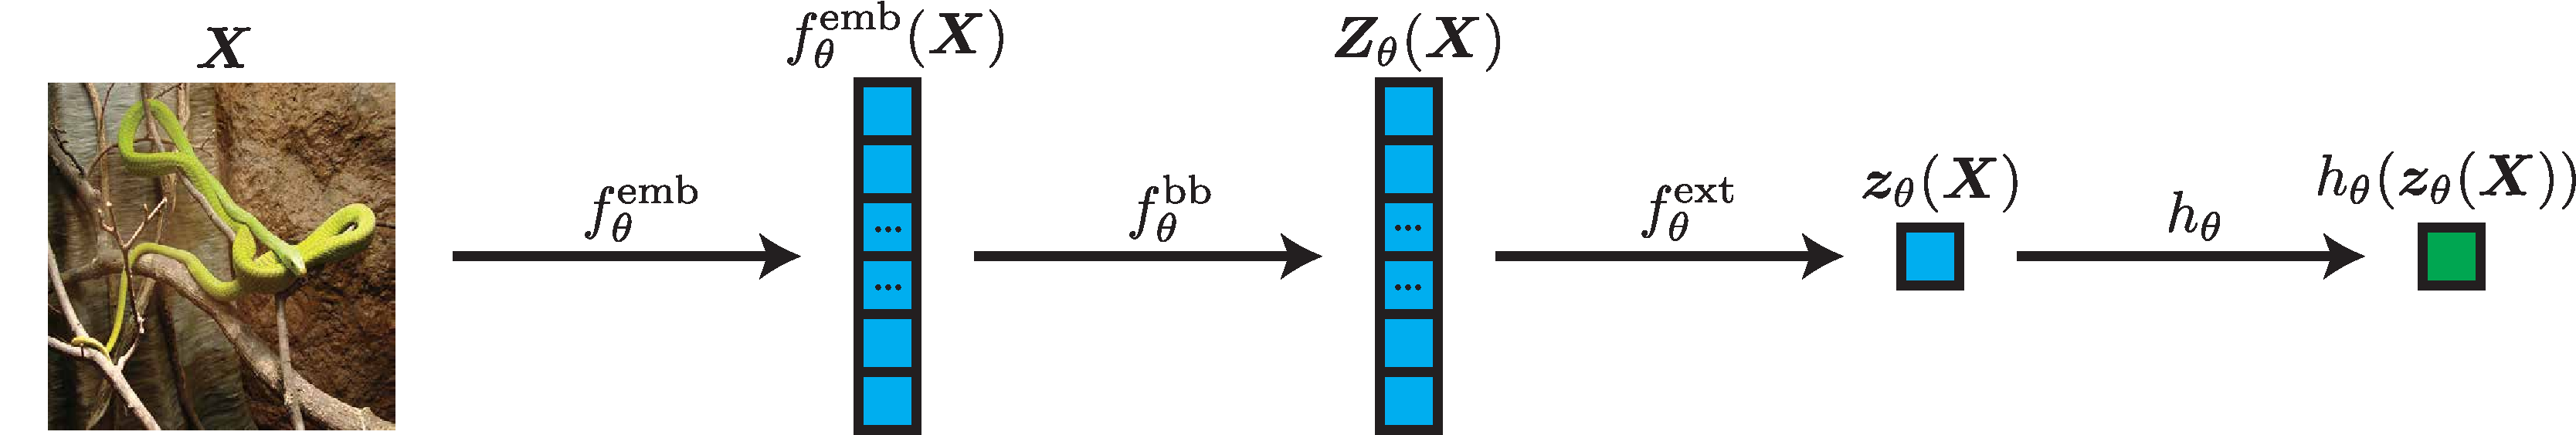
\includegraphics[width=\textwidth]{\toplevelprefix/chapters/chapter7/figs/encoder_pipeline.pdf}
    \caption{\small\textbf{编码器流程图。} 数据 \(\vX \in \cD\) 通过嵌入层 \(f_{\theta}^{\emb}\) 得到一个在 \((\R^{d})^{*}\) 空间中的序列。该嵌入序列再通过主干网络 \(f_{\theta}^{\mathrm{bb}}\) 得到每个词元的特征 \(\vZ_{\theta}(\vX)\)。我们可以使用提取映射 \(f_{\theta}^{\mathrm{ext}}\) 来得到一个聚合特征 \(\vz_{\theta}(\vX)\)。最后,为了在下游任务中使用该聚合特征,我们可以使用任务特定的头部 \(h_{\theta}\)。}
    \label{fig:overall_encoder_pipeline}
\end{figure}

\begin{figure}
    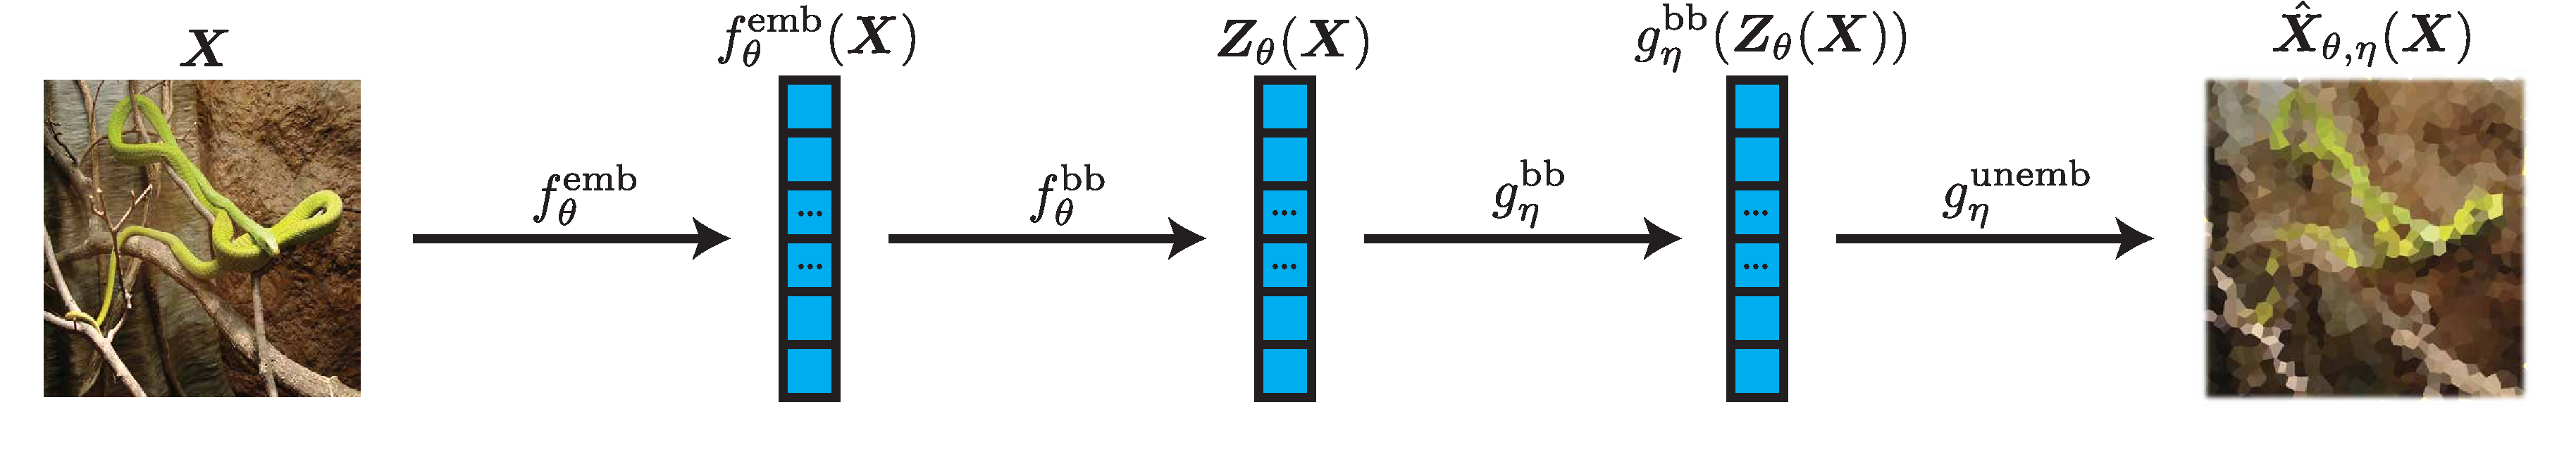
\includegraphics[width=\textwidth]{\toplevelprefix/chapters/chapter7/figs/autoencoder_pipeline.pdf}
    \caption{\small\textbf{自编码器流程图。} 数据 \(\vX \in \cD\) 通过嵌入层 \(f_{\theta}^{\emb}\) 得到一个在 \((\R^{d})^{*}\) 空间中的序列。该嵌入序列通过一个编码器主干网络 \(f_{\theta}^{\mathrm{bb}}\) 得到每个词元的特征 \(\vZ_{\theta}(\vX)\)。为了解码 \(\vZ_{\theta}(\vX)\),我们将其通过一个解码器主干网络 \(g_{\eta}^{\mathrm{bb}}\)。为了将解码器主干网络的输出映射回数据空间 \(\cD\),我们使用一个\textit{逆嵌入}层 \(g_{\eta}^{\mathrm{unemb}}\),最终得到一个重构结果 \(\hat{\vX}_{\theta, \eta}(\vX)\)(此处以输入图像的像素化重构形式进行示意)。}
    \label{fig:overall_autoencoder_pipeline}
\end{figure}

让我们将所有可能的数据集合定义为 \(\cD\)(例如,这最终将是图像集合 \(\cI\) 或文本集合 \(\cT\)),并将 \(\R^{d}\) 中词元的有限序列集合(即行数为 \(d\) 的矩阵集合)定义为 \((\R^{d})^{*} := \bigcup_{T = 1}^{\infty}\R^{d \times T}\)。为了讨论本章中介绍的众多应用,我们首先回顾一下,本书其余部分讨论了两种不同类型的模型架构。
%\yima{It would be good if we can have a diagram for each of the following two architectures, with the associated notations and terminologies...}
\begin{itemize}
    \item 一种\textit{编码器}(encoder)架构,由参数 \(\theta\) 参数化,包含以下几个组成部分:
    \begin{itemize}
        \item 一个\textit{嵌入}(embedding)层 \(f_{\theta}^{\emb} \colon \cD \to (\R^{d})^{*}\),它将输入数据 \(\cD\) 转换为一系列\textit{词元}(tokens),这些词元被映射或\textit{嵌入}到 \(D\) 维空间中。\textit{在本章的其余部分,我们常常将词元与其嵌入向量等同看待。}
        \item 一个\textit{编码器主干网络}(encoder backbone)\(f_{\theta}^{\backbone} \colon (\R^{d})^{*} \to (\R^{d})^{*}\),它使用一个序列到序列的操作来处理嵌入序列。该主干网络由前几章讨论的网络架构实现,但我们稍后会给出更正式的描述。
        \item 一个\textit{聚合特征提取器}(aggregate feature extractor)\(f_{\theta}^{\ext} \colon (\R^{d})^{*} \to \R^{d}\),它从整个序列中提取一个聚合表示。这用于为整个数据样本定义一个单一的特征。
        \item 一个\textit{任务特定头}(task-specific head)\(h_{\theta} \colon \R^{d} \to \R^{m}\),它提取一个 \(m\) 维的输出用于预测。
    \end{itemize}
    我们还定义 \(f_{\theta} := f_{\theta}^{\backbone} \circ f_{\theta}^{\emb} \colon \cD \to (\R^{d})^{*}\)。对于一个输入 \(\vX\),我们记 \(\vZ_{\theta}(\vX) := f_{\theta}(\vX)\) 和 \(\vz_{\theta}(\vX) := f_{\theta}^{\ext}(\vZ_{\theta}(\vX))\)。整个流程如 \Cref{fig:overall_encoder_pipeline} 所示。
    \item 一种\textit{自编码器}(autoencoder)架构,包含以下几个组成部分:
    \begin{itemize}
        \item 一个\textit{嵌入}层 \(f_{\theta}^{\emb} \colon \cD \to (\R^{d})^{*}\),它将输入数据 \(\cD\) 转换为一系列嵌入在 \(D\) 维空间中的\textit{词元}。
        \item 一个\textit{编码器主干网络} \(f_{\theta}^{\backbone} \colon (\R^{d})^{*} \to (\R^{d})^{*}\),它使用一个序列到序列的操作来处理嵌入序列。
        \item 一个\textit{解码器主干网络}(decoder backbone)\(g_{\eta}^{\backbone} \colon (\R^{d})^{*} \to (\R^{d})^{*}\),它在概念上是编码器主干网络操作的逆过程。
        \item 一个\textit{逆嵌入}(unembedding)层 \(g_{\eta}^{\unemb} \colon (\R^{d})^{*} \to \cD\),它作为嵌入层的逆操作。
    \end{itemize}
    我们还定义 \(f_{\theta} := f_{\theta}^{\backbone} \circ f_{\theta}^{\emb} \colon \cD \to (\R^{d})^{*}\) 和 \(g_{\eta} := g_{\eta}^{\unemb} \circ g_{\eta}^{\backbone} \colon (\R^{d})^{*} \to \cD\)。对于一个输入 \(\vX\),我们记 \(\vZ_{\theta}(\vX) := f_{\theta}(\vX)\) 和 \(\hat{\vX}_{\theta, \eta}(\vX) := g_{\eta}(\vZ_{\theta}(\vX))\)。整个流程如 \Cref{fig:overall_autoencoder_pipeline} 所示。
\end{itemize}

本章将反复使用这些符号,因此如果遇到不解之处,请随时回顾此节。我们对网络的这种分解也与大多数代码实现紧密对应,您可以从定义这些网络开始您的编码项目。

在本章中,我们将在 \Cref{sec:contrastive_learning} 中讨论本书原理在对比学习中的应用。这既是对图像数据、数据增强技术以及一种名为 Transformer 的常用架构的介绍,\textit{也}是首次展示利用本书原理可以实现何种程度的简化。接着,我们将在 \Cref{sec:image_classification,sec:clm_text} 中继续探讨对\textit{网络架构}的改进,这些改进展示了简化架构在图像和文本领域进行\textit{编码}的能力。然后,我们将在 \Cref{sec:image_completion} 中展示用于\textit{自编码}的简化架构。% We will end our discussion of principled improvements by discussing a practical implementation of the \textit{closed-loop transcription} framework in \Cref{sec:ctrl}, as well as a myriad of empirically challenging tasks which the framework drastically simplifies. 
% For the sake of completeness, we finish the chapter in \Cref{sec:training_tips} by discussing some principled tips and tricks for training models on real data.


\section{简化的对比学习}\label{sec:contrastive_learning}

学习高质量且忠实的数据表示是深度学习中的一个基本问题,被称为\textit{自监督学习}。学界已经提出了许多解决此任务的方法,其中很多并未明显使用本手稿中概述的技术和原理。其中一种方法称为\textit{对比学习}(contrastive learning),其得名原因在于其学习目标(粗略地说)是确保“相似”数据的特征相似,而“不相似”数据的特征相距甚远。对比学习的解决方案通常是高度工程化、基于经验设计的方法。在本节中,我们将描述一种名为 DINO \citep{caron2021emerging} 的方法,并运用前几章描述的原理来大幅简化其设计决策,同时提升所学表示的质量。

\subsection{数据}\label{sub:contrastive_learning_data}

我们用来探索和简化 DINO 方法论的数据均为二维图像数据。对于\textit{训练},我们将使用 ImageNet-1K 和 ImageNet-21K 数据集。数据集中的每个样本都是一张分辨率不一的 RGB 图像,并带有一个标签,指明图像所包含的物体或场景(即图像的\textit{类别})。ImageNet-1K 数据集包含 128 万张训练图像和 5 万张验证图像,共分为 1000 个类别。ImageNet-21K 数据集包含 1420 万张训练图像和 21800 个类别,但这些类别并非互不相交(即某些类别是其他类别的子集)。由于我们进行的是自监督学习,标签在训练期间不会被使用,仅在评估时使用。对于\textit{评估},我们将使用一系列数据集。其中,最常用的是 CIFAR-10。CIFAR-10 是一个包含 6 万张 32 \(\times\) 32 分辨率的 RGB 自然图像的数据集,分为 10 个类别,并预先划分为 5 万个样本的训练集和 1 万个样本的验证集。使用 CIFAR-10 的目的是为了确保在一个图像分布(ImageNet)上训练的模型能够泛化到另一个图像分布(CIFAR-10)。我们还参考了其他类似的数据集,如 CIFAR-100(与 CIFAR-10 不相交)、Oxford Flowers 和 Oxford Pets。ImageNet-1K 和 CIFAR-10 数据的示例见 \Cref{fig:in1k_cifar10_examples}。为了提高模型的鲁棒性,我们通常在处理每张图像时应用\textit{微小的数据增强},例如翻转、添加少量随机噪声或随机大面积裁剪;我们在符号表示中不包含这一点,因为自然图像的每一次增强本身(都非常接近)我们数据集中的一张自然图像。

\begin{figure}
    \centering
    
    \hfill 
    \begin{subfigure}{0.3\textwidth}
        \centering 
        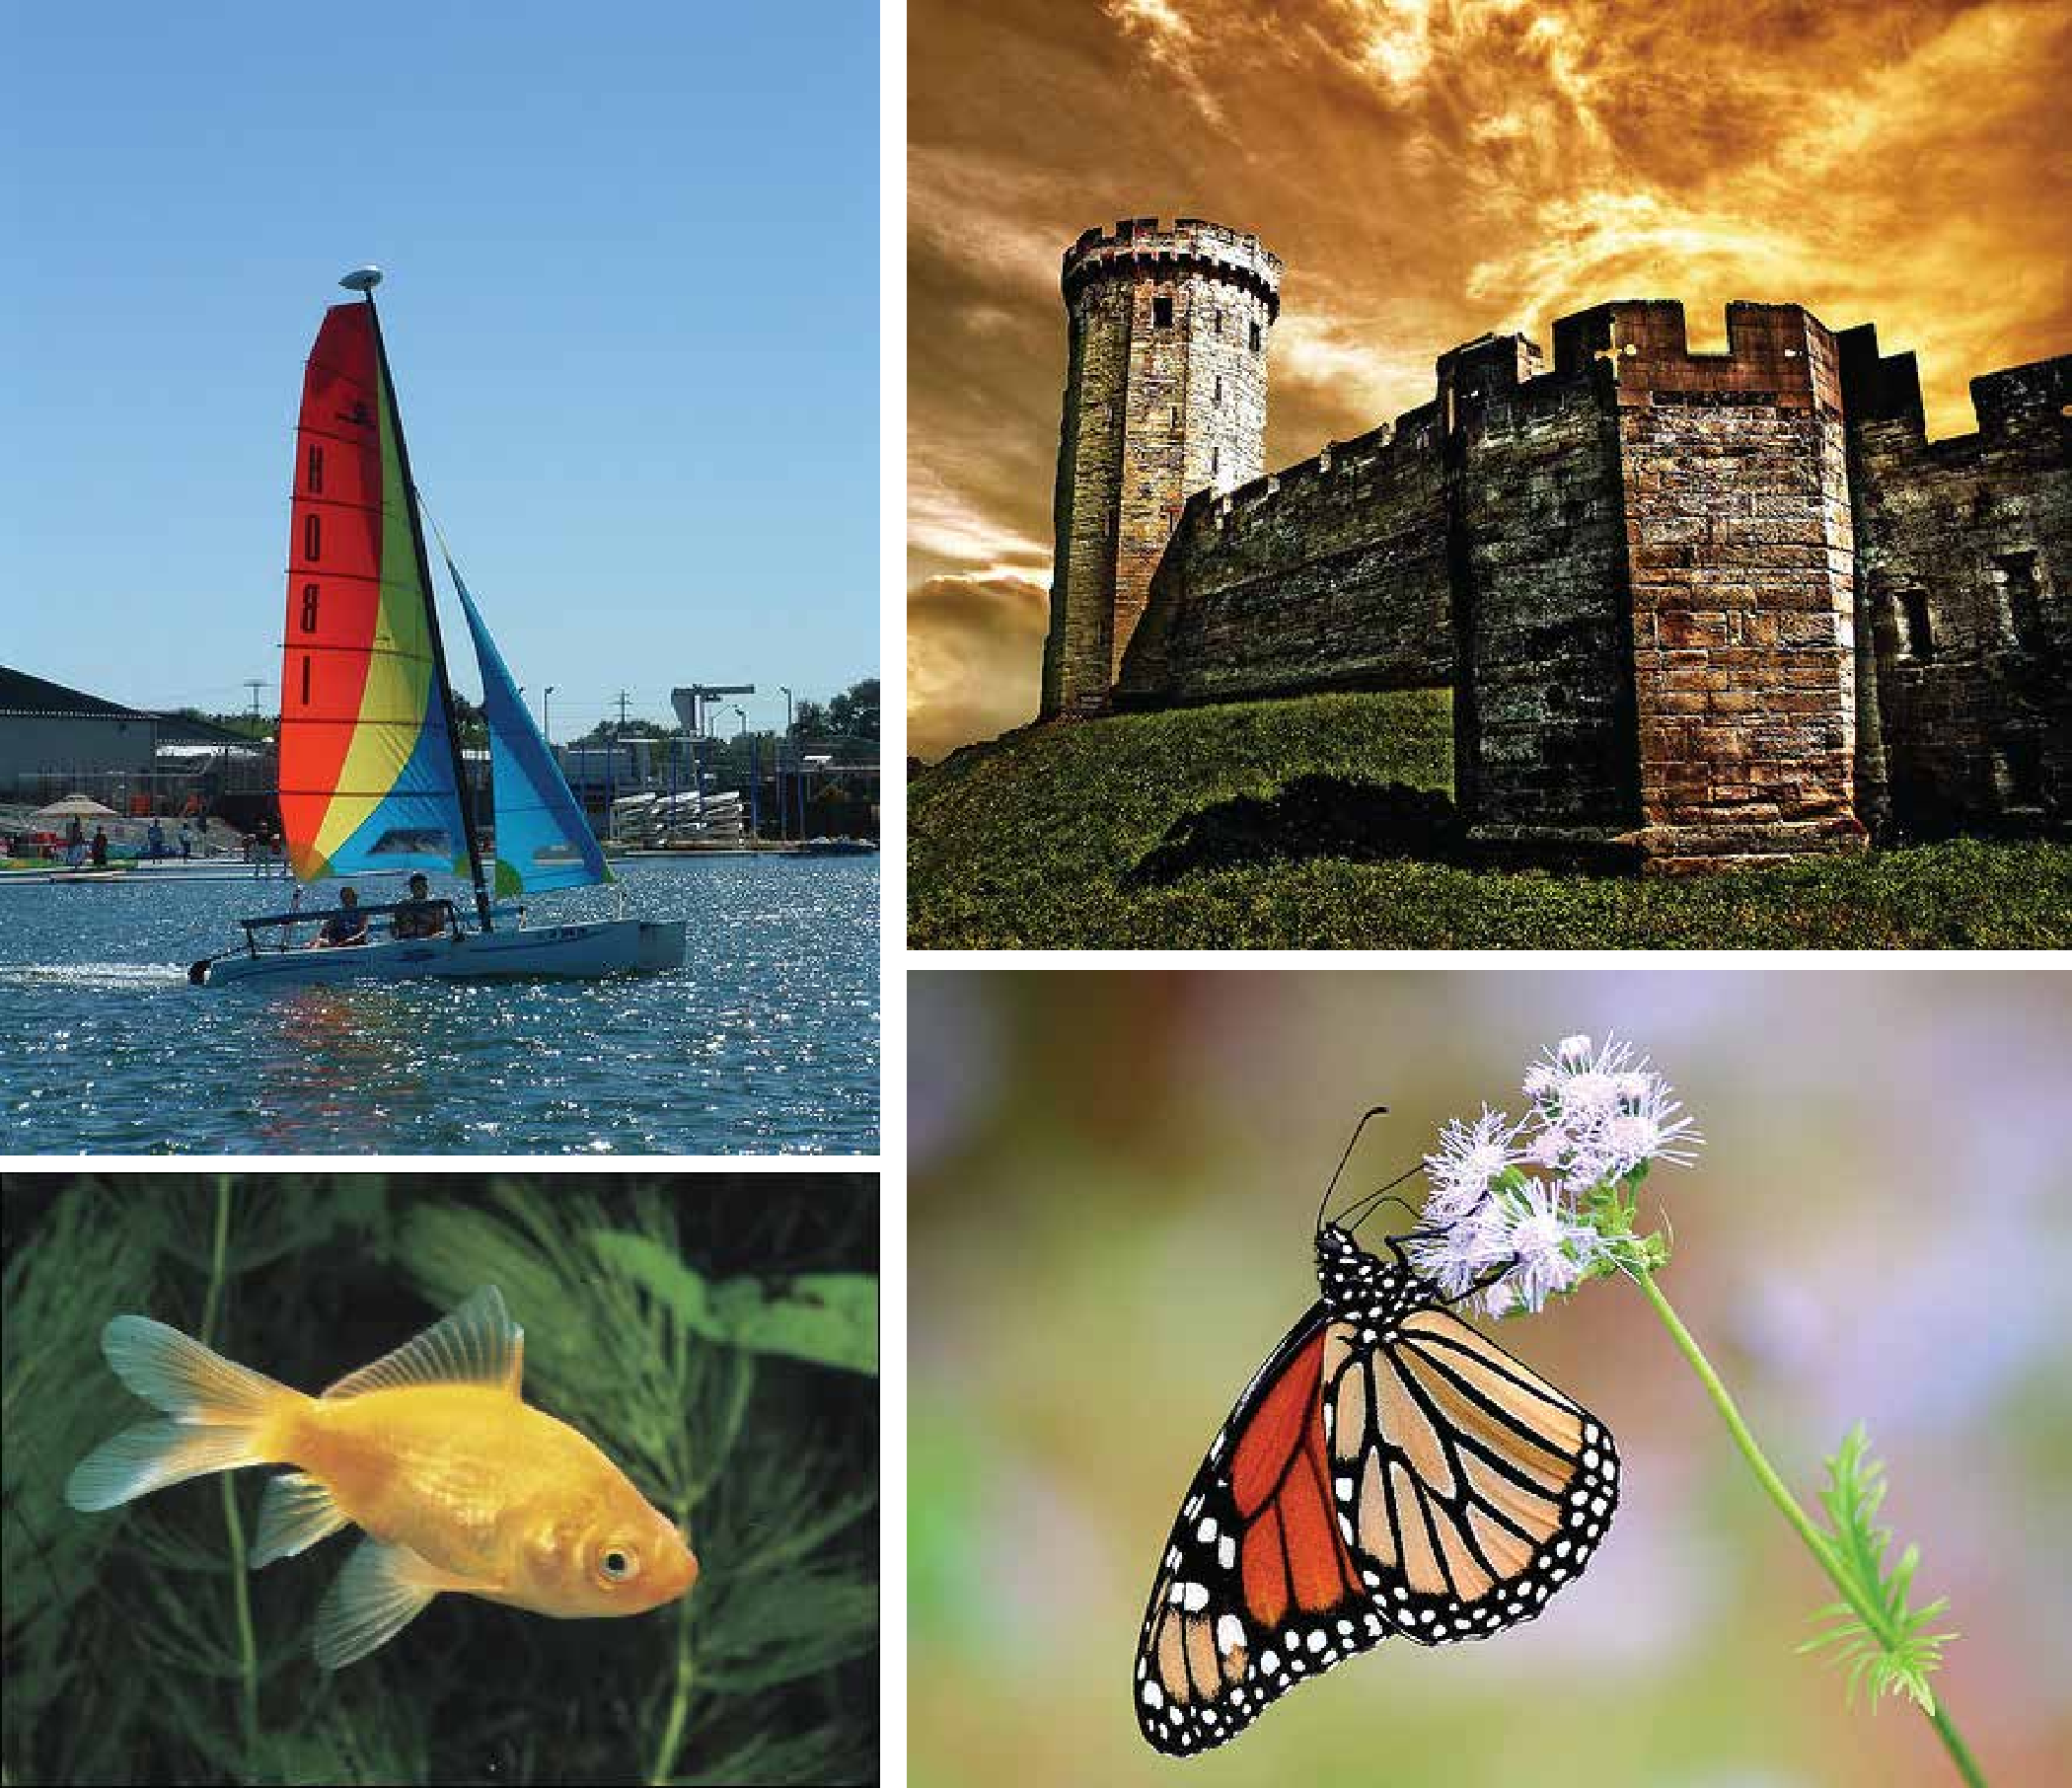
\includegraphics[width=\textwidth]{\toplevelprefix/chapters/chapter7/figs/imagenet.pdf}
        \caption{\small ImageNet-1K 样本。}
    \end{subfigure}
    \hfill 
    \begin{subfigure}{0.26\textwidth}
        \centering 
        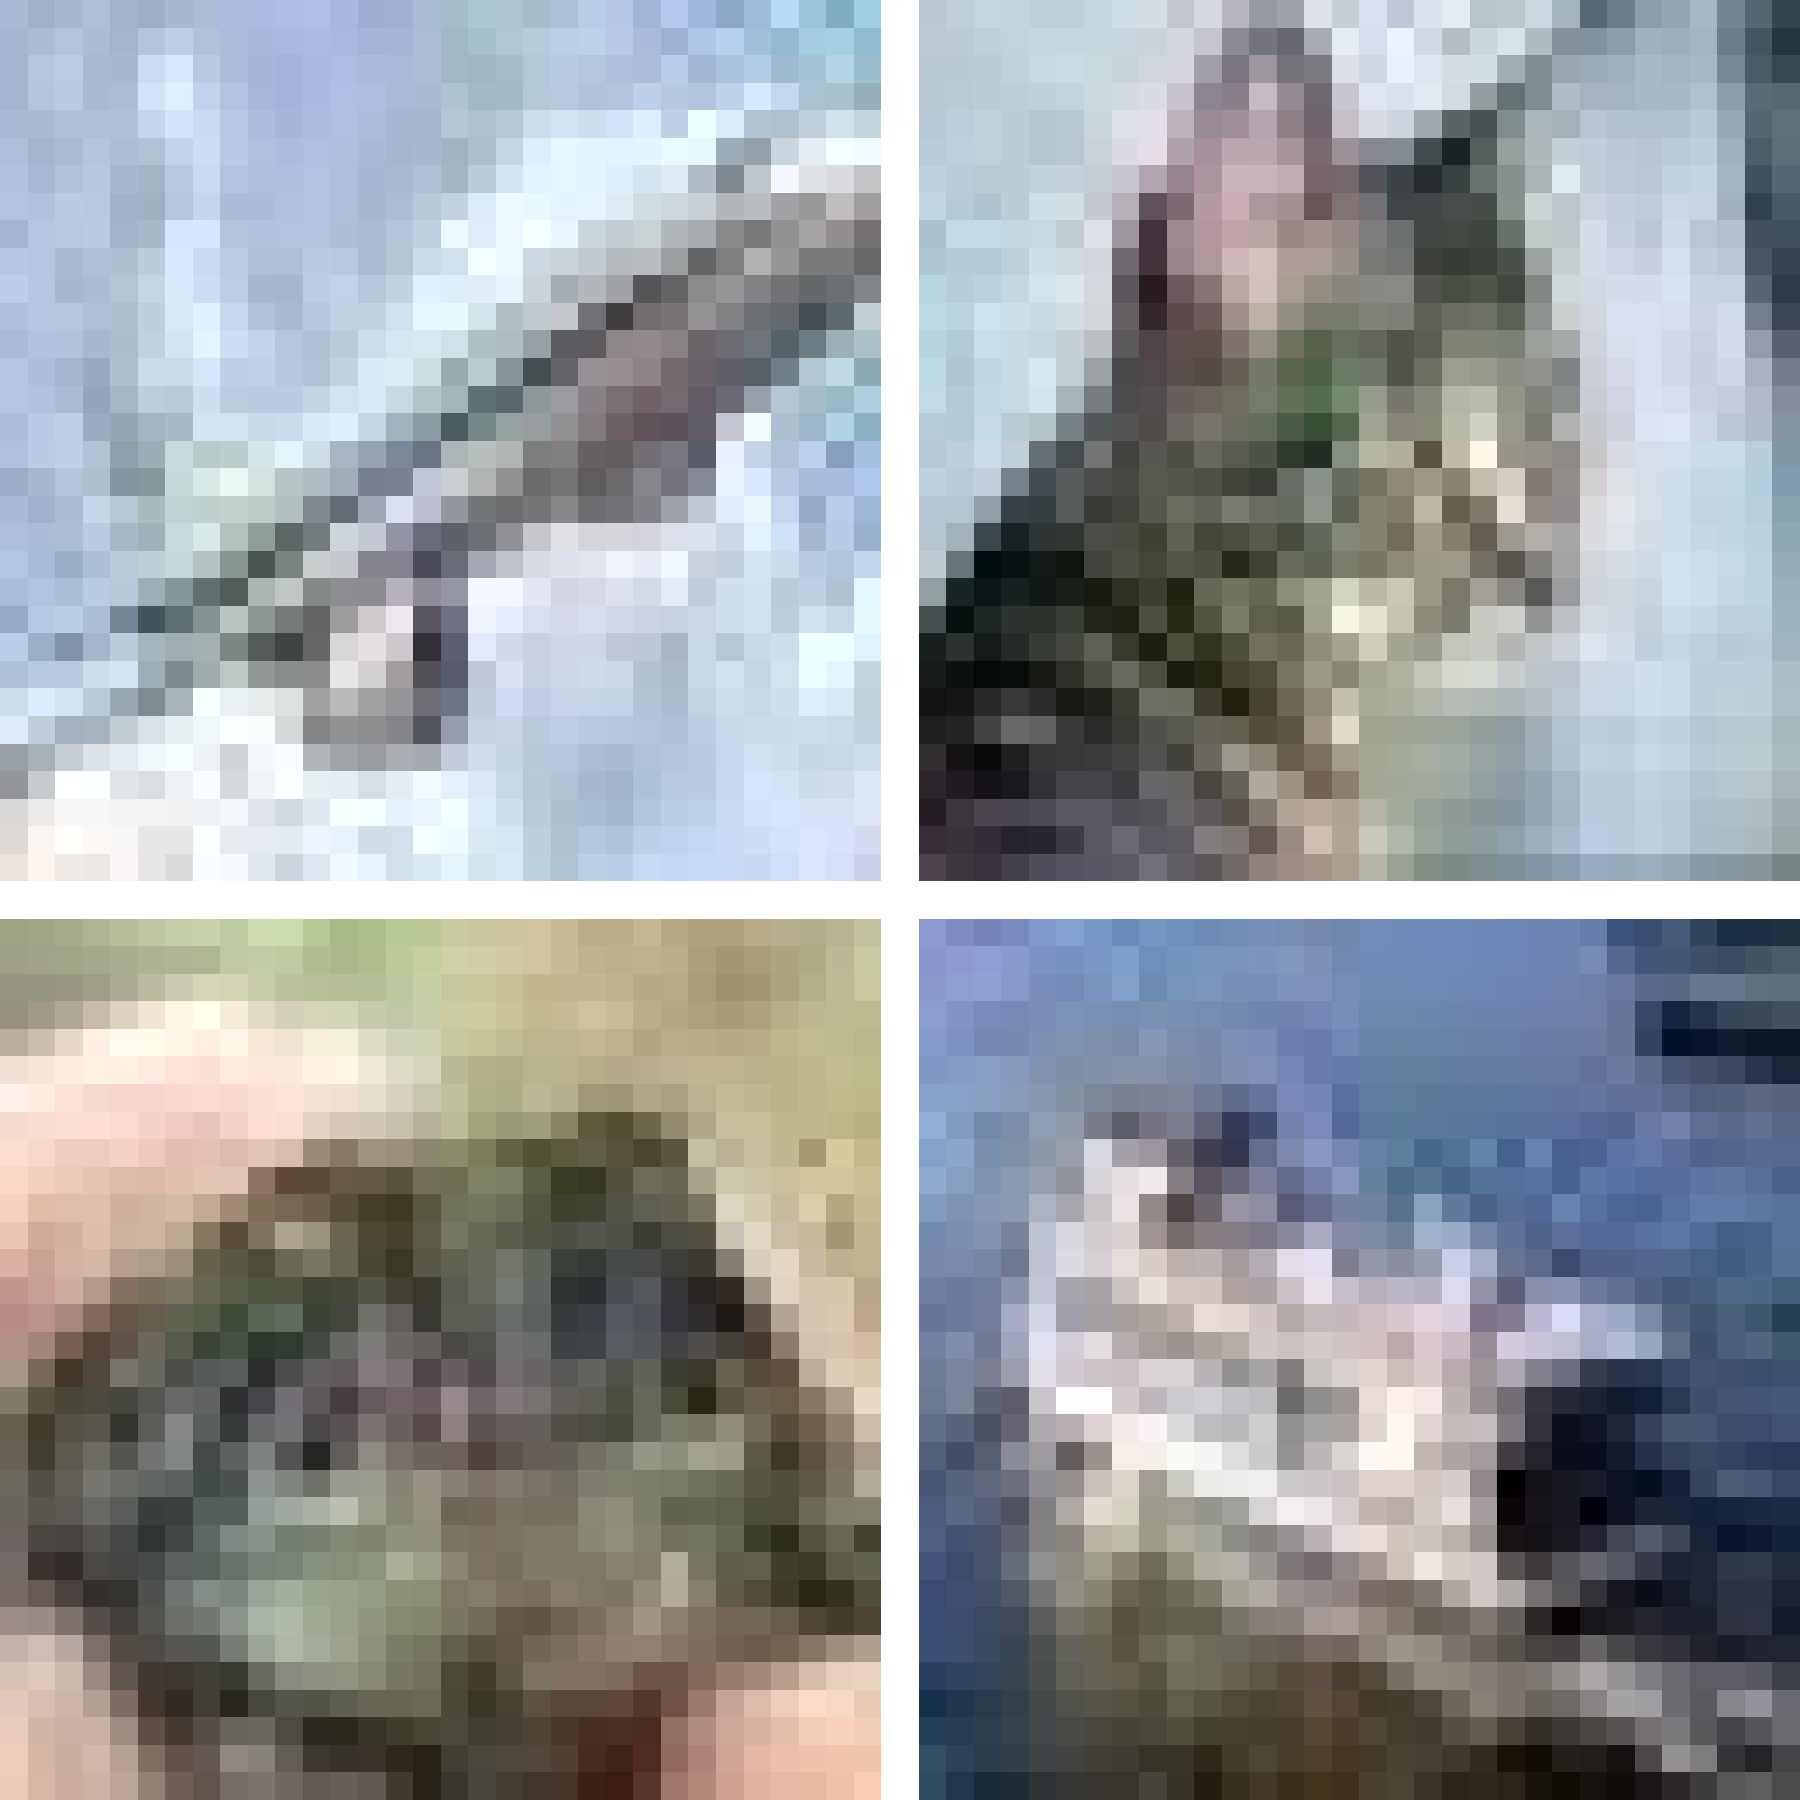
\includegraphics[width=\textwidth]{\toplevelprefix/chapters/chapter7/figs/cifar10.pdf}
        \caption{\small CIFAR-10 样本。}
    \end{subfigure}
    \hfill 
    \phantom{}

    \caption{\small\textbf{来自 ImageNet-1K(\textit{左})和 CIFAR-10(\textit{右})的图像。} 请注意,CIFAR-10 的图像分辨率通常要低得多,这降低了学习该分布的复杂性。}
    \label{fig:in1k_cifar10_examples}
\end{figure}

在更形式化的层面上,我们的数据 \(\vX\) 将是图像;我们令 \(\cI\) 为所有图像的集合。由于图像是像素的矩形阵列,每个像素的颜色由 RGB、CMYK 或其他颜色格式给出,我们称一张图像是 \(\R^{c \times h \times w}\) 中的一个元素——这里 \(c\) 是通道数(例如,RGB 为 \(3\),CMYK 为 \(4\)),\(h\) 是图像高度,\(w\) 是图像宽度。因此,所有图像的集合 \(\cI := \bigcup_{c, h, w = 1}^{\infty}\R^{c \times h \times w}\) 是所有此类可能数据的集合。同样,我们将反复使用这个符号。


\subsection{任务与目标函数} \label{sub:contrastive_learning_objective}

我们的任务是学习数据的一个良好表示。对比学习大体上是通过定义我们希望特征反映输入图像的哪些属性,构造共享这些属性但其他属性不同的图像,并设立一个损失函数来促使共享属性的图像特征相近,而不同属性的图像特征相异。这个学习问题的自然最优解是,所学的特征保留了输入的期望属性。然而,在训练对比学习模型的过程中,会出现许多实际和经验上的复杂问题。

在 DINO 的案例中,作者提出使用一种方法,为整个图像生成一个单一的特征向量,并期望该特征向量包含“全局”(即图像级别)信息。相应地,损失函数将促使具有相似全局信息的图像拥有相似的特征,而具有不同全局信息的图像拥有不同的特征。

这听起来很直观,但如前所述,即使在设置损失函数时也存在一些经验上的考量。首先,我们应该如何促进相似性和差异性?DINO \citep{caron2021emerging} 的答案是\footnote{在笔者看来,这有些令人费解……}将输出特征转换为对应于某个概率分布的“logits”,并计算它们的交叉熵。更具体地说,令 \(\Delta_{m} := \{\vx \in \R^{m} \colon x_{i} \geq 0\ \forall i \in [m], \sum_{i = 1}^{m}x_{i} = 1\}\) 为 \(\R^{m}\) 中的概率向量空间,并定义函数 \(d_{\CE} \colon \R^{m} \times \R^{m} \to \R\) 如下:
 \begin{equation}\label{eq:cross_entropy_difference}
    d_{\CE}(\vp, \vq) := \CE(\vp, \vq), \quad \forall \vp, \vq \in \Delta_{m}
 \end{equation}
 其中 \(\CE \colon \Delta_{m} \times \Delta_{m} \to \R\) 是交叉熵,定义为
 \begin{equation}\label{eq:expts_def_ce}
    \CE(\vp, \vq) := -\sum_{i = 1}^{m}p_{i}\log q_{i}, \quad \forall \vp = (p_{1}, \dots, p_{m}), \vq = (q_{1}, \dots, q_{m}) \in \Delta_{m}.
 \end{equation}
 在我们继续讨论之前,让我们先建立一些关于这个距离函数的直观理解。我们有,特别地,
 \begin{align}
    \CE(\vp, \vq)
    &= -\sum_{i = 1}^{m}p_{i}\log q_{i} = \sum_{i = 1}^{m}p_{i}\log(p_{i}/q_{i}) - \sum_{i = 1}^{m}p_{i}\log p_{i} = \KL(\vp, \vq) + H(\vp)
 \end{align}
 其中 \(\KL \colon \Delta_{m} \times \Delta_{m} \to \R\) 是 KL 散度,定义为
 \begin{equation}
    \KL(\vp, \vq) := \sum_{i = 1}^{m}p_{i}\log(p_{i}/q_{i}),
 \end{equation}
 而 \(H \colon \Delta_{m} \to \R\) 是一个随机变量的熵。注意 \(\KL(\vp, \vq)\) 当且仅当 \(\vp = \vq\) 时最小化。所以最小化 \(d_{\CE}\) 有两个作用:它使得 \(\vp = \vq\),并且它使得 \(\vp\) 和 \(\vq\) 的熵最小(即,在一个分量上为 \(1\),其他分量为 \(0\) 的向量——这些被称为\textit{独热向量}(one-hot vectors))。总的来说,这个目标不仅是为了匹配 \(\vp\) 和 \(\vq\),而且还以某种方式塑造它们,使它们成为低熵向量。在讨论公式时请记住这一点。

接下来的问题是,我们应该如何获得具有相似全局信息的样本?DINO(以及几乎所有的对比学习)的答案是\textit{数据增强}(data augmentation)——从每个样本中,生成几个相关的、共享期望属性的样本。在 DINO 的案例中,我们使用输入图像的不同裁剪或\textit{视图}(views)。回想一下,我们将图像建模为集合 \(\cI\) 的一个元素。在这个记法中,一个视图是一个函数 \(v \colon \cI \to \cI\)。在 DINO 的案例中,视图是\textit{随机缩放裁剪}(random resized crop):它从图像中随机选取一个矩形裁剪区域(其面积占图像总面积的固定百分比 \(p_{v} \in [0, 1]\)),按比例调整其大小,使得\textit{较短的边}长为 \(S_{\rsz}\) 像素,然后将其调整为固定的形状 \((C, S_{v}, S_{v})\),其中 \(S_{v} \geq 1\) 是视图的大小,\(C\) 是原始图像的通道数。

\begin{figure}
    \centering 
    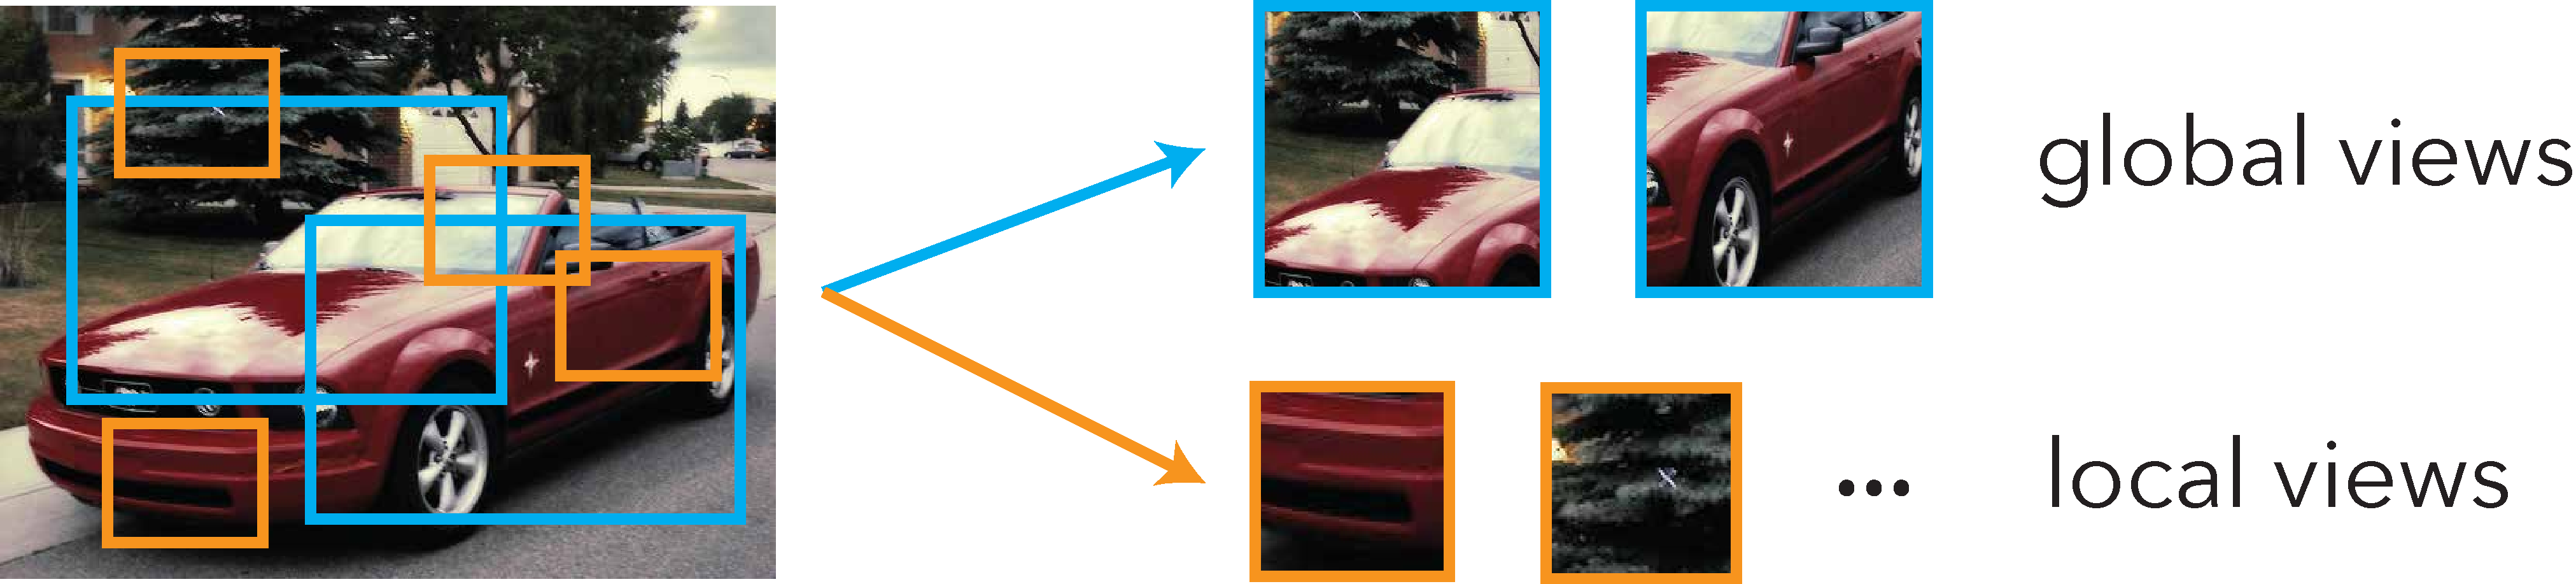
\includegraphics[width=0.7\textwidth]{\toplevelprefix/chapters/chapter7/figs/global_local_views.pdf}
    \caption{\textbf{DINO 中的局部视图和全局视图。} 局部视图和全局视图从输入图像中取一个矩形裁剪区域,并将其调整为正方形,然后输入网络进行处理。}
    \label{fig:dino_local_global_views}
\end{figure}

我们希望使用两种类型的视图,如 \Cref{fig:dino_local_global_views} 所示:
\begin{itemize}
    \item \textit{全局视图}(global views),是面积百分比参数为 \(p_{\glo} \in [0, 1]\) 且输出形状为 \((C, S_{\glo}, S_{\glo})\) 的随机缩放裁剪;
    \item 以及\textit{局部视图}(local views),是面积百分比参数为 \(p_{\loc} \in [0, 1]\) 且输出形状为 \((C, S_{\loc}, S_{\loc})\) 的随机缩放裁剪。这里 \(p_{\loc} < p_{\glo}\) 且 \(S_{\loc} < S_{\glo}\)。
\end{itemize}

DINO 期望输入图像 \(\vX\) 的所有视图 \(\vX_{v} := v(\vX)\) 的聚合特征 \(\vz_{\theta}(\vX_{v}) := (f_{\theta}^{\ext} \circ f_{\theta})(\vX_{v})\) 彼此一致。DINO 通过使用一个\textit{“DINO 头”}\footnote{注意,\(h_{\vW, \vmu}\) 是任务特定头,在 \Cref{sec:experiment_setup} 中仅由 \(\theta\) 参数化,而不是任何特定参数。但由于我们用第二个参数的不同值两次调用 \(h\),我们保留了指定的符号。} \(h_{\vW, \vmu}\),由一个矩阵 \(\vW \in \R^{s \times d}\) 和一个向量 \(\vmu \in \R^{s}\) 参数化,从聚合特征 \(\vz_{\theta}(\vX_{v})\) 中提取一个概率向量 \(\vp_{\theta, \vW, \vmu}(\vX_{v}) := h_{\vW, \vmu}(\vz_{\theta}(\vX_{v}))\),使用以下简单的配方:
\begin{equation}
    h_{\vW, \vmu}(\vz) := \softmax([\vW\vz - \vmu]/\tau), \qquad \forall \vz \in \R^{d},
\end{equation}
其中 \(\softmax \colon \R^{s} \to \Delta_{s}\) 函数定义为
\begin{equation}
    \softmax\rp{\mat{x_{1} \\ \vdots \\ x_{s}}} := \frac{1}{\sum_{i = 1}^{s}e^{x_{i}}}\mat{e^{x_{1}} \\ \vdots \\ e^{x_{s}}}
\end{equation}
而 \(\tau > 0\) 是一个“温度”参数,控制 softmax 输出的熵。

特别地,DINO 最小化每个全局视图 \(\vX_{g} := v_{g}(\vX)\) 的概率向量 \(\vp_{\theta, \vW, \vmu}(\vX_{g}) := h_{\vW, \vmu}(\vz_{\theta}(\vX_{g}))\) 与每个视图 \(\vX_{c} := v_{c}(\vX)\) 的概率向量 \(\vp_{\theta, \vW}(\vX_{c}) := h_{\vW, \vzero_{m}}(\vz_{\theta}(\vX_{c}))\) 之间的差异。这里,\(v_{c}\) 可以是局部视图\textit{或}全局视图。我们将在 \Cref{sub:contrastive_learning_architecture} 中很快讨论 \(f_{\theta}\) 和 \(f_{\theta}^{\ext}\) 的实现。总的来说,DINO 解决的问题是
 \begin{equation}\label{eq:dino_loss}
     \min_{\theta, \vW, \vmu}\cL_{\dino}(\theta, \vW, \vmu) \qquad \text{其中} \qquad \cL_{\dino}(\theta, \vW, \vmu) := \Ex[d_{\CE}(\vp_{\theta, \vW, \vmu}(\vX_{g}), \vp_{\theta, \vW}(\vX_{c}))],
\end{equation}
其中期望是对数据 \(\vX\)、全局视图 \(v_{g}\) 和其他视图 \(v_{c}\) 取的。

然而,在这种特定情况下,如果你试图实现 \eqref{eq:dino_loss} 并在真实网络上进行优化,你很可能会遇到一个问题:在运行几轮学习算法后,特征映射 \(f_{\theta}^{\ext} \circ f_{\theta}\) 将\textit{变成一个常数函数}!这当然能优化上述损失,因为它最小化了同一图像不同视图特征之间的距离。但我们显然不希望学到这种解。

实际上,避免坍塌(collapse)是对比学习中一个非常普遍的考量。那么在这种情况下该如何做呢?DINO 的解决方案同样是经验设计的,它仔细调整了参数 \(\vmu\) 的优化(该参数使用批次中的所有样本进行更新)和一个“温度”超参数 \(\tau\)(它是 \(h_{\vW, \vmu}\) 实现的一部分,并在 \Cref{sub:contrastive_learning_architecture} 中讨论)。给定一组效果良好的特殊超参数,这确实足以确保表示不会坍塌。然而,在这种特殊配置之外,训练模型使其收敛是困难的,且训练过程高度不稳定。

为了改善这种状况,让我们来讨论对公式的简化。首先,我们可以\textit{直接使用聚合表示},而不是使用一个学习到的变换 \(h_{\vW, \vmu}\) 来计算聚合特征 \(\vz_{\theta}\) 的概率向量,即忽略任务特定头(或等价地,将其设置为恒等映射)。但现在我们需要一种直接比较这些向量的方法。根据我们在 \Cref{ch:representation} 中提出的假设,即好的表示应该具有欧几里得(子空间)几何结构,一个更自然的差异度量是\textit{平方 \(\ell^{2}\) 距离} \(d_{\ell^{2}} \colon \R^{d} \times \R^{d} \to \R\),定义为
\begin{equation}\label{eq:cosine_similarity}
    d_{\ell^{2}}(\vx, \vy) := \frac{1}{2}\norm{\vx - \vy}_{2}^{2}, \qquad  \forall \vx, \vy \in \R^{d}.
\end{equation}
这种基于距离的评分甚至比交叉熵评分计算起来更高效。因此,在我们的简化方案中,\(d_{\ell^{2}}\) 取代了 \(d_{\CE}\)。

之前,坍塌是通过更新 \(\vmu\) 和 \(\tau\) 的技巧来避免的。在我们的简化方案中,如果我们在表示空间内比较特征而不是将它们转换为概率,我们就没有这两个参数,因此必须考虑一种不同的方式来避免坍塌。为此,我们回到基本原理。避免坍塌的基本思想是,为了确保所有样本不会返回完全相同的特征,我们需要不同样本具有不同的特征。换句话说,我们希望特征的\textit{协方差}在某种意义上是\textit{大的}。但是从 \Cref{ch:compression,ch:representation} 中,我们已经有了一个衡量协方差矩阵大小的量。也就是说,我们使用直截了当的(总体层面上的)\textit{高斯编码率}(Gaussian coding rate)\(R\) 来确保不同图像的全局视图(它们具有不同的全局信息)的特征是良好分离且不坍塌的(因此是扩展的)。修改后的总损失 \(\cL_{\simdino}\) 变为:
\begin{equation}\label{eq:simdino_loss}
    \cL_{\simdino}(\theta) := \Ex[d_{\ell^{2}}(\vz_{\theta}(\vX_{g}), \vz_{\theta}(\vX_{c}))] - \frac{\gamma}{2}\logdet\rp{\vI + \frac{d}{\eps^{2}}\Cov(\vz_{\theta}(\vX_{g}))},
\end{equation}
其中 \(\eps > 0\) 是固定的,并且适当的期望如前所述,是对数据 \(\vX\)、全局视图 \(v_{g}\) 和其他(局部或全局)视图 \(v_{c}\) 取的。公式 \eqref{eq:simdino_loss} 中的损失是用于简化 DINO(“SimDINO”)的损失。正如我们将看到的,当正确实现时,它的效果至少和原始 DINO 一样好。

\subsection{架构:视觉 Transformer}\label{sub:contrastive_learning_architecture}

对于架构,我们使用一个标准的视觉 Transformer(Vision Transformer)。下面将正式介绍这种架构在图像数据背景下的工作原理。回顾 \Cref{sec:experiment_setup},一个编码器架构有四个组成部分,即嵌入层、主干网络、特征提取器和任务特定头。我们现在讨论这三个部分。

\begin{figure}
    \centering 
    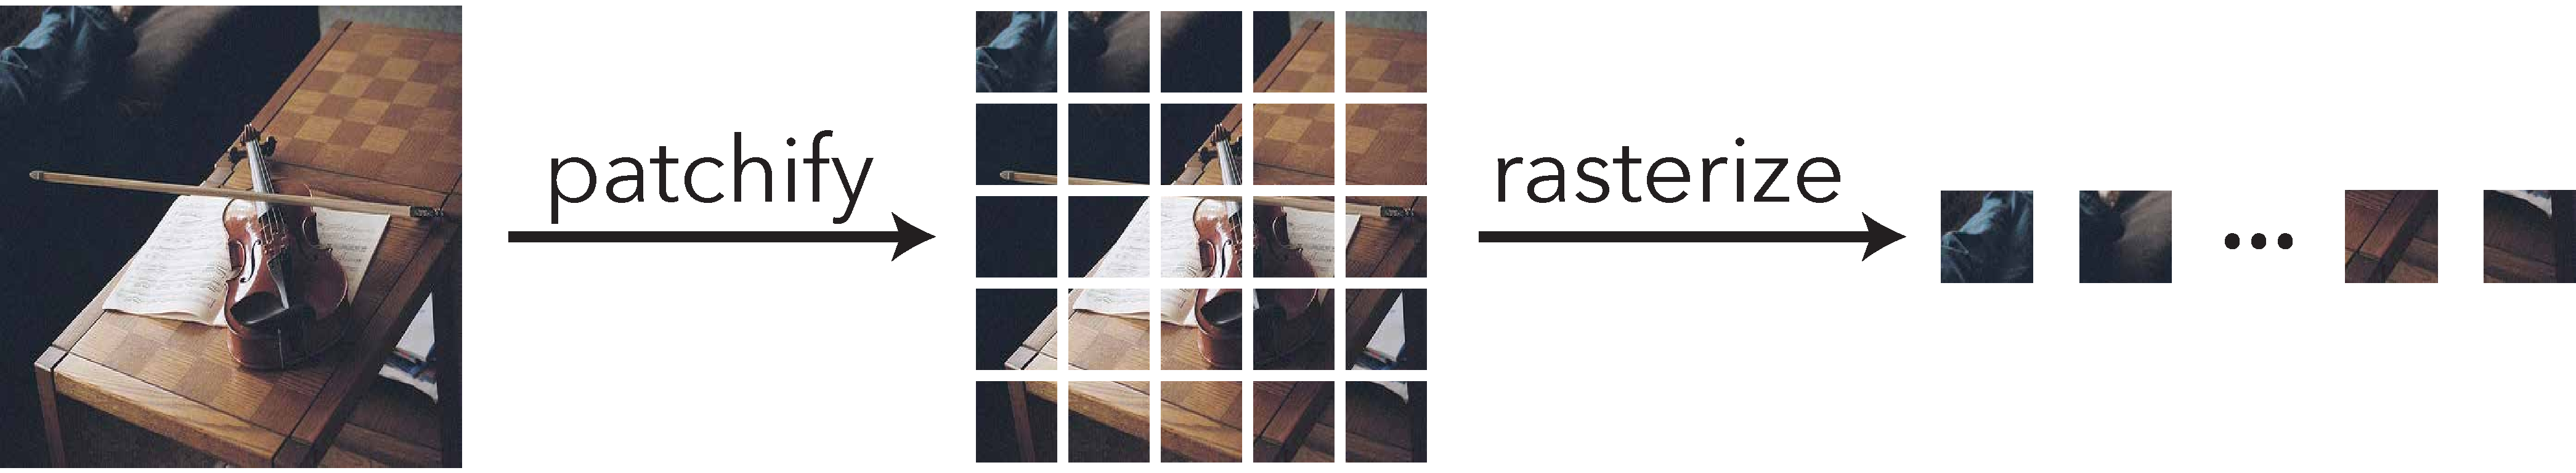
\includegraphics[width=0.8\textwidth]{\toplevelprefix/chapters/chapter7/figs/patchify.pdf}
    \caption{\small\textbf{一个将图像转换为 \(5 \times 5\) 个正方形图像块,并按光栅顺序排列的示例。} 每个图像块大小相同,图像块网格的形状为 \((N_{H}, N_{W}) = (5, 5)\)。然后,图像块网格按光栅顺序展开成一个长度为 \(5 \times 5 = 25\) 的序列。}
    \label{fig:patchify_rasterize}
\end{figure}

\begin{figure}
    \centering 
    
\includegraphics[width=\textwidth]{\toplevelprefix/chapters/chapter7/figs/transformer_embedding.pdf}
    \caption{\small\textbf{Transformer 嵌入流程。} 给定一个按光栅顺序展开的图像块序列 \(\vX^{\patch}\),每个展开的图像块被线性投影到特征空间,并配备一个(加性的)位置编码和一个称为类别词元的额外词元。输出是第一层的输入特征 \(\vZ_{\theta}^{1}(\vX) = f_{\theta}^{\emb}(\vX)\)。}
    \label{fig:transformer_embedding}
\end{figure}

\paragraph{嵌入(Embedding)。} 给定图像数据 \(\vX \in \cI\),我们使用映射 \(f_{\theta}^{\emb}\) 将其嵌入为 \(\R^{d}\) 中的一个词元序列,过程如下。前两个步骤如 \Cref{fig:patchify_rasterize} 所示,后两个步骤如 \Cref{fig:transformer_embedding} 所示。
\begin{enumerate}
    \item 首先,我们将图像数据 \(\vX\) 转换成一个形状为 \((C, P_{H}, P_{W})\) 的图像块(patch)序列,其中 \(P_{H}\) 和 \(P_{W}\) 是图像块的维度。我们假设 \(P_{H}\) 和 \(P_{W}\) 分别能整除 \(\vX\) 的高度和宽度(在 \Cref{sub:contrastive_learning_objective} 的记法中,我们假设 \(P_{H}\) 和 \(P_{W}\) 能整除 \(S_{\loc}\) 和 \(S_{\glo}\))。设得到的图像块网格有 \(N_{H}\) 行和 \(N_{W}\) 列。
    \item 我们将每个图像块展开成一个长度为 \(D := CP_{H}P_{W}\) 的向量。共有 \(N := N_{H}N_{W}\) 个图像块向量,我们将它们按“光栅顺序”(从左上到右上,再到左下到右下)排列成一个矩阵 \(\vX^{\patch} \in \R^{D \times N}\),其中 \(\vX^{\patch} := f^{\patch}(\vX)\)。注意,\(D\) 只取决于图像块大小和通道数。由于后者在同一数据集的样本中通常是恒定的,所以 \(D\) 对数据集中所有图像都相同,而 \(N\) 对于较大和较小的图像则不同。
    \item 然后我们对 \(\vX^{\patch} \in \R^{D \times N}\) 进行以下操作,将其投影到 \(\R^{d \times n}\),其中 \(n := N + 1\):
    \begin{equation}
        \vX^{\patch} \mapsto [\vz_{\cls}^{1}, \vW^{\emb}\vX] + \vE^{\pos}.
    \end{equation}
    这里我们有三个可训练的参数 \(\vW^{\emb}\)、\(\vz_{\cls}^{1}\) 和 \(\vE^{\pos}\),其作用如下:
    \begin{itemize}
        \item \(\vW^{\emb} \in \R^{d \times D}\) 是一个矩阵,它将每个图像块向量投影为一个词元特征。
        \item \(\vz_{\cls}^{1} \in \R^{d}\) 是一个所谓的\textit{类别词元}(class token)或\textit{注册词元}(register token)。类别词元启发式地持有整个数据的全局信息,并用于下游任务。在 \Cref{ch:representation} 的压缩深度网络框架中,我们期望在正向传播过程中,类别词元与显著或语义相关的词元被投影到相同的子空间上。
        \item \(\vE^{\pos} \in \R^{d \times N}\) 是一个所谓的\textit{位置编码}(positional encoding),用于区分不同图像块的词元。也就是说,词元特征应该包含位置信息,这样整体映射 \(f^{\pre}\) 就不会对图像块的排列保持不变,而 \(\vE^{\pos}\) 插入了这种位置信息。
        \begin{itemize}
            \item 在 DINO 这个案例中,Transformer 接收不同大小的图像,我们为训练期间接收到的最大尺寸学习一个位置编码,并通过插值得到较小尺寸输入的位置编码。
        \end{itemize}
    \end{itemize}
\end{enumerate}
因此,最终我们有
\begin{equation}\label{eq:definition_of_embedding_module}
    f_{\theta}^{\emb}(\vX) := \mat{\vz_{\cls}^{1}, \vW^{\emb}f^{\patch}(\vX) + \vE^{\pos}}.
\end{equation}
所有参数 \(\vz_{\cls}^{1}, \vW^{\emb}, \vE^{\pos}\) 都包含在参数集 \(\theta\) 中。

\begin{figure}
    \centering 
    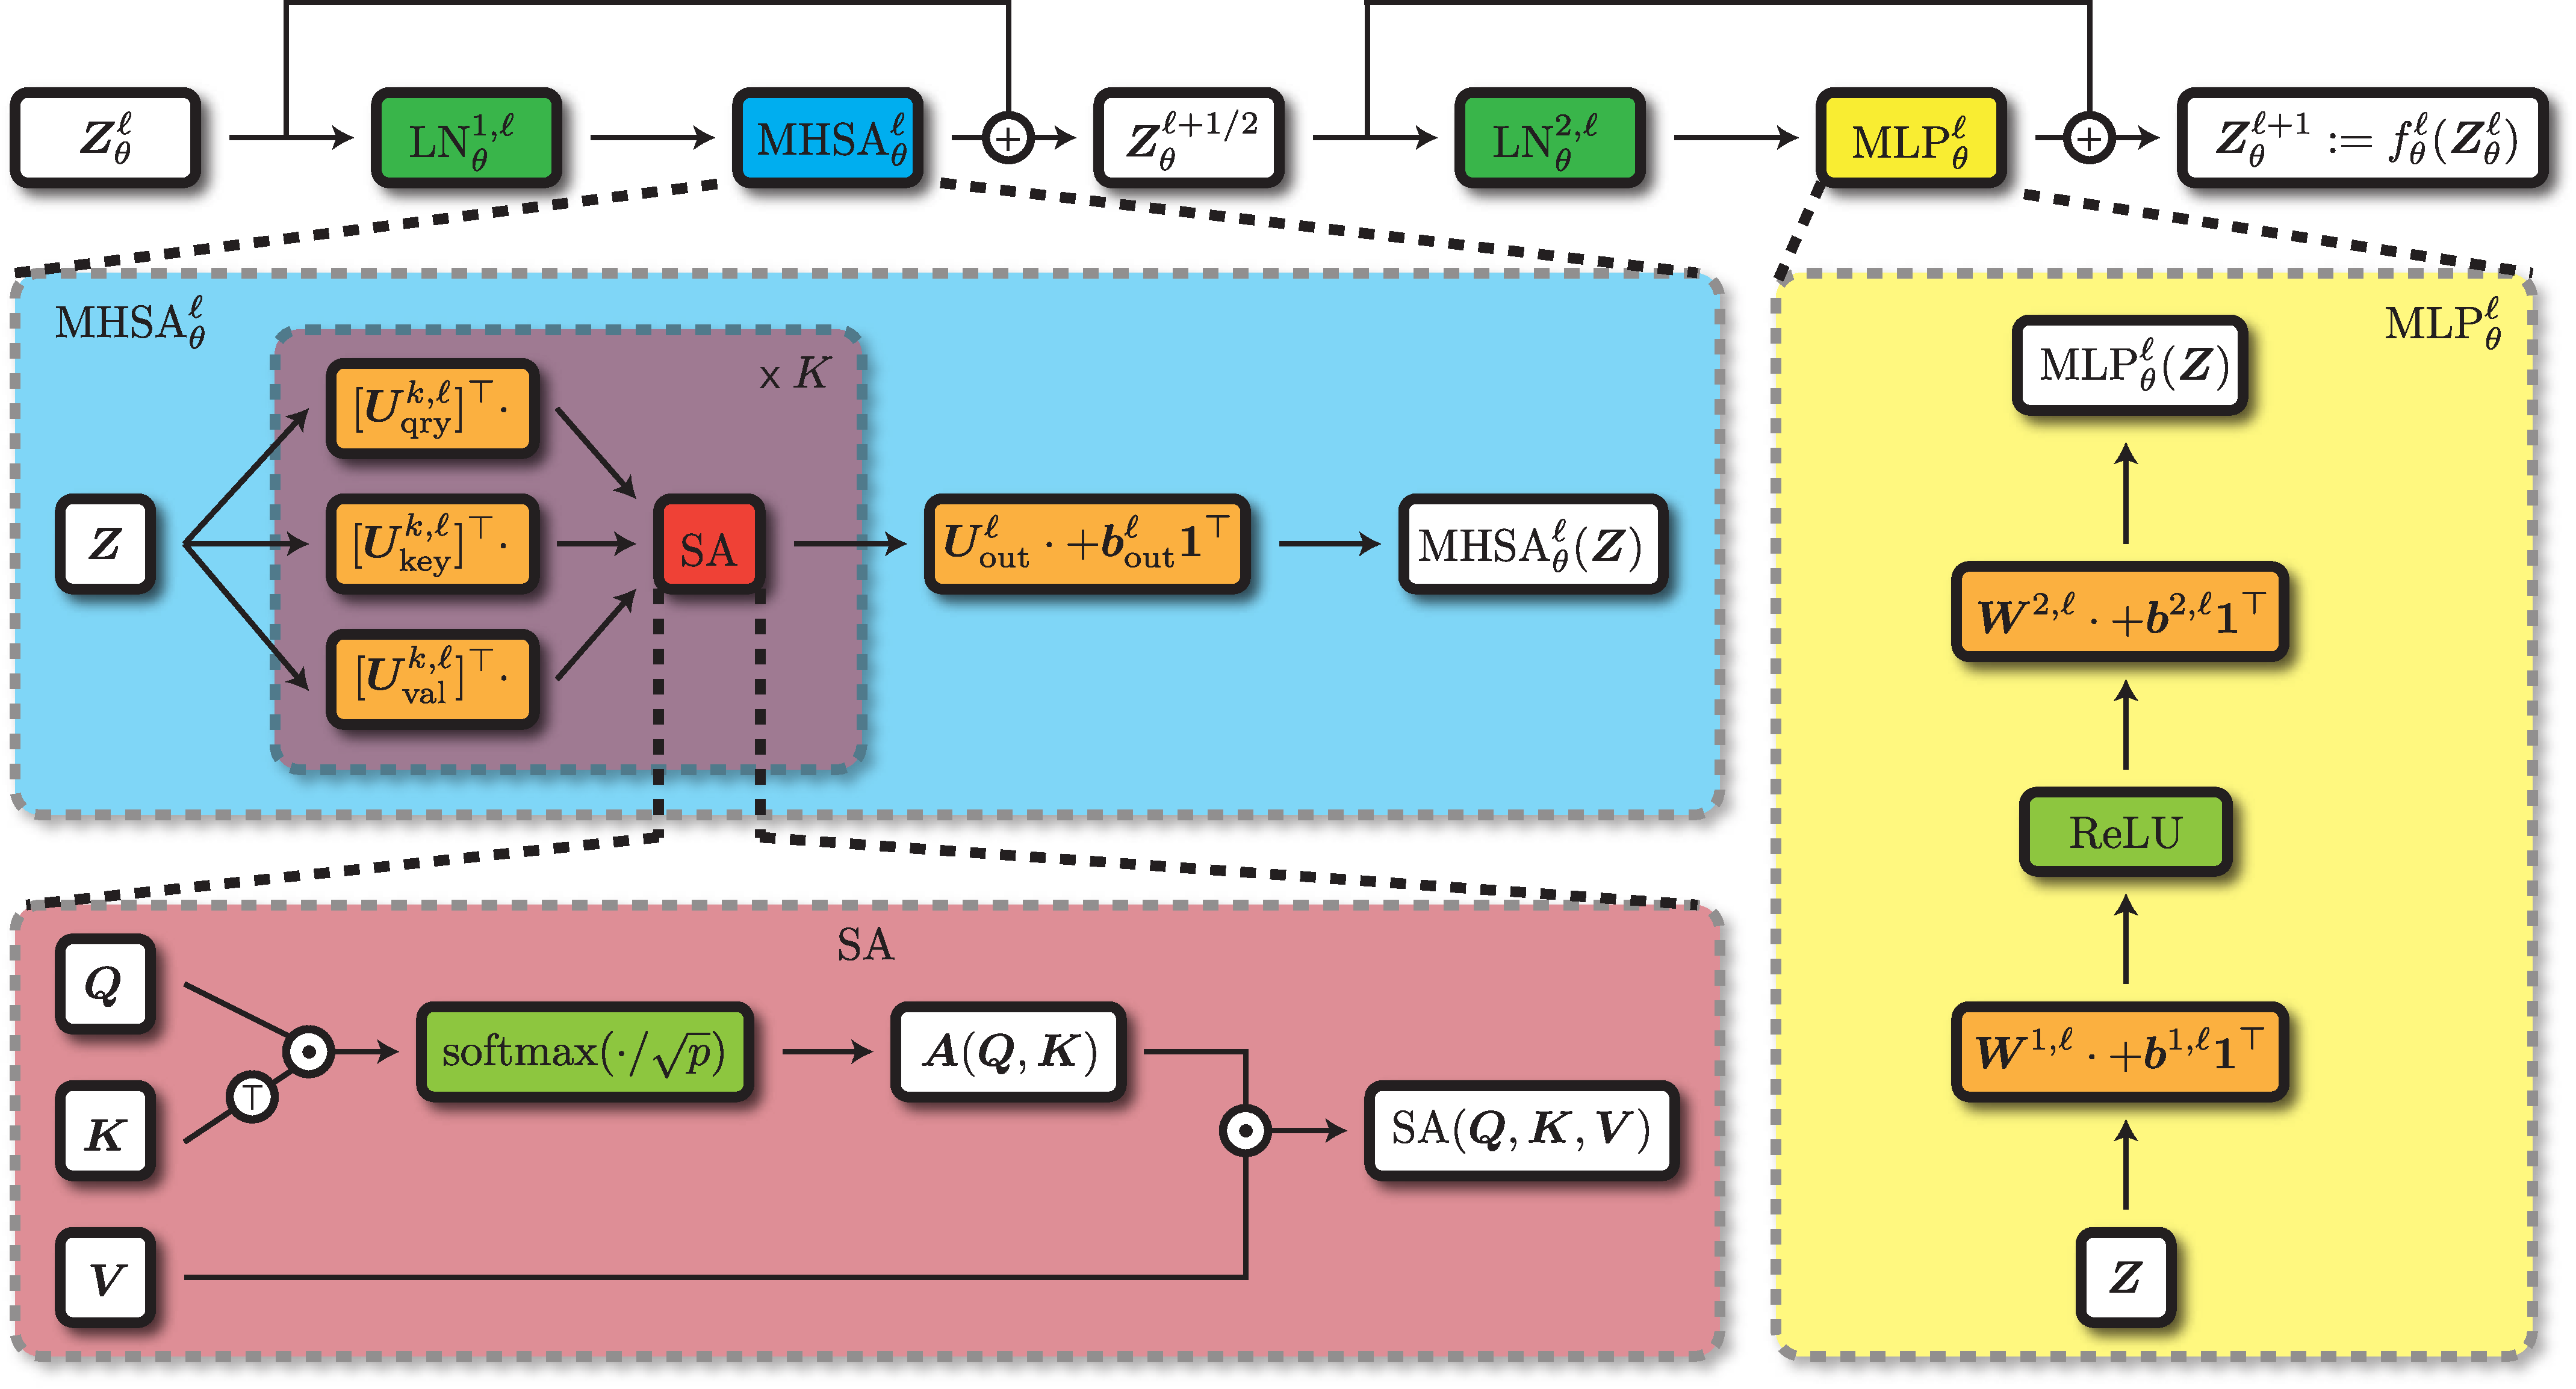
\includegraphics[width=\textwidth]{\toplevelprefix/chapters/chapter7/figs/transformer_backbone.pdf}
    \caption{\small\textbf{Transformer 主干网络的一层 \(f_{\theta}^{\ell}\)。} 输入特征依次通过层归一化、多头自注意力和多层感知机模块,形成该层的输出特征。}
    \label{fig:transformer_backbone}
\end{figure}

\paragraph{主干网络(Backbone)。} 给定一个嵌入序列 \(\vZ_{\theta}^{1}(\vX) := f_{\theta}^{\emb}(\vX) \in (\R^{d})^{*}\),我们使用主干网络映射 \(f_{\theta}^{\backbone}\) 对其进行处理,如下所示,并如 \Cref{fig:transformer_backbone} 所示。函数 \(f_{\theta}^{\backbone}\) 由 \(L\) 个\textit{层} \(f_{\theta}^{\ell}\) 组成,即
\begin{equation}
    f_{\theta}^{\backbone} = f_{\theta}^{L} \circ \cdots \circ f_{\theta}^{1}.
\end{equation}
 层 \(f_{\theta}^{\ell}\) 的实现如下:
\begin{align}\label{eq:vit-res-block}
    \vZ_{\theta}^{\ell + 1/2}(\vX)
    &= \vZ_{\theta}^{\ell}(\vX) + \MHSA_{\theta}^{\ell}(\LN_{\theta}^{1, \ell}(\vZ_{\theta}^{\ell}(\vX))) \\ 
    \vZ_{\theta}^{\ell + 1}(\vX)
    &= \vZ_{\theta}^{\ell + 1/2}(\vX) + \MLP_{\theta}^{\ell}(\LN_{\theta}^{2, \ell}(\vZ_{\theta}^{\ell + 1/2}(\vX)))
\end{align}
并且 \(f_{\theta}^{\ell}\) 的定义使得 \(f_{\theta}^{\ell}(\vZ_{\theta}^{\ell}(\vX)) := \vZ_{\theta}^{\ell + 1}(\vX)\)。这里我们使用了一些算子,如 \(\MHSA_{\theta}^{\ell}, \MLP_{\theta}^{\ell}\) 和 \(\LN_{\theta}^{i, \ell}\),它们的定义如下:
\begin{itemize}
    \item \(\MHSA_{\theta}^{\ell}\) 算子是多头自注意力(multi-head-self-attention),它是多头子空间自注意力(multi-head subspace self-attention,参见 \Cref{ch:representation})的前身。其公式如下:
    \begin{align}
        \MHSA_{\theta}^{\ell}(\vZ) \label{eq:mhsa}
        &:= \vU_{\out}^{\ell}\mat{\SA([\vU_{\query}^{1, \ell}]^{\top}\vZ, [\vU_{\key}^{1, \ell}]^{\top}\vZ, [\vU_{\val}^{1, \ell}]^{\top}\vZ) \\ \vdots \\ \SA([\vU_{\query}^{K, \ell}]^{\top}\vZ, [\vU_{\key}^{K, \ell}]^{\top}\vZ, [\vU_{\val}^{K, \ell}]^{\top}\vZ)} + \vb_{\out}^{\ell}\vone_{n}^{\top}, \\
        \label{eq:self_attention}
        \text{其中} \qquad \SA(\vQ, \vK, \vV)
        &:= \vV \underbrace{\softmax\rp{\frac{\vK^{\top}\vQ}{\sqrt{p}}}}_{:= \vA(\vQ, \vK)}
    \end{align}
    其中 \(p\) 是一个正整数,\(\vU_{\query}^{k, \ell}, \vU_{\key}^{k, \ell}, \vU_{\val}^{k, \ell} \in \R^{d \times p}\),\(\vU_{\out}^{\ell} \in \R^{d \times Kp}\) 和 \(\vb_{\out}^{\ell} \in \R^{d}\) 是包含在参数集 \(\theta\) 中的可训练参数,而 \(\softmax\) 是按列定义的,即
    \begin{align}
        \softmax(\vM) 
        &:= \mat{\softmax(\vm_{1}) & \cdots & \softmax(\vm_{p})}, \\ 
        \forall \vM 
        &= \mat{\vm_{1}, \dots, \vm_{p}} \in \R^{n \times p}.
    \end{align}
    在实践中,维度通常被选择为 \(Kp = d\)。项
    \begin{equation}
        \label{eq:attention_map}
        \vA_{\theta}^{k, \ell}(\vZ) := \vA([\vU_{\query}^{k, \ell}]^{\top}\vZ, [\vU_{\key}^{k, \ell}]^{\top}\vZ), \qquad \SA_{\theta}^{k, \ell}(\vZ) := \SA([\vU_{\query}^{k, \ell}]^{\top}\vZ, [\vU_{\key}^{k, \ell}]^{\top}\vZ, [\vU_{\val}^{k, \ell}]^{\top}\vZ)
    \end{equation}
    也分别被称为第 \(\ell\) 层的\textit{第 \(k\) 个注意力图}(attention map)和\textit{第 \(k\) 个注意力头输出}(attention head output)。此外,操作 \(\SA(\vQ, \vK, \vV)\) 可以使用专门的软件如 FlashAttention \citep{shah2025flashattention} 极其高效地计算。
    \item \(\MLP_{\theta}^{\ell}\) 是一个两层感知机,是深度网络中常用的非线性单元,其形式为
    \begin{equation}
        \MLP_{\theta}^{\ell}(\vZ) := \vW_{\down}^{\ell}\ReLU(\vW_{\up}^{\ell}\vZ + \vb_{\up}^{\ell}\vone_{n}^{\top}) + \vb_{\down}^{\ell}\vone_{n}^{\top}
    \end{equation}
    其中 \(\vW_{\up}^{\ell} \in \R^{q \times d}, \vW_{\down}^{\ell} \in \R^{d \times q}, \vb_{\up}^{\ell} \in \R^{q}, \vb_{\down}^{\ell} \in \R^{d}\) 是也包含在参数集 \(\theta\) 中的可训练参数,而 \(\ReLU\) 是逐元素的 ReLU 非线性函数,即 \(\ReLU(\vM)_{ij} = \max\{M_{ij}, 0\}\)。
    \item 每个层归一化(layer-norm)\(\LN_{\theta}^{i, \ell}\)(对于 \(i \in \{1, 2\}\))是一个标准的归一化操作,它独立地应用于每个词元特征的列:
    \begin{equation}
        \LN_{\theta}^{i, \ell}(\vZ) = \LN_{\theta}^{i, \ell}(\mat{\vz_{1}, \dots, \vz_{n}}) = \mat{\LN_{\theta}^{i, \ell}(\vz_{1}), \dots, \LN_{\theta}^{i, \ell}(\vz_{n})}
    \end{equation}
    其形式为
    \begin{equation}
        \LN_{\theta}^{i, \ell}(\vz) = \frac{\vz - \operatorname{mean}(\vz)\vone_{d}}{\norm{\vz - \operatorname{mean}(\vz)\vone_{d}}_{2}} \odot \valpha^{i, \ell} + \vbeta^{i, \ell} \qquad \text{其中} \qquad \operatorname{mean}(\vz) = \frac{1}{d}\vone_{d}^{\top}\vz
    \end{equation}
    其中 \(\odot\) 表示逐元素乘法,\(\valpha^{i, \ell}, \vbeta^{i, \ell} \in \R^{d}\) 是包含在参数集 \(\theta\) 中的可训练参数。层归一化算子对每个词元起到一种归一化作用,其后的每个词元的尺度是可学习的,并且在所有词元之间共享。
\end{itemize}

Transformer 是历史上最受欢迎的神经网络架构之一,为几乎所有深度学习领域的应用提供了动力。

\paragraph{特征提取器(Feature extractor)。} 我们使用一个后处理步骤 \(f_{\theta}^{\ext}\),它提取\textit{类别词元特征}(该特征,回想一下,旨在包含输入图像的聚合信息),并对其应用一个 MLP 和归一化。即,我们有
\begin{equation}
    \vz_{\theta}(\vX) := f_{\theta}^{\ext}(\vZ_{\theta}(\vX)) = f_{\theta}^{\ext}([\vz_{\theta}^{1}(\vX), \dots, \vz_{\theta}^{n}(\vX)]) := \frac{\MLP_{\theta}^{\ext}(\vz_{\theta}^{1}(\vX))}{\norm{\MLP_{\theta}^{\ext}(\vz_{\theta}^{1}(\vX))}_{2}}.
\end{equation} 

\paragraph{任务特定(“DINO”)头。} 对于 DINO,我们使用任务特定的 DINO 头 \(h_{\vW, \vmu}\)。对于 SimDINO,如前所述,我们\textit{完全不}使用任务特定头。

\subsection{优化策略}\label{sub:contrastive_learning_optimization}

\begin{figure}
    \centering 
    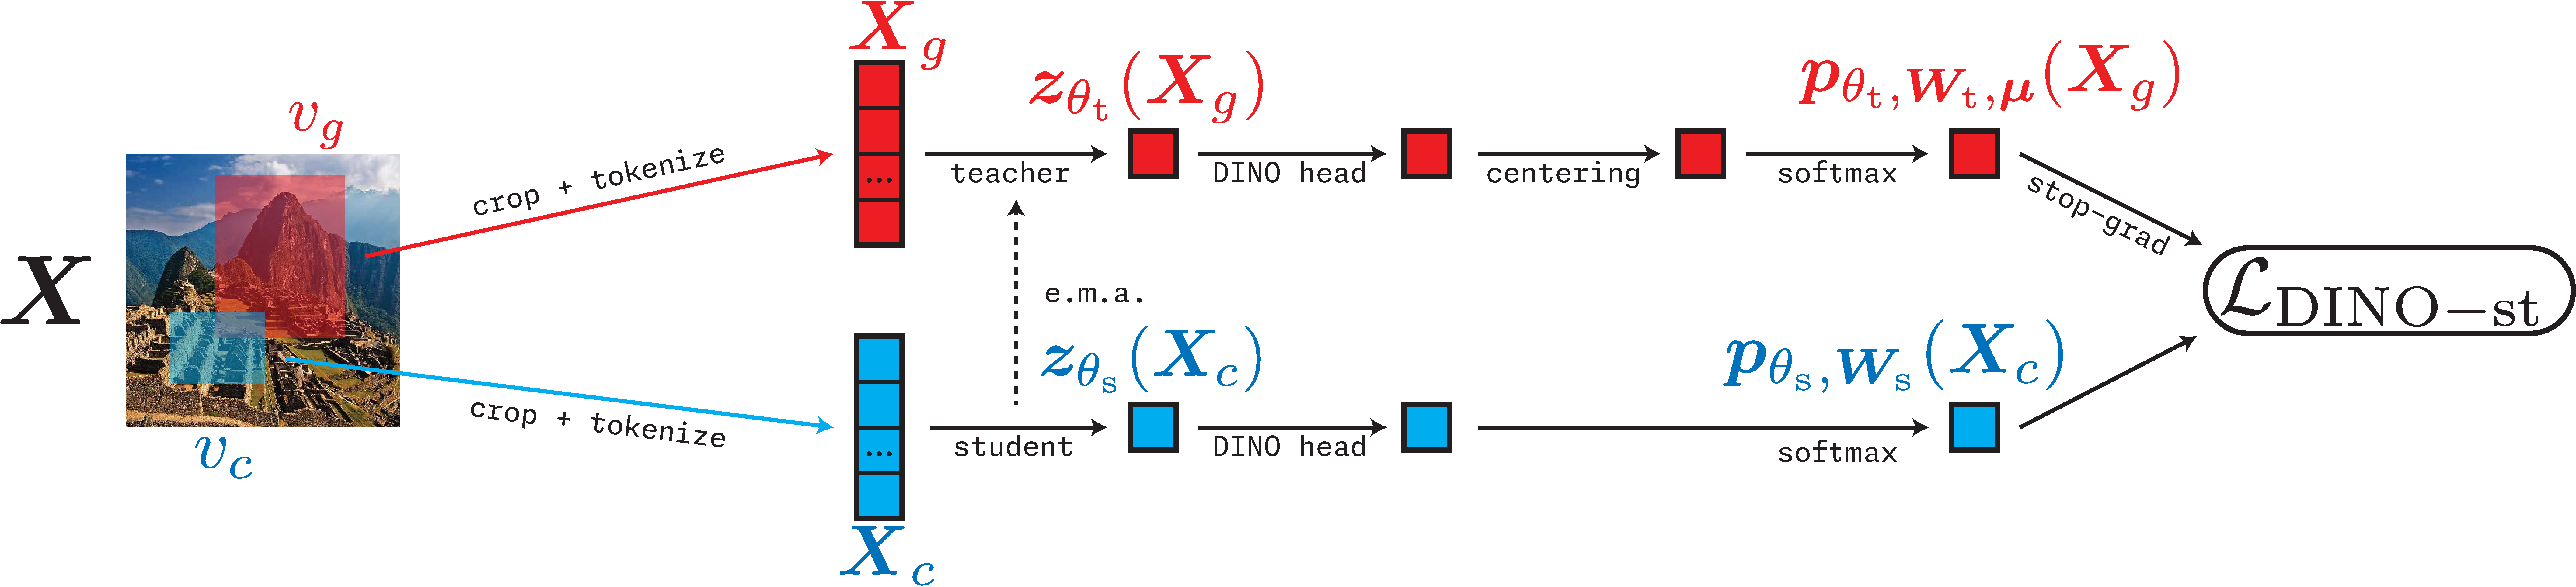
\includegraphics[width=\textwidth]{\toplevelprefix/chapters/chapter7/figs/dino_pipeline.pdf}
    \caption{\small \textbf{DINO 流程。} 为每个输入计算学生特征和教师特征。目标函数试图通过将两组特征投影到一个高维概率单纯形上并计算交叉熵损失来对齐学生特征和教师特征。值得注意的是,由于“停止梯度”(stop-grad),梯度仅相对于\textit{学生参数的输出}进行计算。}
    \label{fig:dino_pipeline}
\end{figure}

\paragraph{优化 DINO。} 我们有了损失函数和架构,现在我们来讨论优化策略。DINO 的优化策略使用\textit{两套权重用于同一架构}:\textit{学生}(student)权重 \(\theta_{\student}\) 和\textit{教师}(teacher)权重 \(\theta_{\teacher}\)。它们对应于两个具有相同架构的不同神经网络,分别称为教师网络和学生网络。教师网络编码所有全局视图,而学生网络编码所有“其他”视图。损失的目标是将教师的输出“蒸馏”到学生模型中。即,我们对损失 \(\cL_{\dino{}-\student\teacher}\) 进行训练:
\begin{equation}\label{eq:dino_loss_teacherstudent}
    \cL_{\dino{}-\student\teacher}(\theta_{\student}, \theta_{\teacher}, \vW_{\student}, \vW_{\teacher}, \vmu) := \Ex[d_{\CE}(\vp_{\theta_{\teacher}, \vW_{\teacher}, \vmu}(\vX_{g}), \vp_{\theta_{\student}, \vW_{\student}}(\vX_{c}))].
\end{equation}
现在,我们可以完整地描述 DINO 的整个流程,如 \Cref{fig:dino_pipeline} 所示。

虽然 \eqref{eq:dino_loss_teacherstudent} 很容易理解,但在实践中,用诸如梯度下降之类的优化算法来优化由 \(\cL_{\dino{}-\student\teacher}\) 给出的损失是不可能的。这是因为损失中的期望无法评估,更不用说求梯度了。在这种极其常见的情况下,我们通过有限样本来近似期望。也就是说,在每个时间步 \(k\),我们:
\begin{itemize}
    \item 从我们的数据集中子采样 \(B\) 个数据点 \(\{\vX_{1}^{(k)}, \dots, \vX_{B}^{(k)}\} \subset \cI\)。
    \item 对于每个数据点 \(\vX_{b}^{(k)}\),采样 \(M_{\glo}\) 个全局视图 \(v_{b, g}^{(k), i}\) 和 \(M_{\loc}\) 个局部视图 \(v_{b, \ell}^{(k), i}\)。将这些视图应用于 \(\vX_{b}^{(k)}\) 以获得 \(\vX_{b, g}^{(k), i} := v_{b, g}^{(k), i}(\vX_{b}^{(k)})\) 和 \(\vX_{b, \ell}^{(k), i} := v_{b, \ell}^{(k), i}(\vX_{b}^{(k)})\)。
    \item 对于每个\textit{局部}视图 \(\vX_{b, \ell}^{(k), i}\),计算以下量:
    \begin{equation}
        \vz_{\theta_{\student}}(\vX_{b, \ell}^{(k), i}) := (f_{\theta_{\student}}^{\ext} \circ f_{\theta_{\student}})(\vX_{b, \ell}^{(k), i}), \qquad \vp_{\theta_{\student}, \vW_{\student}}(\vX_{b, \ell}^{(k), i}) := h_{\vW_{\student}, \vzero_{m}}(\vz_{\theta_{\student}}(\vX_{b, \ell}^{(k), i}(\theta)))
    \end{equation}
    对于每个\textit{全局}视图 \(\vX_{b, g}^{(k), i}\),计算以下量(滥用一下符号):
    \begin{align}
        &\vz_{\theta_{\student}}(\vX_{b, g}^{(k), i}) := (f_{\theta_{\student}}^{\ext} \circ f_{\theta_{\student}})(\vX_{b, g}^{(k), i}), \qquad \vp_{\theta_{\student}, \vW_{\student}}(\vX_{b, g}^{(k), i}) := h_{\vW_{\student}, \vzero_{m}}(\vz_{\theta_{\student}}(\vX_{b, g}^{(k), i})), \\
        &\vz_{\theta_{\teacher}}(\vX_{b, g}^{(k), i}) := (f_{\theta_{\teacher}}^{\ext} \circ f_{\theta_{\teacher}})(\vX_{b, g}^{(k), i}), \qquad \vp_{\theta_{\teacher}, \vW_{\teacher}, \vmu}(\vX_{b, g}^{(k), i}) := h_{\vW_{\teacher}, \vmu}(\vZ_{\theta_{\teacher}}(\vX_{b, g}^{(k), i})).
    \end{align}
    \item 计算\textit{代理的、近似的损失} \(\hat{\cL}_{\dino-\student\teacher}^{(k)}\),定义如下:
    \begin{align}\label{eq:dino_loss_teacherstudent_empirical}
        &\hat{\cL}_{\dino{}-\student\teacher}^{(k)}(\theta_{\student}, \theta_{\teacher}, \vW_{\student}, \vW_{\teacher}, \vmu) :=
        \frac{1}{BM_{\glo}(M_{\glo} + M_{\loc} - 1)}\sum_{b = 1}^{B}\sum_{i = 1}^{M_{\glo}}\\
        &\Bigg[\sum_{j = 1}^{M_{\loc}}d_{\CE}(\vp_{\theta_{\teacher}, \vW_{\teacher}, \vmu}(\vX_{b, g}^{(k), i}), \vp_{\theta_{\student}, \vW_{\student}}(\vX_{b, \ell}^{(k), j})) + \sum_{\substack{j = 1 \\ j \neq i}}^{M_{\glo}}d_{\CE}(\vp_{\theta_{\teacher}, \vW_{\teacher}, \vmu}(\vX_{b, g}^{(k), i}), \vp_{\theta_{\student}, \vW_{\student}}(\vX_{b, g}^{(k), j}))\Bigg]\nonumber
    \end{align}
    以及它关于 \(\theta_{\student}\) 和 \(\vW_{\student}\) 的梯度,计算时应假设 \(\theta_{\teacher}\)、\(\vW_{\teacher}\) 和 \(\vmu\) 是常数——即它们与\textit{计算图分离},不依赖于 \(\theta_{\student}\) 和 \(\vW_{\student}\)。
    \item 通过迭代的、基于梯度的优化算法更新学生参数 \(\theta_{\student}\) 和 \(\vW_{\student}\),并通过指数移动平均(EMA)更新 \(\theta_{\teacher}\)、\(\vW_{\teacher}\) 和 \(\vmu\),衰减参数分别为 \(\nu^{(k)}\)、\(\nu^{(k)}\) 和 \(\rho^{(k)}\),即:
    \begin{align}
        (\theta_{\student}^{(k + 1)}, \vW_{\student}^{(k + 1)})
        &= \textsc{OptUpdate}^{(k)}(\theta_{\student}^{(k)}, \vW_{\student}^{(k)}; \nabla_{(\theta_{\student}, \vW_{\student})}\hat{\cL}_{\dino-\student\teacher}^{(k)}) \\
        \theta_{\teacher}^{(k + 1)}
        &= \nu^{(k)}\theta_{\teacher}^{(k)} + (1 - \nu^{(k)})\theta_{\student}^{(k + 1)} \\
        \vW_{\teacher}^{(k + 1)}
        &= \nu^{(k)}\vW_{\teacher}^{(k)} + (1 - \nu^{(k)})\vW_{\student}^{(k + 1)} \\
        \vmu^{(k + 1)}
        &= \rho^{(k)}\vmu^{(k)} + (1 - \rho^{(k)})\cdot\frac{1}{BM_{\glo}}\sum_{b = 1}^{B}\sum_{i = 1}^{M_{\glo}}\vW^{(k)}\vz_{\theta_{\teacher}}(\vX_{b, g}^{(k), i}),
    \end{align}
    例如,如果选择的优化算法是随机梯度下降,我们将有更新 \(\theta_{\student}^{(k + 1)} := \theta_{\student}^{(k)} - \delta^{(k)}\nabla_{\theta_{\student}}\hat{\cL}_{\dino{}-\student\teacher}^{(k)}\),依此类推。
\end{itemize}
注意,这个优化过程相当不规则:尽管所有四个参数在每次迭代中都会改变,但只有两个是直接通过基于梯度的方法更新的。另外两个是通过指数移动平均更新的,并且在计算任何梯度时确实被当作常数处理。训练结束后,我们丢弃学生权重,使用教师权重作为我们训练好的网络 \(f\),因为经验表明这种指数移动平均可以稳定最终的模型(这个想法被称为 Polyak 平均或迭代平均)。

\(\nu\) 和 \(\rho\) 在优化轨迹中如何变化(即函数 \(k \mapsto \nu^{(k)}\) 和 \(k \mapsto \rho^{(k)}\))是超参数或设计决策,通常 \(\nu^{(1)} < 1\) 且 \(\lim_{k \to \infty}\nu^{(k)} = 1\),\(\rho\) 也类似。用于 DINO 头 \(h_{\vW, \vmu}\) 的温度超参数 \(\tau\) 在优化轨迹中也会变化(尽管这种依赖性没有明确标记)。

使用代理(“经验”)损失将我们难以处理的优化问题(如优化 \eqref{eq:dino_loss_teacherstudent} 中的损失)转化为一个可处理的随机优化问题,这几乎是世界上所有深度学习模型训练时运行的方式。一旦你看过一些例子,这种转换就变得极其自然,我们希望在本章中提供这些例子。

\begin{figure}
    \centering 
    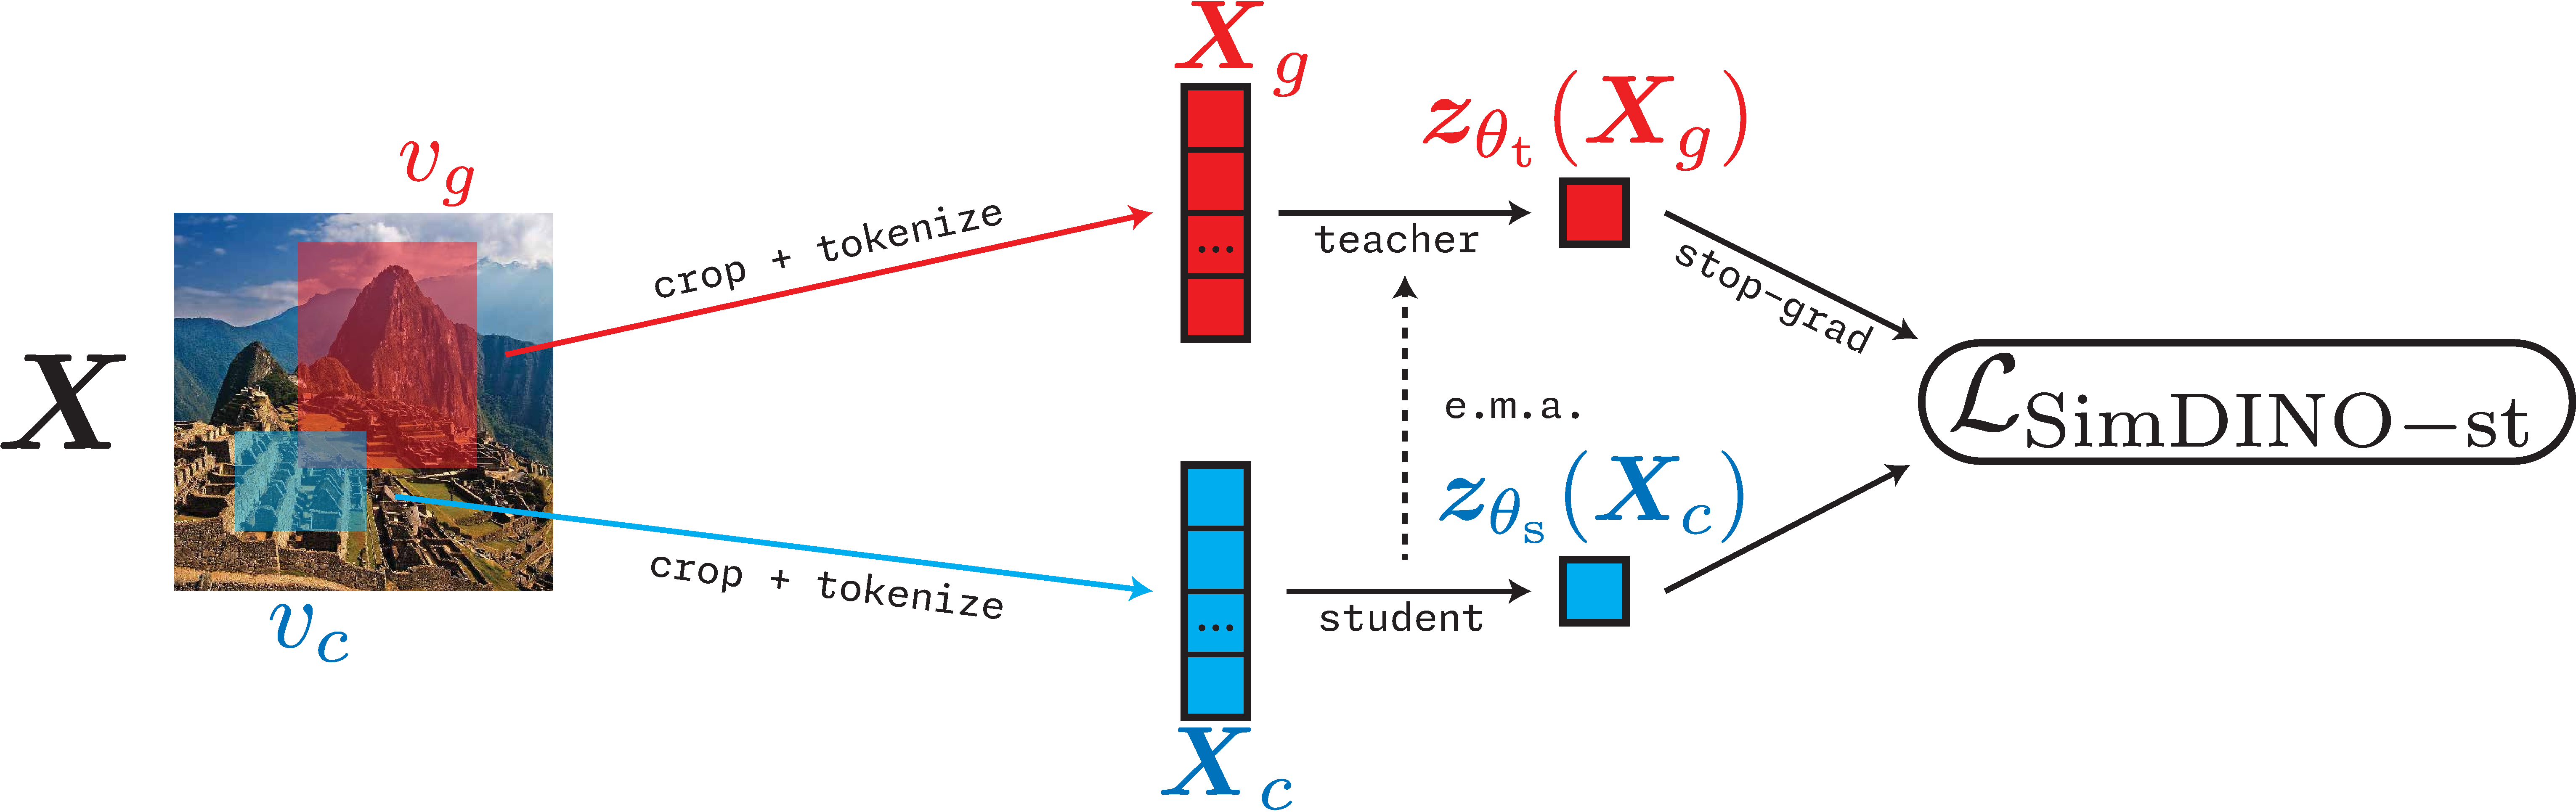
\includegraphics[width=0.7\textwidth]{\toplevelprefix/chapters/chapter7/figs/simdino_pipeline.pdf}
    \caption{\small\textbf{SimDINO 流程。} 与 \Cref{fig:dino_pipeline} 中的 DINO 流程相比,这里的损失是直接在特征上计算的,无需进一步操作。这省去了几个大矩阵的参数并简化了流程,同时使其训练更稳定。}\label{fig:simdino_pipeline}
\end{figure}

\paragraph{优化 SimDINO。} 简化的 DINO 总体层面上的目标在精神上非常相似,但在执行上简单得多,即:
\begin{equation}\label{eq:simdino_loss_teacherstudent}
    \cL_{\simdino-\student\teacher}(\theta_{\student}, \theta_{\teacher}) :=  \Ex\rs{d_{\ell^{2}}(\vz_{\theta_{\teacher}}(\vX_{g}), \vz_{\theta_{\student}}(\vX_{c}))} - \frac{\gamma}{2}\logdet\rp{\vI + \frac{d}{\eps^{2}}\Cov(\vz_{\theta_{\student}}(\vX_{g})))}.
\end{equation}
因此,如 \Cref{fig:simdino_pipeline} 中所阐述的,SimDINO 流程严格来说比 DINO 流程更简单。我们可以使用一个简化版的 DINO 训练流程来优化 SimDINO。在每个时间步 \(k\),我们:
\begin{itemize}
    \item 从我们的数据集中子采样 \(B\) 个数据点 \(\{\vX_{1}^{(k)}, \dots, \vX_{B}^{(k)}\} \subset \cI\)。
    \item 对于每个数据点 \(\vX_{b}^{(k)}\),采样 \(M_{\glo}\) 个全局视图 \(v_{b, g}^{(k), i}\) 和 \(M_{\loc}\) 个局部视图 \(v_{b, \ell}^{(k), i}\)。将这些视图应用于 \(\vX_{b}^{(k)}\) 以获得 \(\vX_{b, g}^{(k), i} := v_{b, g}^{(k), i}(\vX_{b}^{(k)})\) 和 \(\vX_{b, \ell}^{(k), i} := v_{b, \ell}^{(k), i}(\vX_{b}^{(k)})\)。
    \item 对于每个\textit{局部}视图 \(\vX_{b, \ell}^{(k), i}\),计算 \(\vz_{\theta_{\student}}(\vX_{b, \ell}^{(k), i}) := (f_{\theta_{\student}}^{\ext} \circ f_{\theta_{\student}})(\vX_{b, \ell}^{(k), i})\)。对于每个\textit{全局}视图 \(\vX_{b, g}^{(k), i}\),计算 \(\vz_{\theta_{\student}}(\vX_{b, g}^{(k), i}) := (f_{\theta_{\student}}^{\ext} \circ f_{\theta_{\student}})(\vX_{b, g}^{(k), i})\) 和 \(\vz_{\theta_{\teacher}}(\vX_{b, g}^{(k), i}) := (f_{\theta_{\teacher}}^{\ext} \circ f_{\theta_{\teacher}})(\vX_{b, g}^{(k), i})\)。
    \item 计算\textit{代理的、近似的损失} \(\hat{\cL}_{\simdino-\student\teacher}^{(k)}\),定义如下:
    \begin{align}\label{eq:simdino_loss_teacherstudent_empirical}
        &\hat{\cL}_{\simdino{}-\student\teacher}^{(k)}(\theta_{\student}, \theta_{\teacher}) :=
        \frac{1}{BM_{\glo}(M_{\glo} + M_{\loc} - 1)}\sum_{b = 1}^{B}\sum_{i = 1}^{M_{\glo}}\Bigg[\sum_{j = 1}^{M_{\loc}}d_{\ell^{2}}(\vz_{\theta_{\teacher}}(\vX_{b, g}^{(k), i}), \vz_{\theta_{\student}}(\vX_{b, \ell}^{(k), j})) \\ 
        &\qquad \qquad + \sum_{j = 1}^{M_{\glo}}d_{\ell^{2}}(\vz_{\theta_{\teacher}}(\vX_{b, g}^{(k), i}), \vz_{\theta_{\student}}(\vX_{b, g}^{(k), j}))\Bigg] - \frac{\gamma}{M_{\glo}}\sum_{i = 1}^{M_{\glo}}R_{\eps}([\vz_{\theta_{\student}}(\vX_{1, g}^{(k), i}), \dots, \vz_{\theta_{\student}}(\vX_{B, g}^{(k), i})])\nonumber
    \end{align}
    其中 \(R_{\eps}\) 是在有限样本上估计的高斯编码率,在 \Cref{ch:representation} 中有描述。 \(\hat{\cL}_{\simdino-\student\teacher}^{(k)}\) 关于 \(\theta_{\student}\) 的梯度应该(再次)在假设 \(\theta_{\teacher}\) 是常数的情况下计算。
    \item 通过迭代的、基于梯度的优化算法更新学生参数 \(\theta_{\student}\),并通过指数移动平均更新 \(\theta_{\teacher}\),衰减参数为 \(\nu^{(k)}\),即:
    \begin{align}
        \theta_{\student}^{(k + 1)}
        &= \textsc{OptUpdate}^{(k)}(\theta_{\student}^{(k)}; \nabla_{\theta_{\student}}\hat{\cL}_{\simdino-\student\teacher}^{(k)}) \\
        \theta_{\teacher}^{(k + 1)}
        &= \nu^{(k)}\theta_{\teacher}^{(k)} + (1 - \nu^{(k)})\theta_{\student}^{(k + 1)}.
    \end{align}
\end{itemize}
再次重申,梯度仅相对于 \(\theta_{\student}\) 计算,将 \(\theta_{\teacher}\) 视为常数。这里,请注意,虽然 \(\nu\) 的选择仍然是一个设计决策,但超参数 \(\rho\) 和 \(\tau\) 已被移除。


\subsection{评估方法}\label{sub:contrastive_learning_evals}
有几种方法可以评估一个训练好的 Transformer 模型。本节我们重点介绍两种。让我们定义\textit{中心裁剪}(center crop)视图 \(v_{\cc} \colon \cI \to \cI\),它是一个\textit{确定性的缩放裁剪}:
\begin{itemize}
    \item 它将图像缩放,使得最短边的大小为 \(S_{\rsz}\)(类似于面积百分比参数为 \(1\) 的随机缩放裁剪);
    \item 然后它取\textit{中心}的 \(S_{\cc} \times S_{\cc}\) 裁剪;
\end{itemize}
这样最终的形状是 \((C, S_{\cc}, S_{\cc})\)。注意,给定一个输入,视图 \(v_{\cc}\) 是完全确定性的。对于一个输入 \(\vX\),我们记 \(\vX_{\cc} := v_{\cc}(\vX)\)。这里 \(S_{\cc} \leq S_{\rsz}\)。


\paragraph{线性探查(Linear probing)。}

评估编码器模型 \(\vX \mapsto \vz_{\theta}(\vX)\) 的第一种,也是最与架构无关的方法,是采用\textit{线性探查}。简而言之,线性探查是在编码器计算出的聚合特征上运行逻辑回归。这告诉我们表示中存在多少语义信息,以及这些信息有多容易被提取。(也就是说:具有不同语义的图像的特征在多大程度上位于特征空间的不同子空间上?)

更正式地,假设我们想在图像-标签数据 \((\vX, \vy)\) 上评估编码器特征的质量和忠实度,其中有 \(N_{\cls}\) 个类别,\(\vy \in \{0, 1\}^{N_{\cls}}\) 是一个“独热编码”(即,如果 \(\vX\) 属于第 \(i\) 类,则在第 \(i\) 个位置为 \(1\),其他位置为 \(0\))。一种方法是解决逻辑回归问题
\begin{equation}\label{eq:linear_probing}
    \min_{\vW \in \R^{N_{\cls} \times d}}\Ex[\CE(\vy, \vW \vz_{\theta}(\vX_{\cc}))].
\end{equation}
更实际地,如果我们有带标签的数据 \(\{(\vX_{b}, \vy_{b})\}_{b = 1}^{B}\),我们可以解决\textit{经验}逻辑回归问题(类似于 \eqref{eq:dino_loss_teacherstudent} vs.~\eqref{eq:dino_loss_teacherstudent_empirical})
\begin{equation}\label{eq:linear_probing_empirical}
    \min_{\vW \in \R^{N_{\cls} \times d}}\frac{1}{B}\sum_{b = 1}^{B}\CE(\vy_{b}, \vW \vz_{\theta}(\vX_{b, \cc})).
\end{equation}
这个问题在 \(\vW\) 上是一个凸优化问题,因此可以通过(随机)梯度下降或一系列其他算法高效解决。这个线性探查器与编码器一起可以用作分类器,我们可以评估其分类准确率。通常的做法是,首先在一个大数据集(如 ImageNet-1K)上训练模型,然后在一个数据集(如 CIFAR-10 的训练集)上训练线性探查器,最后在一个与第二个数据集同分布的第三个(“留出”)数据集(如 CIFAR-10 的评估集)上进行评估。

\paragraph{\(k\)-近邻(\(k\)-nearest neighbors)。}  我们也可以通过使用 \(k\)-近邻算法来获得平均预测标签,从而评估特征在分类任务上的性能,而\textit{无需显式地训练一个分类器}。也就是说,给定一个数据集 \(\{\vz_{b}\}_{b = 1}^{B} \subseteq \R^{d}\),定义另一个点 \(\vz \in \R^{d}\) 的 \(k\)-近邻为 \(\operatorname{NN}_{k}(\vz, \{\vz_{b}\}_{b = 1}^{B})\)。使用这个记法,我们可以计算预测标签 \(\hat{\vy}_{\theta}(\vX \mid \{(\vX_{b}, \vy_{b})\}_{b = 1}^{B})\) 为
\begin{equation}
    \hat{\vy}_{\theta}(\vX \mid \{(\vX_{b}, \vy_{b})\}_{b = 1}^{B}) = \vone(i^{\star}) \quad \text{其中} \quad i^{\star} := \argmax_{i \in [Q]}\sum_{b = 1}^{B}\vy_{b}\indvar[\vz_{\theta}(\vX_{\cc, b}) \in \operatorname{NN}_{k}(\vz_{\theta}(\vX_{\cc}))].
\end{equation}
这里,\(\vone(i) \in \Delta_{N_{\cls}}\) 是(滥用一下符号,参见指示变量)在 \(i\) 处支撑的独热概率向量,即第 \(i\) 个坐标为 \(1\),其他为 \(0\)。也就是说,这个过程取特征空间中 \(k\) 个最近邻点中最常见的标签。\(k\)-近邻分类准确率就是这个预测标签的准确率,即
\begin{equation}
    \Ex_{\vX, \vy}[\indvar(\hat{\vy}_{\theta}(\vX \mid \{(\vX_{b}, \vy_{b})\}_{b = 1}^{B}) = \vy)]
\end{equation}
或者更常见的是其对应的经验版本,其中 \((\vX, \vy)\) 遍历一个有限的数据集(\textit{不是}用于 \(k\) 近邻的现有样本 \((\vX_{b}, \vy_{b})\))。

\paragraph{注意力图的保真度。}

对于基于 Transformer 的编码器,检查表示性能的另一种方法是检验在最后一层 \(L\) 的注意力图 \(\vA^{L, k} \in \R^{n \times n}\) 的保真度,该注意力图如 \Cref{eq:attention_map} 中定义,并通过以下流程给出:
\begin{align}
    \vX \mapsto \cdots \mapsto \vZ^{L - 1} = [\underbrace{\vz_{1}^{L - 1}}_{\text{类别词元}}, \underbrace{\vz_{2}^{L - 1} \dots, \vz_{n}^{L - 1}}_{\text{图像块词元}}] \mapsto \vA^{k, L} = \mat{\vA_{1, 1}^{k, L} & \vA_{1, 2:}^{k, L} \\ \vA_{2:, 1}^{k, L} & \vA_{2:, 2:}^{k, L}}.
\end{align}
特别地,我们检查对于给定的输入,注意力图揭示了输入图像中的哪些显著对象,即图像的哪些部分为类别词元提供了最全局相关的信息。一种特别的方法是检查注意力图的分量,其中类别词元被提取为查询(query),并从值(value)矩阵中移除,即 \(\vA_{2:, 1}^{k, L} \in \R^{1 \times (n - 1)} = \R^{1 \times N}\) 或其转置 \(\va^{k, L} = (\vA_{2:, 1}^{k, L})^{\top} \in \R^{N}\)。注意,这个我们标记为“第 \(L\) 层第 \(k\) 个注意力头的\textit{显著性向量}(saliency vector)”的向量 \(\va^{k, L}\),对每个图像块 \(1, \dots, N\) 都有一个值,我们用这个值来描述每个图像块对全局信息的相关性。特别地,为了可视化的目的,我们创建一幅新图像,其中每个图像块被其在显著性向量中对应的值所取代,从而展示每个图像块的贡献;我们称这幅图像为“第 \(L\) 层第 \(k\) 个注意力头的\textit{显著性图}(saliency map)”。为了可视化每个图像块对所有头的全局信息的总相关性,我们可以对显著性向量进行平均,即 \(\tilde{\va}^{L} := \frac{1}{K}\sum_{k = 1}^{K}\va^{k, L}\),并展开成\textit{平均显著性图}。平均显著性图应该能高亮输入图像的相关部分。


\paragraph{目标检测与分割。}

我们可以通过将表示用于\textit{语义分割}(semantic segmentation)来评估它们捕捉输入细粒度(即更小或更详细)属性的能力。粗略地说,这意味着我们使用特征来为输入中的所有对象构建边界框。有几种方法可以做到这一点,也有几种方法可以根据真实标签来评分得到的边界框。每种方法的组合对应于一个特定的分割度量。我们不在这里正式描述它们,因为它们并非特别具有启发性,但 DINO 论文 \citep{caron2021emerging} 和 DINOv2 论文 \citep{oquab2023dinov2} 包含了对实践中使用的所有度量的引用。

\subsection{实验设置与结果} \label{sub:contrastive_learning_experiment_results}

由于 SimDINO 是直接建立在 DINO 之上的,我们将 DINO 原始论文 \citep{caron2021emerging} 中给出的 DINO 最佳设置与应用于 SimDINO 的相同设置进行比较,以实现公平对比。

\paragraph{目标函数。} 在所有实验中,我们使用 \(10\) 个分辨率为 \(96 \times 96\) 的局部视图(即 \(M_{\loc} = 10\),\(S_{\loc} = 96\))和 \(2\) 个分辨率为 \(224 \times 224\) 的全局视图(即 \(M_{\glo} = 2\),\(S_{\glo} = 224\))。为局部和全局视图裁剪的原始图像部分的比例分别为 \(p_{\loc} \in [\frac{1}{20}, \frac{3}{10}]\) 和 \(p_{\glo} \in [\frac{3}{10}, 1]\)(每个视图随机选择)。缩放后裁剪区域内的较短边尺寸为 \(S_{\rsz} = 256\),中心裁剪(评估)视图的边长为 \(S_{\cc} = 224\)。所有这些设置都适用于 DINO 和 SimDINO。

\paragraph{模型架构。} 对于所有输入,我们将图像块大小设置为 \(16 \times 16\)(即 \(P_{H} = P_{W} = 16\))。我们使用 ViT \citep{dosovitskiy2020image} 架构的小型、基础和大型模型作为嵌入层和主干网络。特征提取器是一个三层 MLP,隐藏层大小为 \(2048\),输出维度为 \(256\),后接一个 \(\ell^{2}\)-归一化,如 \Cref{sub:contrastive_learning_architecture} 中所述。对于 DINO 架构(即非 SimDINO 架构),DINO 头 \(\vW\) 是一个 \(\R^{65536 \times 256}\) 的矩阵,参数 \(\vmu\) 是一个 \(\R^{65536}\) 的向量。

\paragraph{数据集与优化。} 对于预训练,我们的 DINO 复现和 SimDINO 在所有方法中都使用 ImageNet-1K 数据集。我们使用 AdamW \citep{Loshchilov2017DecoupledWD} 作为优化器,这是一个非常标准的选择。我们遵循以下超参数建议:
\begin{itemize}
    \item 批处理大小为 \(B = 1024\)。
    \item 学习率(对于 AdamW 和学生模型)的“基础”值为 \(2 \times 10^{-3}\)。在前 \(10\) 个周期(epoch)中,学习率从 \(0\) 线性增加到基础值(即,在第 \(i\) 个周期,学习率为 \((i/10) \cdot 2 \times 10^{-3}\),对于 \(1 \leq i \leq 10\))。然后在接下来的 \(90\) 个周期中,学习率通过所谓的\textit{余弦调度}(cosine schedule)衰减回 \(0\)。余弦调度的定义在许多地方都有给出,包括 \href{https://pytorch.org/docs/stable/generated/torch.optim.lr_scheduler.CosineAnnealingLR.html}{PyTorch 文档},它在训练深度视觉模型时常用。
    \item 权重衰减(AdamW 中的 W)在训练过程中遵循从 0.04 到 \(0.4\) 的余弦调度。
    \item EMA 率 \(\nu\) 在训练过程中遵循从 \(0.996\) 到 \(1.0\) 的余弦调度。特别对于 DINO,中心化 EMA 率 \(\rho\) 固定为 \(0.9\)。
    \item 特别对于 DINO,教师温度 \(\tau_{\teacher}\) 固定为 \(0.1\),而学生温度 \(\tau_{\student}\) 在前 \(30\) 个周期内从 \(0.04\) 线性增加到 \(0.07\),之后固定为 \(0.07\)。
\end{itemize}
在训练期间,对于看到的每张图像,在进行局部和全局视图裁剪之前,我们使用一些(基本上是信息保持的)数据增强,如翻转、颜色抖动、高斯模糊和日晒效果。控制这些增强的确切超参数在此处未列出,但在 DINO 论文 \citep{caron2021emerging} 中有引用。

对于线性探查,线性探查器通常使用 AdamW 优化器进行训练,学习率为 \(2 \times 10^{-4}\),权重衰减为 \(0.01\),批处理大小为 \(512\),但这些参数通常会根据具体情况进行修改以最小化损失。


\begin{table}
    \centering
    \begin{tabular}{@{}lcccc@{}} % Removed extra horizontal padding
        \toprule
        方法 & 模型 & 周期数 & 20-NN & 线性探查
        \\
        \midrule 
        DINO & ViT-B & 100 & 72.9 & 76.3 \\
        SimDINO & ViT-B & 100 & \bf 74.9 & \bf 77.3 \\
        DINO & ViT-L & 100 & -- & -- \\
        SimDINO & ViT-L & 100 & \bf 75.6 & \bf 77.4 \\
        \midrule
        \color{gray} SwAV & \color{gray} ViT-S & \color{gray} 800 & \color{gray} 66.3 & \color{gray} 73.5 \\
        \color{gray} MoCov3 & \color{gray} ViT-B & \color{gray} 300  & \color{gray} -- & \color{gray} 76.7 \\
        \bottomrule
    \end{tabular}
    \caption{\small\textbf{在留出测试数据上的分类性能},针对 DINO 和 SimDINO,使用 \(k\)-近邻准确率(\(k = 20\))和线性探查。在相同的迭代次数(\(100\))下,SimDINO 在性能上明显更优,并且更稳定(在 ViT-L 主干网络上使用所提供设置的 DINO 训练优化非常不稳定,很快就会得到 NaN 损失)。我们还与其他杰出方法进行了比较,即 DINO 所基于的 SwAV 和 MoCov3。}
    \label{tab:dino_imagenet_linear_probing}
\end{table}

\begin{figure}
    \centering 
    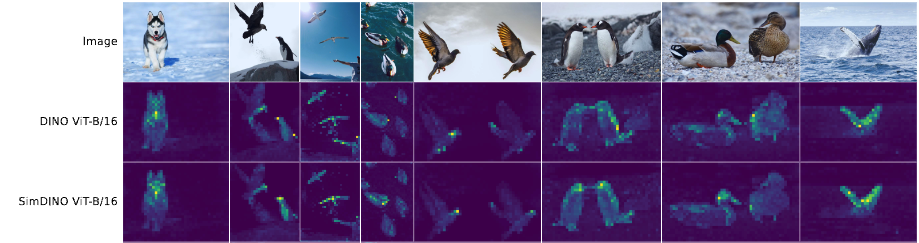
\includegraphics[width=\textwidth]{\toplevelprefix/chapters/chapter7/figs/dino_attention_maps.png}
    \caption{\small\textbf{由 DINO(\textit{中间行})和 SimDINO(\textit{底行})生成的显著性图的定性比较。} 对于每张图像,我们计算并显示最后一层 \(L\) 的平均显著性图。不同模型之间的显著性图相似,这意味着所有模型都收敛到关于哪些对象是重要的相似概念。请注意,尽管 \(X_{\evaluation}\) 是一张正方形图像,但为了进行此可视化,它被插值回矩形形状。}
    \label{fig:dino_attention_maps_saliency}
\end{figure}

\begin{table}
    \centering 
    \begin{tabular}{@{}llcccccccc@{}}
        \toprule
         &  & \multicolumn{3}{c}{检测 $\uparrow$} &  \multicolumn{3}{c}{分割 $\uparrow$} \\ 
        方法 & 模型 & AP$_{50}$  & AP$_{75}$ & AP & AP$_{50}$ & AP$_{75}$ & AP  \\ 
        \midrule
        SimDINO &ViT-L/16 &\bf 5.4 &1.9 &2.4 &4.5 &1.4 &1.9 \\
        SimDINO &ViT-B/16 &5.2 & \bf 2.0 & \bf 2.5 & \bf4.7 & \bf 1.5 & \bf 2.0 \\
        DINO &ViT-B/16 &3.9 &1.5 &1.8 &3.1 &1.0 &1.4 \\
        \midrule
        \color{gray} DINO & \color{gray} ViT-B/8 & \color{gray}5.1 & \color{gray}2.3 & \color{gray}2.5 & \color{gray}4.1 & \color{gray}1.3 & \color{gray}1.8 \\
        \bottomrule
    \end{tabular}
    \caption{\small\textbf{预训练的 DINO 和 SimDINO 模型在 COCO val2017 \citep{lin2014microsoft} 上的分割性能},这是一个包含对象位置元数据的分割数据集。我们不在 COCO 上进行训练,仅使用预训练的嵌入层和主干网络,边界框通过一种名为 MaskCut \citep{wang2023cut} 的方法从特征中提取。尽管如此,在公平比较下,SimDINO 在目标检测和分割方面超过了 DINO,甚至超过了使用更小图像块尺寸(边长为 \(8\) 而不是 \(16\))的 DINO。众所周知,较小的图像块尺寸有助于提高性能,尤其是在检测和分割任务中,因此这一结果相当令人惊讶和鼓舞。}
    \label{tab:dino_segmentation}
\end{table}

\paragraph{评估结果。} 在下游分类性能方面,我们获得了 \Cref{tab:dino_imagenet_linear_probing} 中的性能。我们观察到,在公平比较下,SimDINO 的性能远高于 DINO。而且,它要稳定得多:DINO 的规定设置无法训练 ViT-L(arge) 模型。另一方面,\Cref{fig:dino_attention_maps_saliency} 展示了 DINO 和我们简化的 SimDINO 中平均显著性图的可视化,观察到不同模型间的显著性图看起来非常相似,这表明这些模型学习到的特征在捕捉细粒度细节方面至少同样出色。\Cref{tab:dino_segmentation} 中的分割和目标检测性能从数量上证实了这一说法,其中 SimDINO 的特征显示出比 DINO 的特征有实质性的改进。



\section{图像分类}

\label{sec:image_classification}

在上一节中,我们从压缩的视角,运用表示学习的直觉,简化了一个过于复杂的学习目标。然而,许多最流行的学习过程却异常简单。在这些情况下,要进一步简化目标函数变得十分困难。因此,在本节及后续章节中,我们将专注于为各种任务寻找有原则的方法来修改\textit{深度网络架构}。

让我们首先从机器学习中最经典的任务——\textit{图像分类}——开始。这项任务常被用作评估模式识别算法或深度网络架构的标准任务。根据我们在\Cref{ch:representation}中对白盒架构的讨论,我们只需要一个有语义意义的任务,便能用白盒架构学习到良好的表示。我们将在本节中验证这一想法。

首先,数据集与\Cref{sub:contrastive_learning_data}中的基本保持一致。训练和测试数据都由带标签的图像组成,即图像-标签对\((\vX, \vy) \in \R^{C \times H \times W} \times \{0, 1\}^{N_{\cls}}\)。我们仍然对每个新批次中的每个样本应用各种数据增强(例如,翻转、高斯模糊、日晒效果等)。

\subsection{任务与目标} \label{sub:image_classification_objective}

与之前不同,我们的任务不仅是学习数据的良好表示,还要同时构建一个分类器。形式上,我们有带标签的数据对\((\vX, \vy)\),其中\(\vy \in \{0, 1\}^{N_{\cls}}\)是一个独热向量,表示\(\vX\)的类别归属。我们考虑输入数据\(\vX\)的一个确定性的\textit{中心裁剪视图}\(v_{\cc}\)(参见\Cref{sub:contrastive_learning_objective})。我们希望联合训练一个特征映射\((f_{\theta}, f_{\theta}^{\ext})\)和一个\textit{分类头}\(h_{\theta}\),定义如下:
\begin{equation}
    h_{\theta}(\vz) := \softmax(\vW^{\head}\vz + \vb^{\head}), \qquad  \forall \vz \in \R^{d}
\end{equation}
其中\((\vW^{\head}, \vb^{\head}) \in \R^{N_{\cls} \times d} \times \R^{N_{\cls}}\)是参数集\(\theta\)中的可训练参数,使得映射\(\vX_{\cc} \mapsto \vp_{\theta}(\vX_{\cc}) := h_{\theta}(\vz_{\theta}(\vX_{\cc}))\)能为输入\(\vX\)的视图\(\vX_{\cc} = v_{\cc}(\vX)\)预测一个平滑标签。该学习问题旨在最小化通过交叉熵度量的\(\vp_{\theta}\)与\(\vy\)之间的距离:
\begin{equation}\label{eq:classification_ce_loss}
    \min_{\theta}\bc{\cL_{\CE}(\theta) := \Ex[\CE(\vy, \vp_{\theta}(\vX_{\cc}))]}.
\end{equation}


\subsection{CRATE架构}\label{sub:image_classification_architecture}

我们使用的架构是CRATE架构,在\Cref{ch:representation}中有一定程度的详细描述。其总体设置与\Cref{sub:contrastive_learning_architecture}中的常规Transformer相似,但有几处改动。虽然嵌入步骤与\Cref{sub:contrastive_learning_architecture}中的DINO和SimDINO相同,特征提取步骤与\Cref{sub:contrastive_learning_architecture}中的SimDINO相同(因为它只提取与类别词元对应的特征),并且分类头在\Cref{sub:image_classification_objective}中有所描述,但其主干架构是不同的。每一层的形式如下:
\begin{align}\label{eq:CARTE updates}
    \vZ_{\theta}^{\ell + 1/2}(\vX)
    &= \vZ_{\theta}^{\ell}(\vX) + \MSSA_{\theta}^{\ell}(\LN_{\theta}^{1, \ell}(\vZ_{\theta}^{\ell}(\vX))), \\ 
    \vZ_{\theta}^{\ell + 1}(\vX)
    &= \ISTA_{\theta}^{\ell}(\LN_{\theta}^{2, \ell}(\vZ_{\theta}^{\ell + 1/2}(\vX))),
\end{align}
其中\(\MSSA_{\theta}^{\ell}\)和\(\ISTA_{\theta}^{\ell}\)块如\Cref{ch:representation}中所述,即:
\begin{itemize}
    \item \(\MSSA\)算子是多头子空间自注意力(multi-head-subspace-self-attention),定义如下:
    \begin{equation}
        \MSSA_{\theta}^{\ell}(\vZ) := \vU_{\out}^{\ell}\mat{\SA([\vU^{1, \ell}]^{\top}\vZ, [\vU^{1, \ell}]^{\top}\vZ, [\vU^{1, \ell}]^{\top}\vZ)\\ \vdots \\ \SA([\vU^{K, \ell}]^{\top}\vZ, [\vU^{K, \ell}]^{\top}\vZ, [\vU^{1, \ell}]^{\top}\vZ)} + \vb_{\out}^{\ell}\vone_{n}^{\top}
    \end{equation}
    其中\(\vU^{k, \ell} \in \R^{d \times p}\)、\(\vU_{\out}^{\ell} \in \R^{d \times Kp}\)和\(\vb_{\out}^{\ell} \in \R^{d}\)是属于参数集\(\theta\)的可训练参数,并且(回顾一下)自注意力算子\(\SA\)在\eqref{eq:self_attention}中定义。
    \item \(\ISTA\)算子是迭代收缩阈值算法(iterative-shrinkage-thresholding-algorithm)算子,定义如下:
    \begin{equation}
        \ISTA_{\theta}^{\ell}(\vZ) := \ReLU(\vZ - \beta (\vD^{\ell})^{\top}(\vD^{\ell}\vZ - \vZ) + \beta\lambda \vone_{d}\vone_{n}^{\top}),
    \end{equation}
    如此命名是因为映射\(\vX \mapsto \ReLU(\vX - \beta \vD^{\top}(\vD\vX - \vZ) + \beta  \lambda \vone_{d}\vone_{n}^{\top})\)是成熟的ISTA算法中的一步,该算法用于寻找\(\vZ\)关于完备字典\(\vD\)的元素级非负稀疏表示(参见\Cref{sec:dictionary_learning})。
\end{itemize}

我们将此架构称为CRATE,其主干的一层如图\Cref{fig:crate_backbone}所示。CRATE模型除了具有可解释性之外,通常还具有高性能和高参数效率。

\subsection{优化} \label{sub:image_classification_optimization}

我们使用一个简单的端到端随机优化过程来训练我们的分类器,在该过程中,我们对数据和视图进行子采样,计算这些样本上的平均损失及其梯度,并使用一个优化算法来改变参数。在每个时间步\(k\),我们:
\begin{itemize}
    \item 子采样\(B\)个不同的带标签样本\(\{(\vX_{b}^{(k)}, \vy_{b}^{(k)})\}_{b = 1}^{B} \subseteq \cI \times \{0, 1\}^{N_{\cls}}\)。
    \item 对每个带标签样本\((\vX_{b}^{(k)}, \vy_{b}^{(k)})\),计算中心裁剪视图\(v_{b, \cc}^{(k)}\)并将其应用于\(\vX_{b}^{(k)}\),得到\(\vX_{b, \cc}^{(k)} := v_{b, \cc}^{(k)}(\X_{b}^{(k)})\)。
    \item 计算预测值\(\vp_{\theta}(\vX_{b, \cc}^{(k)}) := (h_{\theta} \circ f_{\theta}^{\ext} \circ f_{\theta})(\vX_{b, \cc}^{(k)})\)。
    \item 构建代理随机损失
    \begin{equation}
        \hat{\cL}_{\CE}^{(k)}(\theta) := \frac{1}{B}\sum_{b = 1}^{B}\CE(\vy_{b}^{(k)}, \vp_{\theta}(\vX_{b, \cc}^{(k)})).
    \end{equation}
    \item 对\(\theta\)执行一步优化算法,得到以下迭代:
    \begin{equation}
        \theta^{(k + 1)} := \textsc{OptUpdate}^{(k)}(\theta^{(k)}; \nabla_{\theta}\hat{\cL}_{\CE}^{(k)}).
    \end{equation}
\end{itemize}


\subsection{评估方法} \label{sub:image_classification_evals}

我们使用与\Cref{sub:contrastive_learning_evals}相同的评估程序。总而言之,对于所有评估(以及训练),我们都使用一个中心裁剪视图\(v_{\cc}\),它将输入图像重塑并取一个大小为\((C, S_{\cc}, S_{\cc})\)的大中心裁剪,其中\(C\)是输入图像的通道数。然后,基于此视图的输出,我们可以进行线性探查、注意力图可视化以及检测/分割基准测试。

\subsection{实验设置与结果}\label{sub:image_classification_experiments}

由于CRATE直接基于Transformer,我们将\cite{dosovitskiy2020image,touvron2020training}给出的ViT的最优设置与应用于CRATE的相同设置进行比较,以实现公平对比。

\paragraph{模型架构。} 在评估和训练中,中心裁剪都先将整个图像缩放,使其较短的边长为\(256\)(即\(S_{\rsz} = 256\)),然后再进行\(224 \times 224\)大小的中心裁剪(即\(S_{\cc} = 224\))。我们采用的图像块大小为\(16\)(即\(P_{H} = P_{W} = 16\))。我们使用ViT \cite{dosovitskiy2020image}架构的tiny、small、base和large模型作为嵌入和主干,分别用MSSA和ISTA替换MHSA和MLP组件,在MSSA中保持相同的头数和头维度,从而大幅减少了训练参数的数量。对于CRATE,我们设置\((\beta, \lambda) = (1, 0.1)\)。

\paragraph{数据集与优化。} 对于预训练,我们使用ImageNet-1K数据集。我们使用LION优化器\citep{chen2024symbolic}来预训练我们的ViT复现模型以及CRATE。我们设置基础学习率为\(2.4 \times 10^{-4}\),权重衰减为\(0.5\),批处理大小为\(B = 2048\)。我们的学习率调度方案在前\(5\)个周期内将学习率线性增加至基础学习率,然后在接下来的\(145\)个周期内使用余弦调度将其降至\(0\)(所有模型均训练\(150\)个周期)。在预训练阶段,我们对图像数据应用常规的数据增强方案(翻转、高斯模糊、日晒效果等),并向标签中添加少量噪声(这被称为\textit{标签平滑}\citep{muller2019does})。

对于线性探查,我们使用多个评估数据集,如CIFAR10、Oxford-Flowers和Oxford-IIT-Pets。我们使用AdamW优化器来训练线性探查模型,学习率为\(5 \times 10^{-5}\),权重衰减为\(0.01\),批处理大小为\(B = 256\)。我们同样对图像数据应用前述的数据增强方法。

\begin{table}
    \centering
    \begin{tabular}{@{}lcccc|cc@{}}
    \toprule
    \textbf{模型} & CRATE-T  &  CRATE-S & CRATE-B & CRATE-L & { \color{gray} ViT-T} &  { \color{gray}ViT-S } \\ 
    \midrule
    \midrule
     \# 参数 & 6.09M & 13.12M & 22.80M & 77.64M & { \color{gray} 5.72M} & { \color{gray} 22.05M} \\
    \midrule
     ImageNet-1K & 66.7 & 69.2 & 70.8 & 71.3 & { \color{gray} 71.5} & { \color{gray} 72.4} \\
     ImageNet-1K ReaL & 74.0 & 76.0 & 76.5 & 77.4 & { \color{gray} 78.3 } & { \color{gray} 78.4} \\
    %  \midrule
     CIFAR10 & 95.5 & 96.0 & 96.8 & 97.2 & { \color{gray} 96.6} & { \color{gray} 97.2} \\
     CIFAR100 & 78.9 & 81.0 & 82.7 & 83.6 & { \color{gray} 81.8} & { \color{gray} 83.2}\\
     Oxford Flowers-102 & 84.6 & 87.1 & 88.7 & 88.3 & { \color{gray} 85.1} & { \color{gray} 88.5}\\
     Oxford-IIIT-Pets & 81.4 & 84.9 & 85.3 & 87.4 & { \color{gray} 88.5} & { \color{gray} 88.6} \\
     \bottomrule
    \end{tabular}
    \caption{\small \textbf{CRATE和ViT的线性探查分类准确率},在主干网络于ImageNet-1K上进行分类预训练后,于不同数据集和不同模型尺寸下的表现。我们观察到,在相同的模型配置下,CRATE以更简单、更有原则且参数效率更高的设计,取得了可比的分类性能。}
    \label{tab:crate_classification_linear_probing}
\end{table}

\begin{figure}
    \centering
    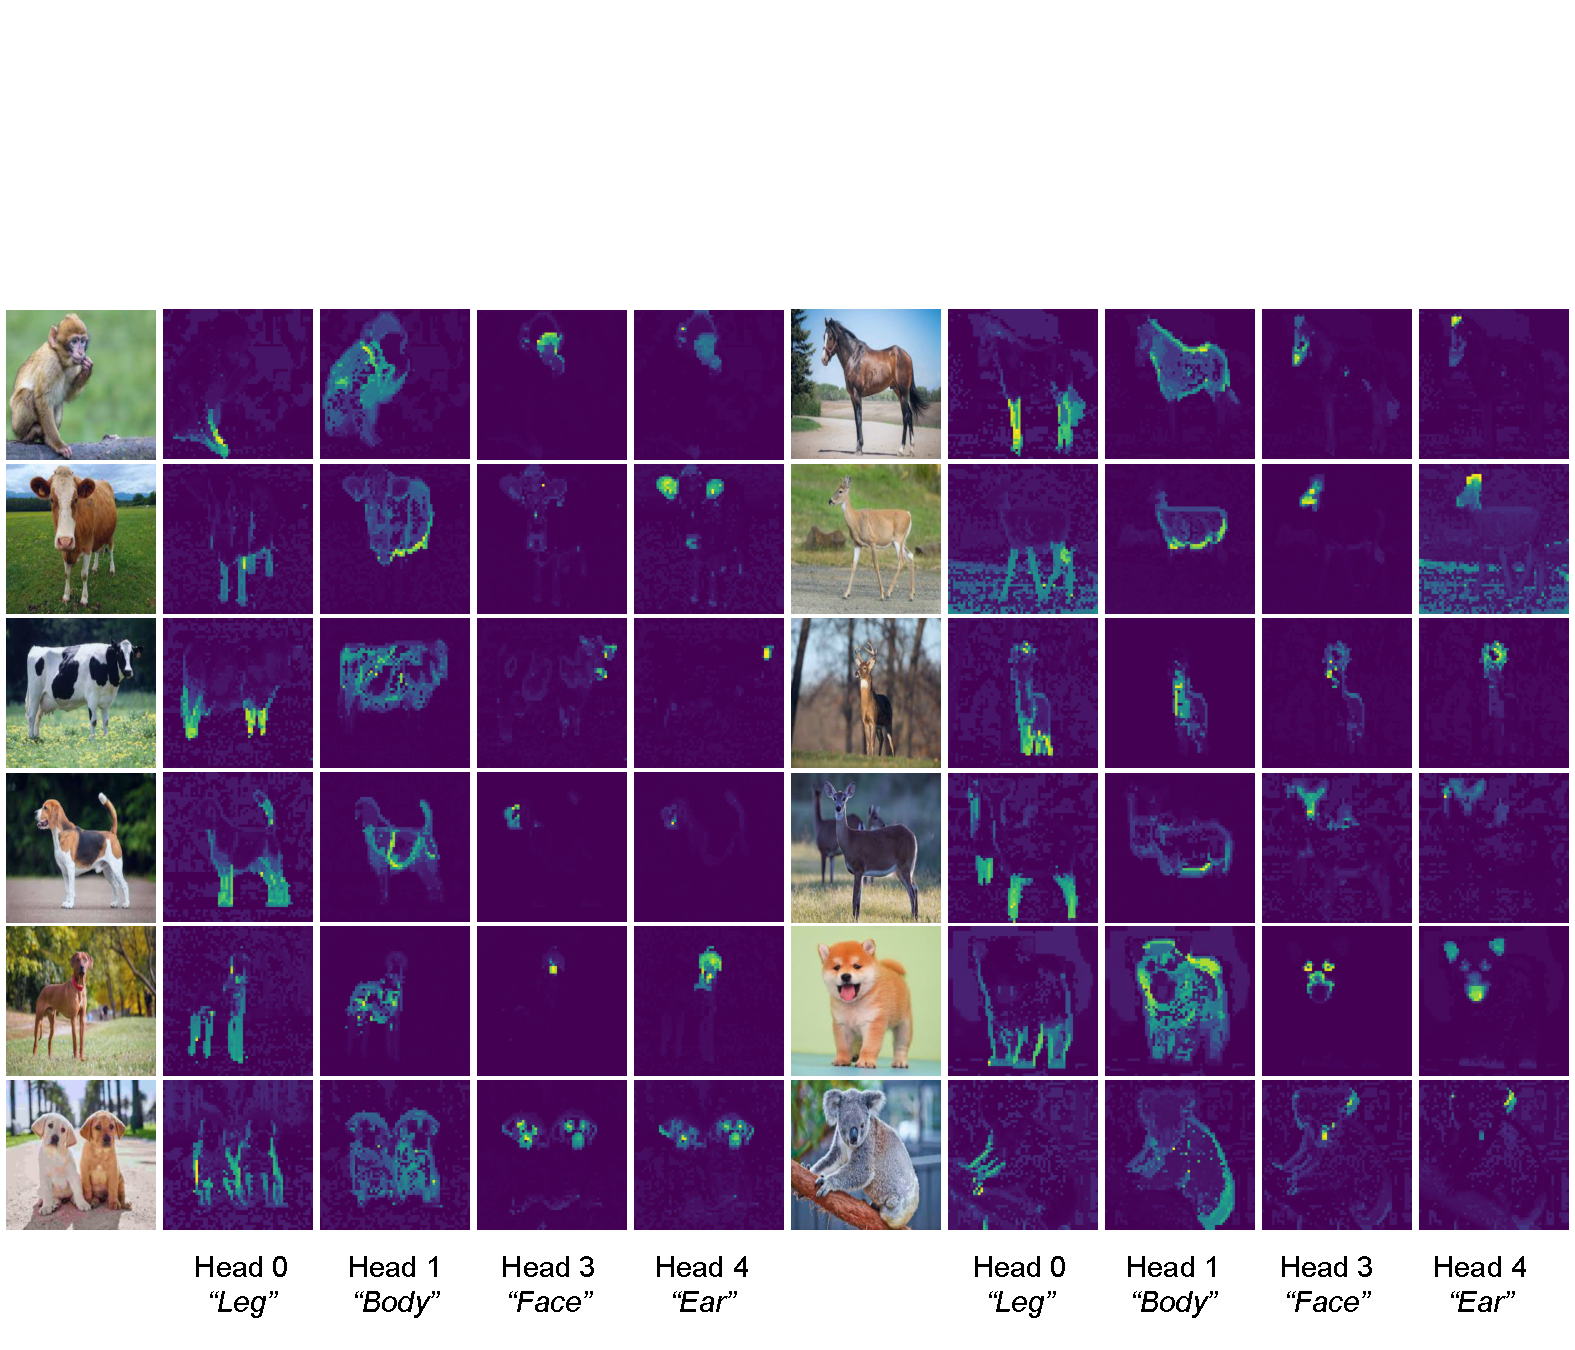
\includegraphics[width=0.8\textwidth]{\toplevelprefix/chapters/chapter7/figs/crate_semantic_heads.pdf}
    \caption{\small\textbf{CRATE中可解释的显著图},图像块大小为\(8\)。当输入具有相似属性的图像时(这些图像可能但不一定来自同一类别),最后一层中不同注意力头对应的显著图分别突显了特定的属性。可以观察到,平均显著图(图中未包含)会突显图像中所有相关的对象,这表明模型利用了输入图像的所有细粒度细节进行分类。据作者所知,这是\textit{第一个}实现此功能的机器学习系统,更不用说它是在没有任何分割数据训练的情况下自动完成的。}
    \label{fig:crate_semantic_heads}
\end{figure}

\begin{table}
    \centering
    \begin{tabular}{@{}lcccccccc@{}}
    \toprule
     &  \multicolumn{3}{c}{检测 (\(\uparrow\))} &  \multicolumn{3}{c}{分割 (\(\uparrow\))} \\ 
    模型 & AP$_{50}$ & AP$_{75}$ & AP & AP$_{50}$ & AP$_{75}$ & AP  \\ 
    \midrule
    CRATE-S/8 & \textbf{2.9} & \textbf{1.0} & 1.1 & 1.8 & \textbf{0.7} & 0.8 \\
    CRATE-B/8 & \textbf{2.9} & \textbf{1.0} & \textbf{1.3} & \textbf{2.2} & \textbf{0.7} & \textbf{1.0} \\
    ViT-S/8 & 0.1& 0.1 & 0.0 & 0.0 & 0.0 & 0.0 \\
    ViT-B/8 & 0.8 & 0.2 & 0.4 & 0.7 & 0.5 & 0.4 \\
    \bottomrule
    \end{tabular}
    \caption{\small \textbf{在COCO {val2017}~\citep{lin2014microsoft}上通过MaskCut进行的目标检测和细粒度分割}。此处所有模型均使用大小为\(8\)的图像块进行训练,而非\(16\)。当两者都使用监督分类进行训练时,CRATE在检测和分割指标上均决定性地优于ViT。}
    \label{tab:crate_detection_segmentation}
\end{table}


\paragraph{实验结果。} 

\Cref{tab:crate_classification_linear_probing}表明,在相似参数数量下,CRATE模型与流行的视觉Transformer(ViT)架构相比,至少在其特征对于不同类别的线性可分性方面,达到了持平或有所改进的性能。在注意力图的保真度方面,\Cref{fig:crate_semantic_heads}展示了一个真正非凡的结果:无需在任何分割或目标检测数据上进行训练,显著图\textit{不仅}有效地捕捉了输入图像的所有相关部分,而且它们还能\textit{自我组织},使得每个显著图都对应于一个离散的概念集,甚至跨越了不同的样本和类别!据作者所知,这是第一个实现此功能的系统,而且它除了图像分类数据外,无需使用任何额外数据即可做到这一点。\Cref{tab:crate_detection_segmentation}从数量上证实了这些定性见解,显示出与在相同监督分类设置下训练的ViT相比有显著的改进。

\section{因果语言建模}\label{sec:clm_text}

我们现在研究\textit{因果语言建模},这是一种训练大型语言模型(LLM)的方法。这与用于训练GPT-2以及许多其他语言模型等的设置是相同的。

\subsection{数据} \label{sub:clm_text_data}

我们将使用OpenWebText(OWT)~\cite{Gokaslan2019OpenWeb}数据集来研究CRATE在语言任务上的性能。OWT是OpenAI用于训练GPT-2的未发布WebText数据集的一个开源复现版本。OWT中的每个样本都是一个网络文档,通常来源于高质量的网页、博客、文章或在线讨论,并以格式良好的自然语言写成。OpenWebText数据集包含约801万份不同长度的文档,总计约41.70GB的文本。评估时,我们将使用几个数据集,例如WikiText~\cite{merity2016pointer}\footnote{对于WikiText2和WikiText103~\cite{merity2016pointer},它们的测试集是相同的,因此我们将它们合并为一个称为WikiText的数据集。}、LAMBADA~\cite{paperno2016lambadadatasetwordprediction}\footnote{为了获得LAMBADA数据集的准确率,我们使用贪婪解码。}和PTB~\cite{marcus-etal-1993-building}。与其他数据集相比,PTB和OWT通常更容易。PTB侧重于较简单的新闻文本,是传统语言建模的理想选择;而OWT则内容多样且非正式,涵盖了各种主题,但在语言结构或长程依赖方面的复杂性较低。WikiText具有正式的结构和领域特定的内容,比OWT需要更复杂的理解,但仍在可控范围内。LAMBADA是最具挑战性的,因为它涉及长程依赖,要求模型掌握更广泛的上下文信息才能准确地完成句子。

在更形式化的层面上,我们的数据\(\vX\)是文本,即字符组成的字符串;我们令\(\cT\)为所有字符串的集合。

\subsection{任务与目标} \label{sub:clm_text_objective}

对于因果语言建模预训练,其思想是我们要\textit{训练模型以输出类似人类的文本}。迄今为止,最流行的方法是使用一个两阶段的训练过程:\footnote{现代语言模型的训练包含几个额外的训练步骤,这些步骤需要不同的数据分布和算法方法。然而,仅仅训练一个模型来模仿人类写作,只需要这里介绍的几个步骤。}
\begin{itemize}
    \item \textit{首先},我们希望\textit{学习}一种将文档最优地编码为一系列基本(“构建块”)字符串的方法,这些字符串被称为\textit{词元}(token)。这个过程称为\textit{分词}(tokenization),我们构建一个\textit{分词器}(tokenizer)。
    \item \textit{其次},我们希望\textit{学习}一种\textit{在给定所有先前词元的条件下预测下一个词元分布}的方法。这个过程称为\textit{下一词元预测},我们构建一个\textit{语言模型}。
\end{itemize}
这个过程实际上可以追溯到马尔可夫,他首先注意到在适当的分词下,自然语言可以用其同名的马尔可夫链结构来建模\citep{markov2006example};之后香农提出了完全相同的语言建模设置,使用字符级分词器(即每个字符是一个词元)和所谓的“\(n\)-gram”模型(即一个显式的查找表,根据训练数据计算得出,用于表示在给定前\(n\)个词元的情况下一个词元的分布)来代替语言模型\citep{Shannon-1948}。\footnote{最近一项研究\citep{liu2024infini}对\(n\)-gram模型进行了扩展,结果表明对于较大的\(n\),它们能够相当好地对文本进行建模,但存储这样一个查找表所需的内存量级为\(V^{n}\),因此是完全不可行的。}

\subsubsection{训练分词器}

构建分词器,相当于构建一个词汇表\(\cV\),它是一个词元的集合,其大小\(V\)是预先指定的。一种流行的算法是字节对编码(Byte Pair Encoding, BPE),可以描述如下:
\begin{itemize}
    \item 从训练数据中所有唯一字符及其频率的列表开始。确保这些字符的数量少于\(V\),并将每个字符作为一个单独的字符串(“词元”)连同其频率添加到词汇表中。
    \item 直到词汇表中有\(V\)个词元为止:
    \begin{itemize}
        \item 通过取两个最频繁的现有词元并将它们合并来构建一个新的词元。
        \item 计算这个新词元在数据集中的频率。
        \item 将其(连同其频率)添加到词汇表中。
    \end{itemize} 
    \item 此时,频率信息不再需要,可以丢弃。
\end{itemize}
BPE的整个过程如图\Cref{fig:BPE}所示。请注意,这个过程是经典信息论中用于\textit{学习字节流数据(如文本)的无损编码}的压缩过程的一种变体,因此,可以将其解释为寻找数据的最优无损压缩。需要注意的是,这是可行的,因为(与图像不同)这里的数据是根本上离散且无噪声的。
\begin{figure}
    \centering
    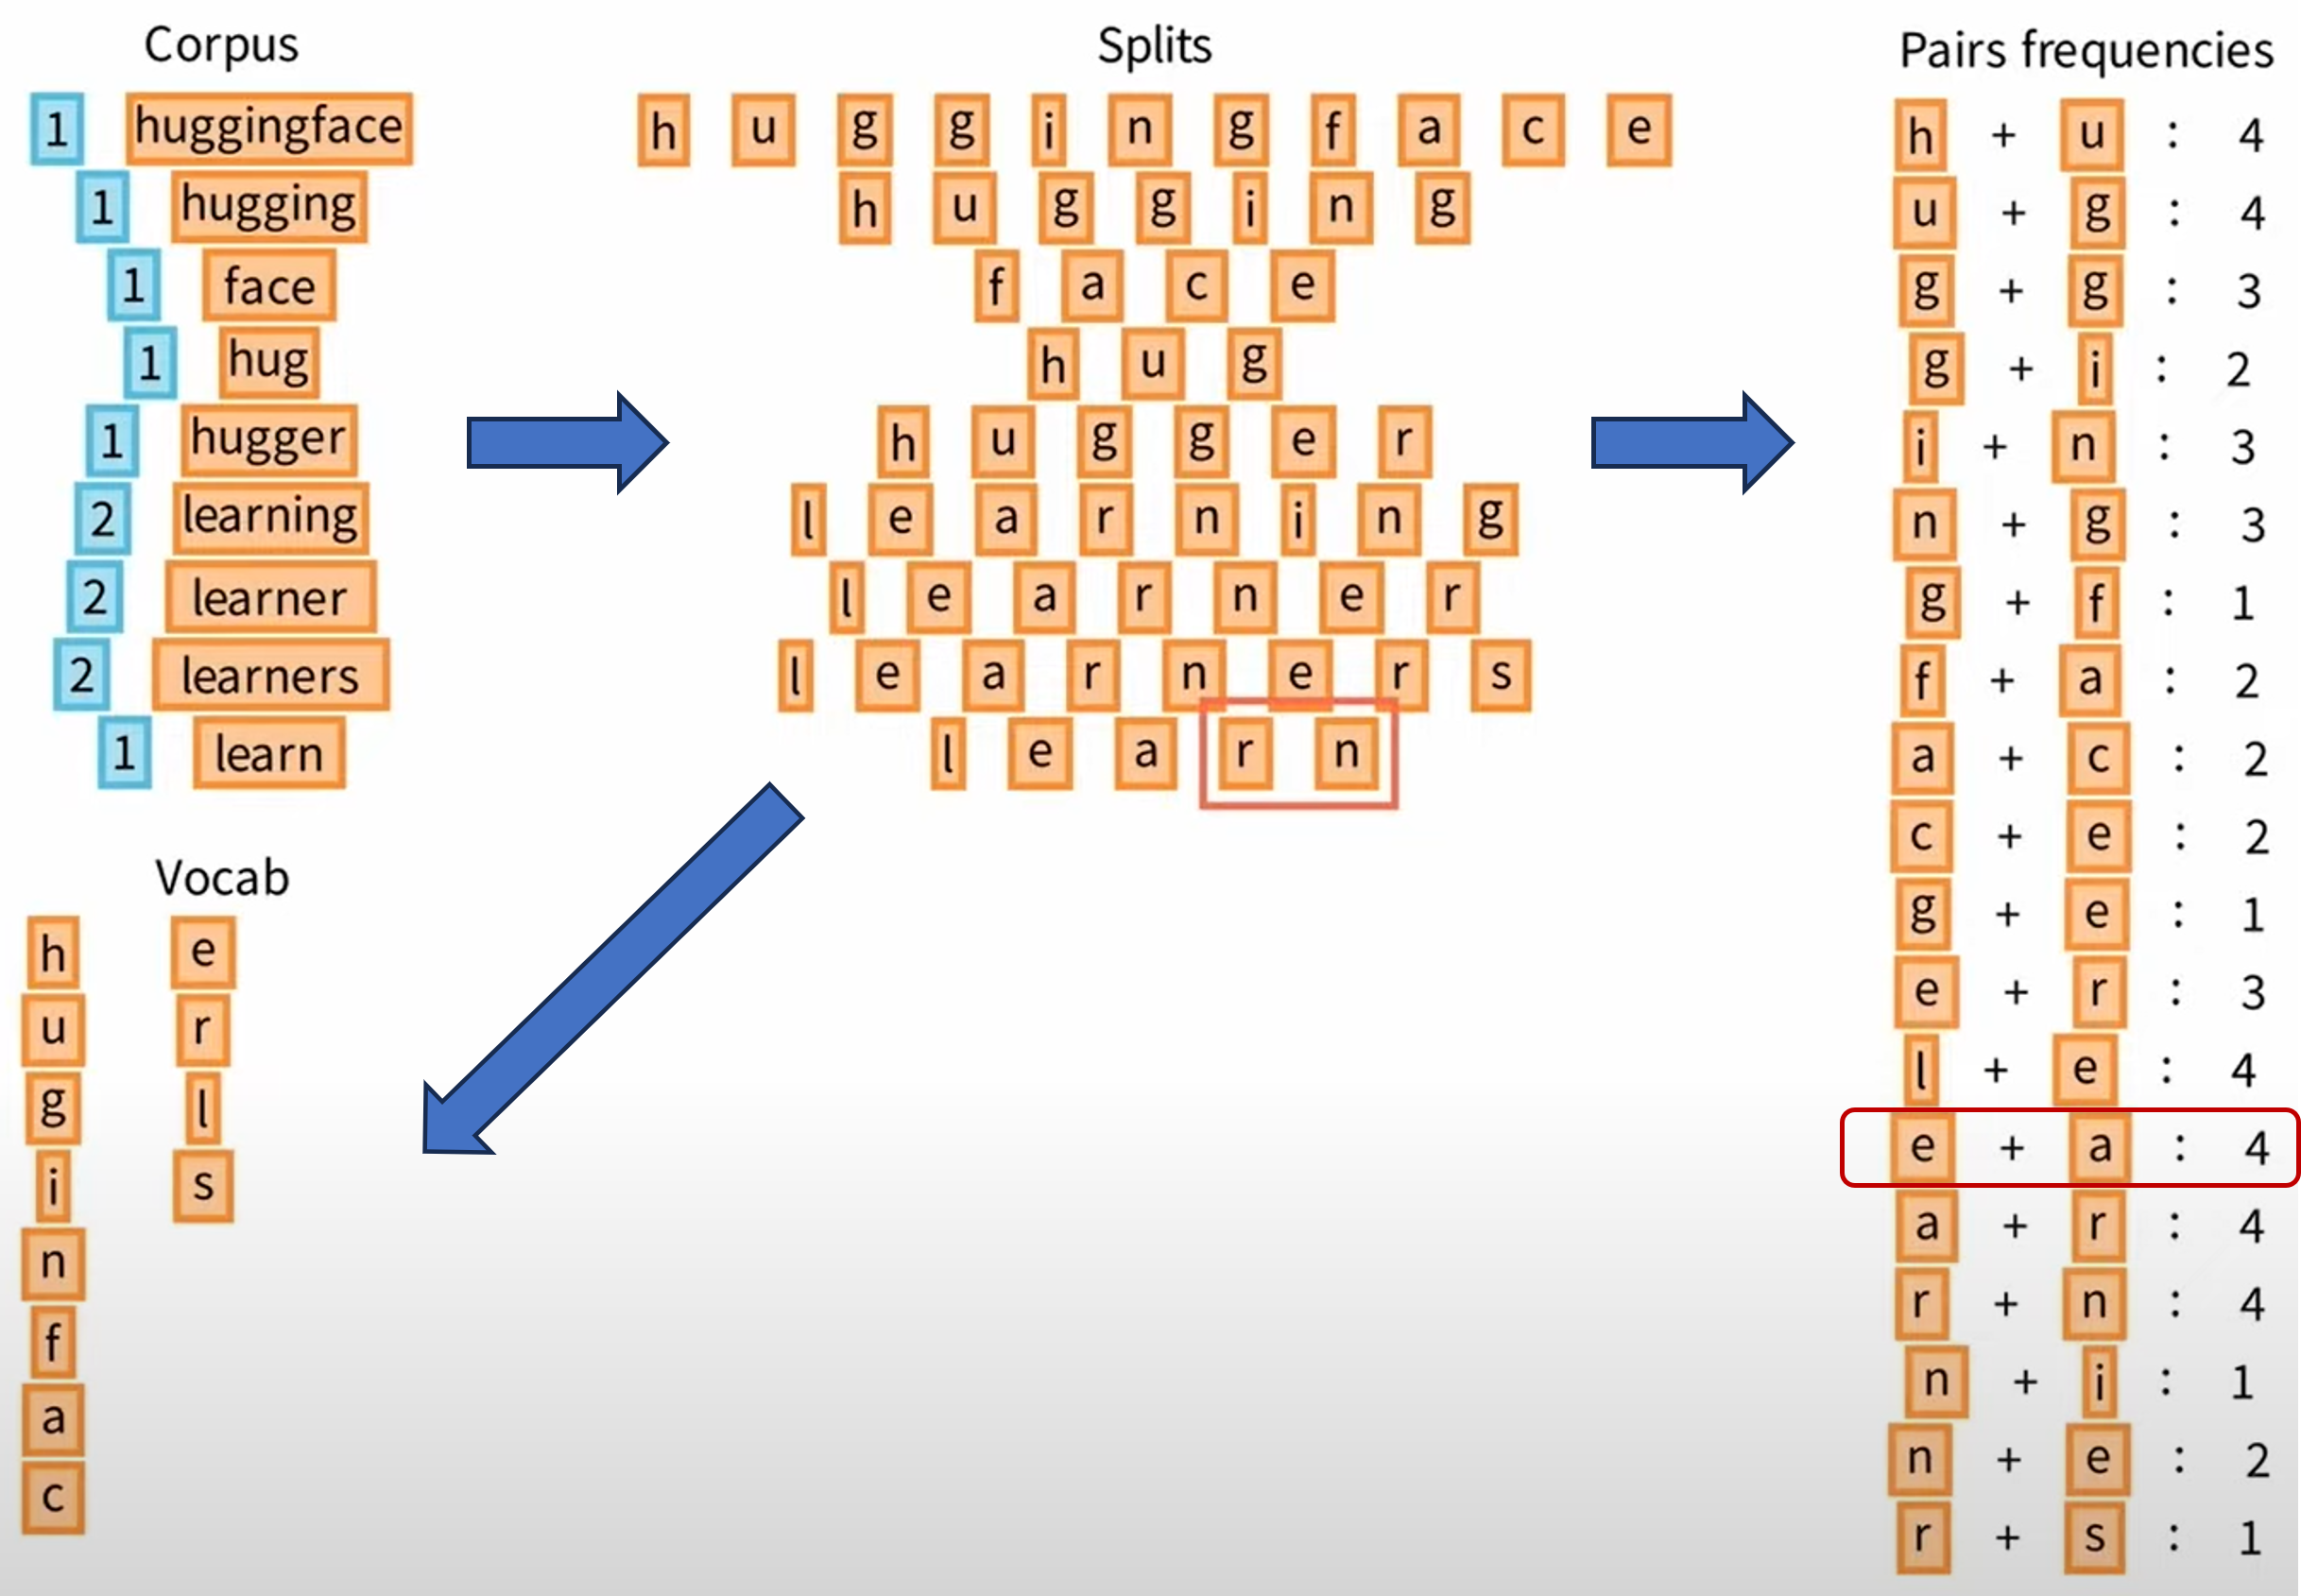
\includegraphics[width=0.45\textwidth]{\toplevelprefix/chapters/chapter7/figs/BPE1.png}\hspace{0.6in} 
    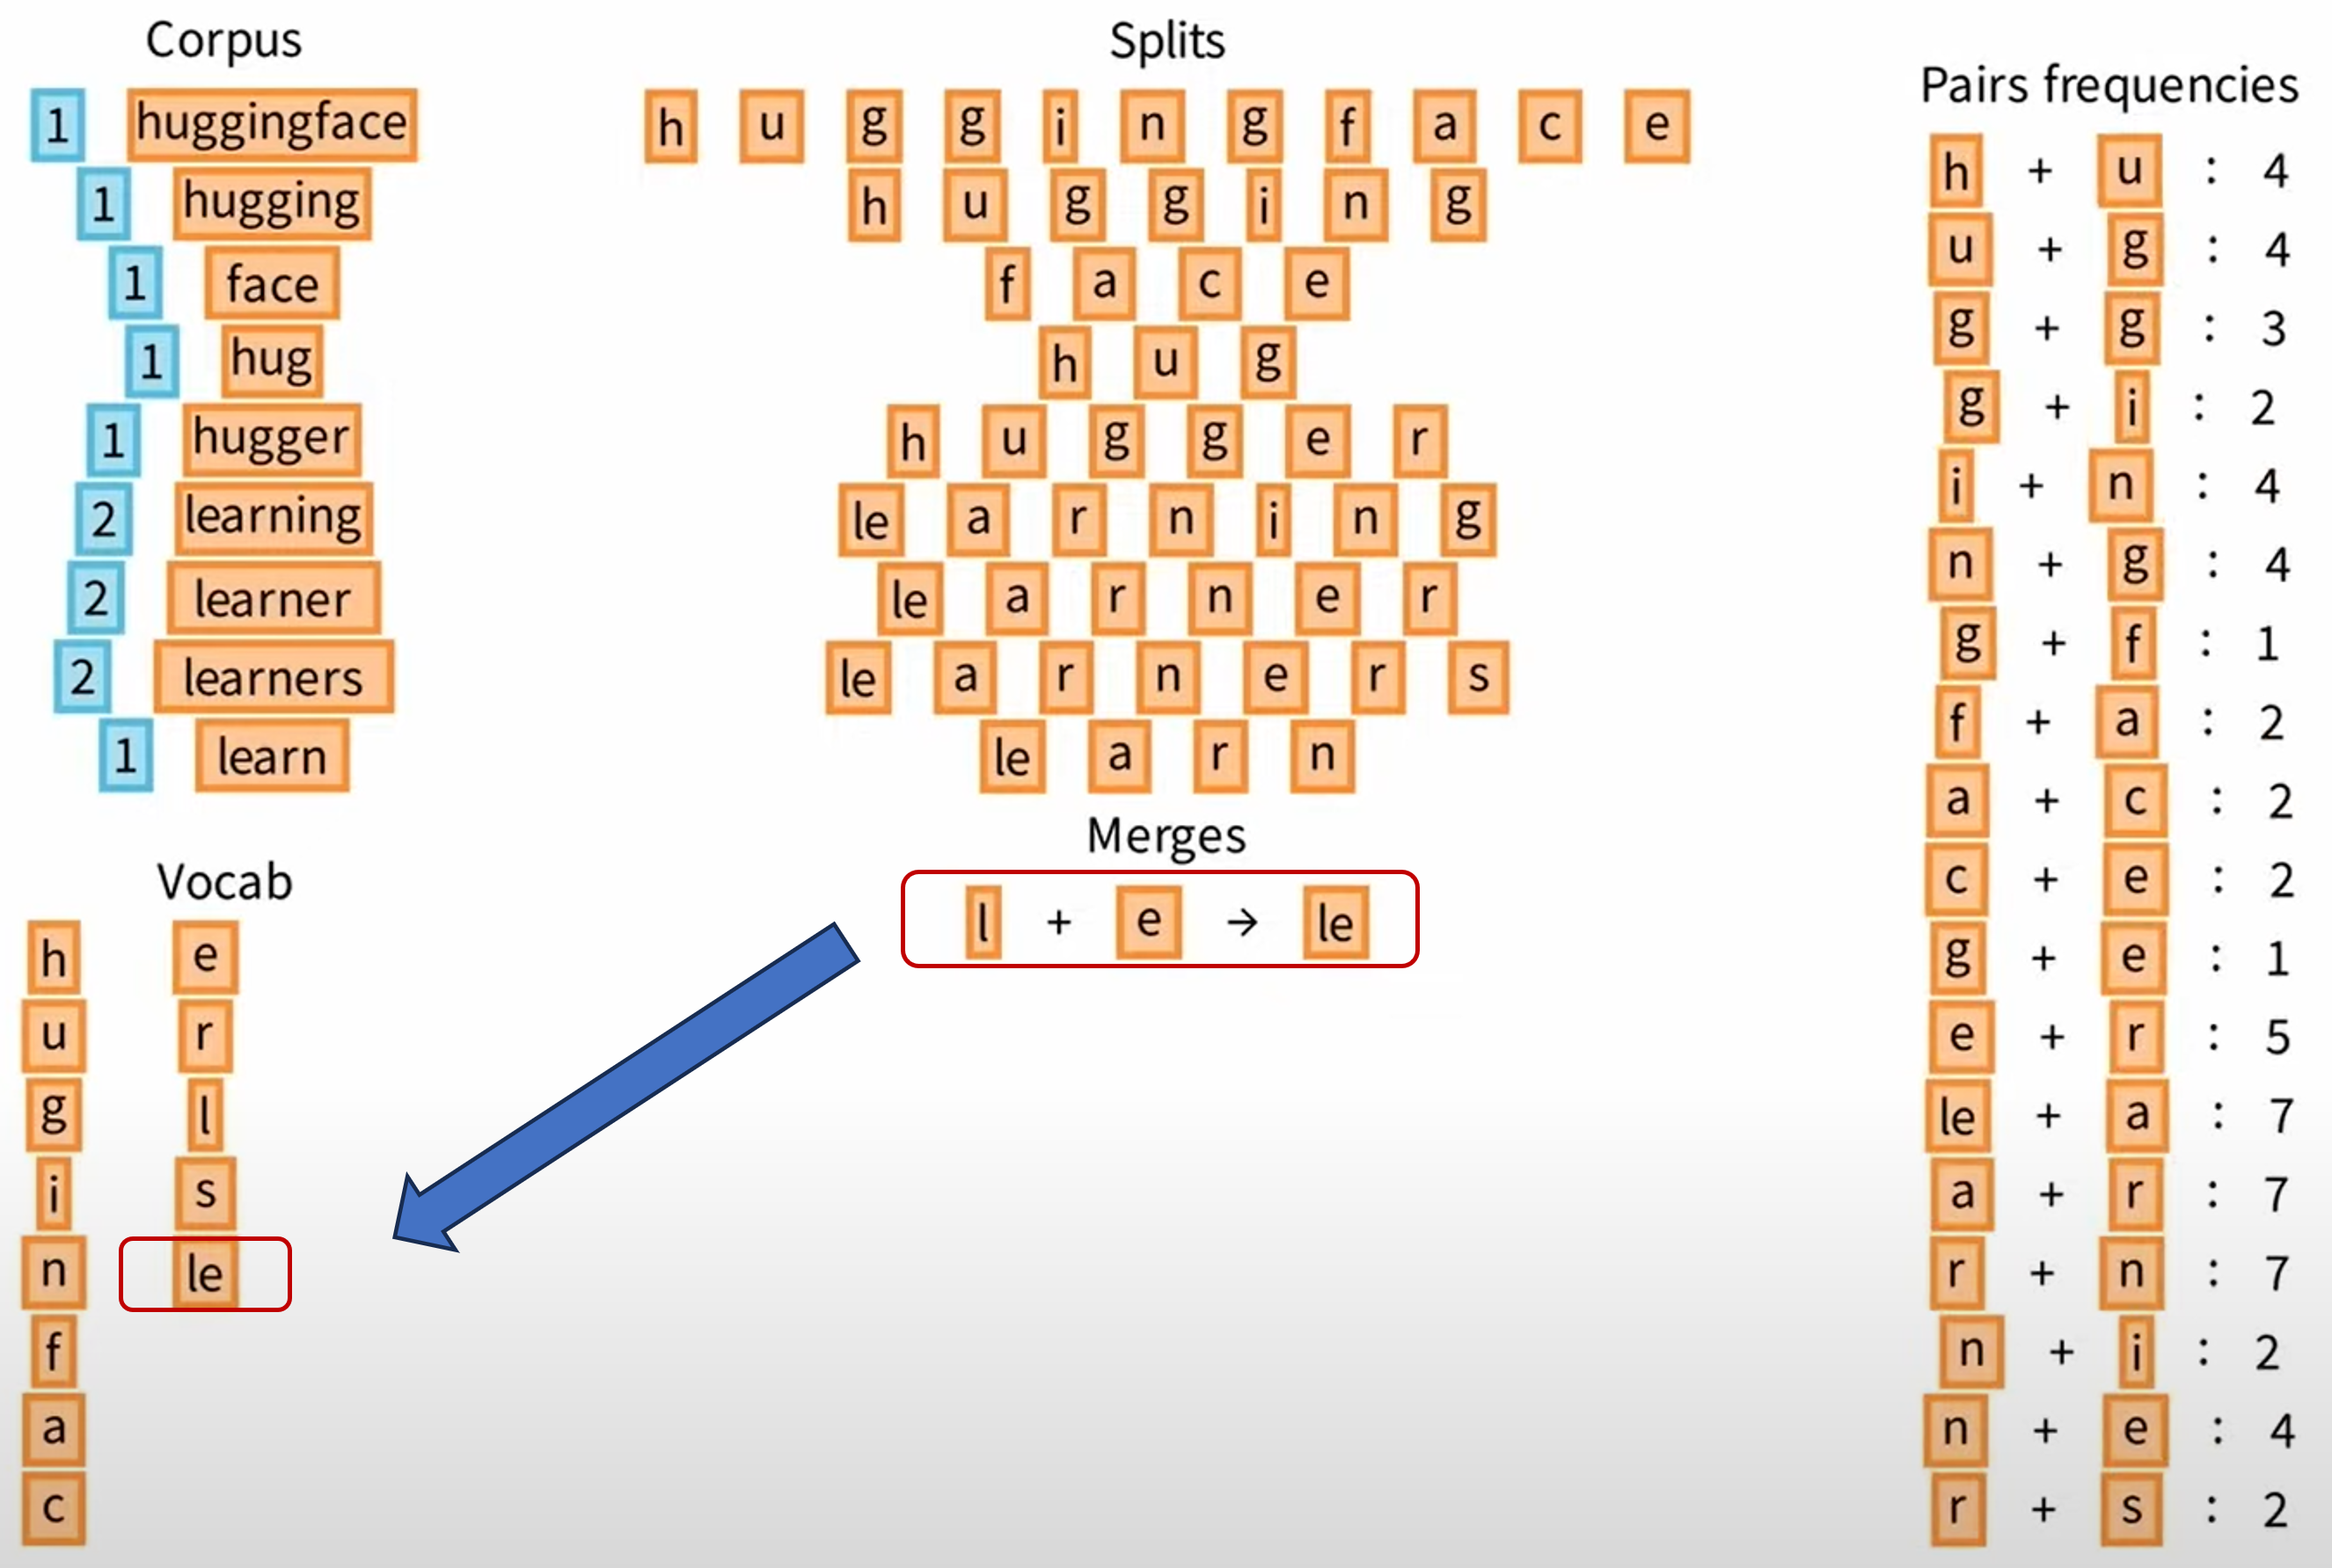
\includegraphics[width=0.45\textwidth]{\toplevelprefix/chapters/chapter7/figs/BPE2.png} 
    \caption{\small {\bf 使用BPE对文本数据进行分词的过程。}(图片来源:\url{https://huggingface.co/learn/nlp-course/chapter6/5})。(左)我们首先分析给定的文本语料库,并构建一个由单个字符(对于字节级BPE,则是字节)组成的初始词汇表。然后,我们计算语料库中相邻字符对的频率。这包括扫描整个文本并统计每个双字符序列(二元组)出现的次数。(右)计算完相邻字符对的频率后,我们找出语料库中最频繁的对。然后将该对合并成一个新的子词单元,并作为一个单独的词元添加到词汇表中。这个过程会迭代重复,直到达到预定义的词汇表大小。 }
    \label{fig:BPE}
\end{figure}
构建好这样的词汇表后,分词器就可以将文档分解为词元(即对其进行“分词”)。BPE使用与训练时类似的过程来对数据进行分词:
\begin{itemize}
    \item 将文档分割成一个由单字符词元组成的长列表。也就是说,如果文档是“Hello”,那么初始列表就是`H', `e', `l', `l', `o'。
    \item 只要任意两个相邻的词元可以连接起来,并且它们的连接结果是另一个词元,我们就执行这个操作,即用合并后的词元替换这对词元。例如,如果`He'是词汇表中的一个词元,那么`H', `e', `l', `l', `o'就会变成`He', `l', `l', `o'。
    \item 重复上述过程,直到无法再进行合并。此时,文档就被分割成了最终的词元列表(序列)。
\end{itemize}

在分词过程中,有许多基于实践和效率的考虑因素。例如,如果朴素地实现,上述算法远非\textit{最优}。我们不详细讨论这个主题;网上有很多资源可以学习更多,例如\href{https://huggingface.co/learn/nlp-course/en/chapter6/5}{HuggingFace教程}。

例如,每个词元都有一个对应的\textit{索引},即它在词汇表(毕竟只是一个长度为\(V\)的列表)中的索引。因此,大多数分词器的输出是一个索引列表,可看作是\([V]^{*}\)中的一个元素。请记住,如上所示,它们对应于原始文档的子字符串。

一旦学习了分词器,任何语言模型都可以将其作为黑盒使用。例如,许多模型都使用基于\texttt{tiktoken}库的相同(基于OpenAI的)分词器。在本节的其余部分,我们将对所有内容使用这样一个固定的、预先构建的分词器,因此将每个文本文档\(\vX \in \cT\)与其在\([V]^{*}\)中的分词版本等同起来。因此,我们不妨将文本空间\(\cT\)视为与词元序列空间\([V]^{*}\)\textit{相等}(并且不会丢失任何本质信息)。

\subsubsection{训练语言模型}

一旦我们将每个文档表示为词元序列\(\vX \in [V]^{N} \subseteq [V]^{*} = \cT\),我们希望执行下一词元预测。也就是说,给定一个\textit{上下文}\(\vX_{:n} \in [V]^{n}\)(即文档中的前\(n\)个词元\(\vx_{1}, \dots, \vx_{n} \in [V]\))\footnote{注意这与Python表示法的不一致:这里的表示法\textit{包含}索引\(n\)。},我们希望预测位置\(n + 1\)处的词元\(\vx_{n + 1} \in [V]\)。为此,我们通过\(\vz_{\theta}(\vX_{:n}) := (f_{\theta}^{\ext} \circ f_{\theta})(\vX_{:n}) \in \R^{d}\)计算\(\vX_{:n}\)的聚合特征,并使用一个分类头\(h_{\theta} \colon \R^{d} \to \Delta_{V}\)(实现为线性层、MLP或更复杂一些的结构)将此特征投影到\(V\)维概率单纯形\(\Delta_{V}\)中。这个投影\(\vp_{\theta}(\vX_{:n}) := h_{\theta}(\vz_{\theta}(\vX_{:n}))\)作为下一个词元的估计概率分布。然后,使用记号\(\vone(\vx_{n + 1}) \in \Delta_{V}\)表示在第\(\vx_{n + 1}\)个分量上为\(1\)其余分量为\(0\)的向量,因果语言建模损失为
\begin{equation}\label{eq:clm_loss}
    \min_{\theta}\bc{\cL_{\mathrm{CLM}}(\theta) := \Ex_{\vX}\rs{\frac{1}{N - 1}\sum_{n = 1}^{N - 1}\CE(\vone(\vx_{n + 1}), \vp_{\theta}(\vX_{:n}))}}
\end{equation}
注意这与分类损失(例如图像分类)是多么相似;都是使用交叉熵,并试图将预测的概率向量与真实标签对齐。这两种损失的主要区别在于,在这里,我们是在整个序列上计算损失,其中每个预测都相互关联(不像在独立同分布的分类情况中)。

在语言模型社区中,优化此损失通常被称为“预训练”(与“后训练”以及最近的“中途训练”形成对比,后者是为有用任务修改下一词元预测器的方法论)。

\textit{旁注:}为什么\eqref{eq:clm_loss}的第一项是预测\(\vone(\vx_{2})\),而没有一项是衡量预测第一个词元的损失?这是因为如果我们想预测第一个词元,上下文将是\textit{空序列},因此这个首词元预测将使用一种与适用于其他词元的机制有质的不同的机制。所以实际上这个模型并没有被训练来预测任何文档的\textit{第一个}词元。这样做是可行的,原因在于分词器的一个实现细节:通常,在构建分词器之后,我们会在其词汇表中插入一个\textit{特殊}词元,称为\textit{字符串(或文档)开始}词元,标记为\texttt{<|bos|>}。\footnote{通常有几种用于不同目的的特殊词元。包含特殊词元的现有文本会经过特殊处理。} 然后,在处理每个文档时,我们在文档的词元序列的开头添加\texttt{<|bos|>}词元,使分词序列的长度增加\(1\)。因此,上述因果语言建模目标中就包含了一项,该项试图在仅给定\texttt{<|bos|>}词元作为上下文的情况下预测文档的第一个词元,所以它在概念上是一个正确的损失函数。

\subsection{架构:因果CRATE}

在架构方面,我们使用标准的GPT-2风格的Transformer,用CRATE层替换Transformer层。\footnote{与本书以及许多其他社区的惯例直接相反,自然语言处理(NLP)社区将这种GPT-2风格的Transformer(包括几乎所有当前的LLM)称为“仅解码器”(decoder-only)的Transformer。“仅编码器”(encoder-only)的Transformer具有不同的架构,而“编码器-解码器”(encoder-decoder)的Transformer则将一个“仅编码器”的Transformer与一个“仅解码器”的Transformer连接起来。尽管“仅解码器”的Transformer\textit{也}会计算数据的编码!} 为完整起见,我们在此处详细说明该架构。

\paragraph{嵌入。} 我们首先将词元序列\(\vX \in [V]^{N}\)嵌入到欧几里得空间中。这通常是通过一个\textit{巨大的}\footnote{我们所说的“巨大”,是指这种结构通常占语言模型总大小的很大一部分。}数组\(\vE \in \R^{V \times d}\)将\([V]\)中的每个索引与\(\R^{d}\)中的一个向量关联起来,并直接形成序列\([\vE_{\vx_{1}}, \dots, \vE_{\vx_{N}}] \in \R^{d \times N}\)。完整的嵌入映射\(f_{\theta}^{\emb}\)还应用了位置编码\(\vE^{\pos} \in \R^{d  \times N_{\max}}\),其中\(N_{\max}\)是可能处理的最大词元数,\footnote{现代的位置编码方法已经解决了这个问题,并允许(理论上)无限外推,但这些方法开发起来更复杂,为简单起见,我们在这里只介绍绝对加性位置编码。}从而得到嵌入映射
\begin{equation}
    f_{\theta}^{\emb}(\vX) := [\vE_{\vx_{1}}, \dots, \vE_{\vx_{N}}] + \vE_{:N}^{\pos}
\end{equation}
参数\(\vE\)和\(\vE^{\pos}\)是直接可训练的。由于\(\vE\)非常大(并且梯度更新相对于它非常稀疏,因为每个样本只使用词汇表的一小部分),因此需要使用专门的软件来确保内存更新不会过于繁重。另请注意,我们不像在其他章节中那样使用类别词元;稍后会详细介绍这一点。

\paragraph{主干网络。} 我们使用一个类似CRATE并采用因果掩码的主干网络来处理嵌入。为了说明因果掩码的动机,考虑\eqref{eq:clm_loss}中定义的因果语言建模损失\(\cL_{\mathrm{CLM}}\)。最朴素的实现需要我们计算\(N\)次前向传播才能进行一次反向传播。显然这是极其低效的,因为\(N\)通常可能达到数千。为了有效地扩展使用此损失的训练,我们施加一个\textit{因果}约束,即
\begin{equation}\label{eq:causal_backbone_def}
    \vZ_{\theta}(\vX_{:n}) = \vZ_{\theta}(\vX)_{:n}
\end{equation}
也就是说,无论\(n\)和\(N\)取何正值(\(N \geq n\)),词元特征\(\vZ_{\theta}(\vX_{:n}) \in \R^{d \times n}\)的\(n\)列应与词元特征\(\vZ_{\theta}(\vX) \in \R^{d \times N}\)的前\(n\)列相同。实际上,这意味着我们可以对整个序列\textit{一次性}应用主干网络来计算\(\vZ_{\theta}(\vX)\),然后随着\(n\)增长到序列长度\(N\),对每个递增的子集\(\vZ_{\theta}(\vX_{:n}) = \vZ_{\theta}(\vX)_{:n}\)应用\(f_{\theta}^{\ext}\)。然后我们可以用所有这些来计算损失。

既然我们想要一个因果架构的主干网络,我们该如何实现呢?由于每个Transformer层内部的MLP和层归一化都单独作用于每个词元,因此对于因果性而言,唯一重要的是注意力块(在CRATE中是\(\MSSA\))。为了使\(\MSSA\)具有因果性,我们定义\(\mathrm{CausalMSSA}\)块为
\begin{align}
    &\operatorname{CausalMSSA}_{\theta}^{\ell}(\vZ) := \vU_{\out}^{\ell}\mat{\operatorname{CausalSA}([\vU^{1, \ell}]^{\top}\vZ, [\vU^{1, \ell}]^{\top}\vZ, [\vU^{1, \ell}]^{\top}\vZ) \\ \vdots \\ \operatorname{CausalSA}([\vU^{K, \ell}]^{\top}\vZ, [\vU^{K, \ell}]^{\top}\vZ, [\vU^{1, \ell}]^{\top}\vZ)} + \vb_{\out}^{\ell}\vone_{N}^{\top} \\ 
    \text{其中} \quad & \operatorname{CausalSA}(\vQ, \vK, \vV) := \vV\softmax\rp{\frac{\operatorname{CausalMask}(\vK^{\top}\vQ)}{\sqrt{p}}} \\ 
    \text{其中} \quad & \operatorname{CausalMask}(\vM)_{ij} = \casework{M_{ij}, & \text{若}\ i \geq j, \\ -\infty, & \text{若}\ i < j}.
\end{align}
在这里,从业者称因果掩码\textit{允许未来的词元\(i\)关注过去的词元\(j\),但反之则不然}。为了理解原因,让我们写出\(\operatorname{CausalSA}(\vQ, \vK, \vV)\)的第\(t\)列的表达式:
\begin{equation}
    \operatorname{CausalSA}(\vQ, \vK, \vV)_{t} = \sum_{i = 1}^{t}\vV_{i}\softmax\rp{[\vK_{:t}]^{\top}\vQ_{t}}_{i}
\end{equation}
(这里非冒号下标表示列)。这个第\(t\)个词元的表达式没有使用任何超出索引\(t\)的词元信息。因此,\(\operatorname{CausalSA}\),进而\(\operatorname{CausalMSSA}\),乃至整个因果CRATE主干网络,根据\eqref{eq:causal_backbone_def}中的定义都是因果的,从而我们获得了所承诺的可观效率提升。

\paragraph{特征提取器。} 我们使用一个后处理步骤\(f_{\theta}^{\ext}\),它提取\textit{最后一个已知词元的特征向量}来预测下一个词元。理论上,这意味着每个词元\(\vZ_{\theta}(\vX)_{n}\)应包含关于所有在索引\(n\)之前或之上的词元(即\(\vx_{1}, \dots, \vx_{n}\))的丰富信息,因为所有这些信息都应该可用于预测索引\(n + 1\)处的下一个词元。在实践中,每个预测任务实际上只需要这些词元中的少数几个。无论如何,\(f_{\theta}^{\ext}\)的方程为
\begin{equation}
    f_{\theta}^{\ext}(\vZ_{\theta}(\vX_{:n})) := (\vZ_{\theta}(\vX))_{n}
\end{equation}
其中(再次强调)非冒号下标是列。在这种情况下,如所承诺的,我们只是直接提取序列中最后一个词元的特征向量。

\paragraph{任务特定头。} 对于我们的分类头\(h_{\theta}\),GPT-2架构使用一个简单的线性层和一个softmax来获得所需的概率向量:
\begin{equation}
    h_{\theta}(\vz) := \softmax(\vW^{\out}\vz + \vb^{\out}),
\end{equation}
其中\(\vW^{\out} \in \R^{V \times d}, \vb^{\out} \in \R^{V}\)。一些其他更现代的架构使用小型的MLP和层归一化,但思想非常相似。请注意,这个线性层也占用大量内存(因为\(V\)非常大),并成为训练中的瓶颈;已经有大量的努力试图规避它。

所有这些架构选择意味着因果训练相对于非因果训练效率极高:
\begin{itemize}
    \item 我们只需要通过主干网络进行\textit{一次前向传播}即可计算整个序列的损失。
    \item 特征提取基本上是\textit{免费的}。
    \item 所有词元都可以\textit{并行地}通过任务特定头。
\end{itemize}

\subsection{优化策略}

我们使用端到端随机优化来训练我们的语言模型。一个尚存的问题是,在实践中,一个批次中的不同文档具有不同的长度(就每个序列所需的词元数量而言),但在撰写本书时,主流的深度学习框架大都只允许“矩形”张量,这无法适应这种行为。为了解决这个问题,我们只需为批次中所有较短的样本插入一个特殊的填充词元\texttt{<|pad|>}, 这样我们就可以使用矩形张量来批量处理所有内容。在每个时间步\(k\),我们:
\begin{itemize}
    \item 子采样\(B\)个不同的分词后文档\(\{\vX_{b}^{(k)}\}_{b = 1}^{B} \subseteq \cT = [V]^{*}\),每个文档的长度为\(N_{b}^{(k)}\)。
    \item 计算\(N_{\max}^{(k)} := \max_{b \in [B]}N_{b}^{(k)}\)并使用一个特殊的填充词元将每个\(\vX_{b}^{(k)}\)填充到长度\(N_{\max}^{(k)}\)。
    \item 计算特征\(\vZ_{\theta}(\vX_{b}^{(k)})\)。
    \item 计算预测分布\(\vp_{\theta}(\vX_{b, :n}^{(k)}) := (h_{\theta} \circ f_{\theta}^{\ext})(\vZ_{\theta}(\vX_{b}^{(k)})_{:n})\)。
    \item 构建代理随机损失
    \begin{equation}
        \hat{\cL}_{\mathrm{CLM}}^{(k)}(\theta) := \frac{1}{B(N_{\max}^{(k)} - 1)}\sum_{b = 1}^{B}\sum_{n = 1}^{N_{\max}^{(k)}-1}\CE(\vone(\vx_{b, n + 1}^{(k)}), \vp_{\theta}(\vX_{b, :n}^{(k)}))).
    \end{equation}
    \item 对\(\theta\)执行一步优化算法,得到以下迭代:
    \begin{equation}
        \theta^{(k + 1)} := \textsc{OptUpdate}^{(k)}(\theta^{(k)}; \nabla_{\theta}\hat{\cL}_{\mathrm{CLM}}^{(k)}).
    \end{equation}
\end{itemize}

\subsection{评估方法} \label{sub:clm_text_evals}

有几种方法可以评估一个训练好的Transformer语言模型。
\begin{itemize}
    \item 在一个任意文本的留出数据集上,我们可以评估其上的\(\cL_{\mathrm{CLM}}\);损失越低越好,因为这意味着模型的采样能产生更好的性能。
    \item 在一个多项选择题数据集上,对于每个问题,我们可以将其作为上下文,并检查生成正确答案的估计概率。
    \item 我们还可以测试\textit{文本生成}能力。也就是说,我们可以根据上下文从模型的下一个词元概率分布中重复采样。每次采样我们都会生成一个新的词元,我们将其打印出来并添加到上下文中。这使我们能够从LLM中采样,并以我们喜欢的任何方式评判生成的样本。\footnote{每次都必须为每个词元重新运行模型可能会变得极其昂贵。通过巧妙地存储语言模型的不同内部特征(例如所谓的\textit{\(K\)-\(V\)缓存}),结合架构的因果性,可以显著降低采样的成本。}
\end{itemize}
在本节中,我们只进行第一种评估。

\subsection{实验设置与结果}

由于我们的因果CRATE架构直接建立在GPT-2之上,我们将NanoGPT仓库\citep{nanogpt}给出的GPT-2的最优设置与应用于CRATE的相同设置进行比较,以实现公平对比。

\paragraph{模型架构。} 我们使用GPT-2分词器,其词汇表大小为\(V = 50257\),包括一个用于\texttt{<|pad|>}的特殊词元。\footnote{此设置中不包括\texttt{<|bos|>}词元,尽管它在现代语言模型中非常常见。} 上下文长度为\(N_{\max} = 1024\)。主干模型遵循GPT2-Base架构\citep{radford2019language},并进行了适当的修改以包含因果CRATE层,我们与GPT2-Small和GPT2-Base进行比较。

\paragraph{数据集与优化。} 为了训练因果CRATE,我们遵循NanoGPT仓库\citep{nanogpt}中的实现。具体来说,我们使用384的批处理大小,并使用Adam优化器~\citep{kingma2014adam}训练600,000步。对于Adam优化器,我们使用$(\beta_1, \beta_2)=(0.9, 0.95)$和0.1的权重衰减。对于学习率调度,我们应用线性预热和余弦衰减,在第$2,000$次迭代时达到峰值$\eta=6\times 10^{-4}$,最小值为$6\times 10^{-5}$。训练和验证损失随迭代次数的变化如\Cref{fig:crate-text-evals}所示。在使用384的批处理大小和600,000次迭代进行训练后,训练/验证损失收敛到大约$3.37$。相比之下,开放的GPT-2实现在OpenWebText上以512的批处理大小和600,000步进行预训练,并收敛到$2.85$的验证损失\citep{nanogpt}。

\begin{figure}
    \centering
    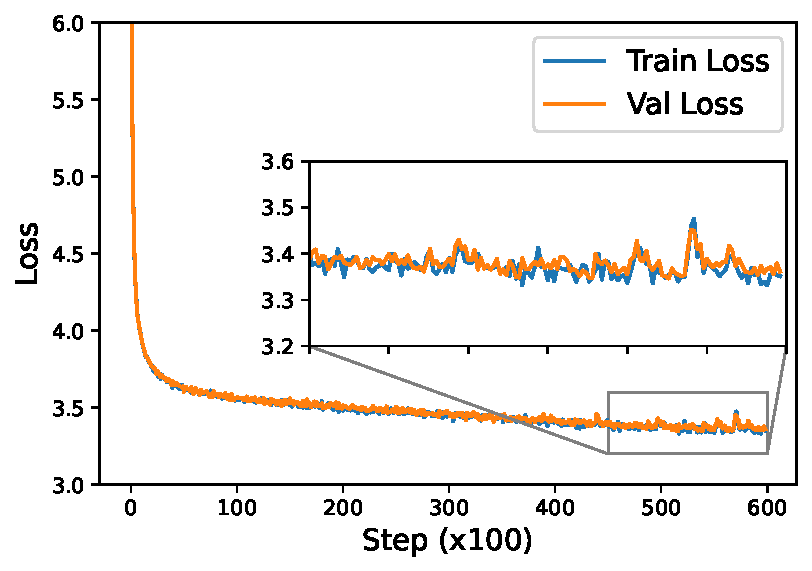
\includegraphics[width=0.5\textwidth]{\toplevelprefix/chapters/chapter7/figs/gpt-loss.pdf}
    \caption{\bf 在OpenWebText数据集上训练的CRATE-GPT-Base的损失曲线。}
    \label{fig:crate-text-evals}
\end{figure}

\paragraph{实验结果。}

\Cref{tab:gpt-eval}表明,与具有相似参数数量和相似架构的GPT-2模型相比,CRATE模型在各种数据集上的因果语言建模损失方面取得了合理的性能。


\begin{table}
\def\arraystretch{1.1}
    \small
    \caption{\small CRATE-GPT2-Base模型以及GPT2-Small、GPT2-Base模型在各数据集测试集上评估的零样本交叉熵损失($\downarrow$越低越好)。
    }
    \centering
    \begin{tabular}{ccccccc}
    \hline
    & \#参数 & \textbf{OWT} & \textbf{LAMBADA} & \textbf{WikiText} & \textbf{PTB} & \textbf{平均} \\
     \hline
     GPT2-Base  & {124M} & 2.85$\downarrow$ & 4.12$\downarrow$ & 3.89$\downarrow$ & 4.63$\downarrow$ & 3.87$\downarrow$ \\
     {GPT2-Small } &  {64M} & {3.04} & {4.49} & {4.31} & {5.15} & {4.25} \\
     Causal-CRATE-Base & {60M} & 3.37 & 4.91 & 4.61 & 5.53 & 4.61 \\
     \hline
    \end{tabular}
    \label{tab:gpt-eval}
\end{table} 


% 为了探索CRATE架构在语言任务上的应用,我们使用以下数据集。对于预训练,我们使用OpenWebText (OWT)~\cite{Gokaslan2019OpenWeb},这是一个开源的、对OpenAI用来训练GPT2的未发布WebText数据集的复现。OWT中的每个样本都是一个网络文档,通常来源于高质量的网页、博客、文章或在线讨论,并展现出格式良好的自然语言。对于零样本评估,我们在WikiText~\cite{merity2016pointer}\footnote{对于WikiText2和WikiText103~\cite{merity2016pointer},测试集是相同的,因此我们将它们合并为一个数据集,称为WikiText。}、LAMBADA~\cite{paperno2016lambadadatasetwordprediction}\footnote{为了在LAMBADA数据集上获得准确率,我们使用贪婪解码。}和PTB~\cite{marcus-etal-1993-building}上评估交叉熵验证损失。在PTB和OWT上训练通常比其他数据集更容易。PTB侧重于更简单的 journalistic 文本,非常适合传统的语言建模,而OWT则多样化且非正式,涵盖了各种主题,但在语言结构或长程依赖方面的复杂性较低。WikiText具有正式的结构和领域特定的内容,比OWT需要更复杂的理解,但仍然是可控的。LAMBADA是最具挑战性的,因为它涉及长程依赖,要求模型掌握更广泛的上下文信息才能准确地完成句子。



% 此外,我们计算LAMBADA上预测句子最后一个词的零样本准确率,以及在儿童图书测试(CBT)~\cite{hill2016goldilocksprinciplereadingchildrens}上的准确率,该任务是从10个可能的选项中为段落中省略的词选择普通名词或命名实体。

% \subsection{任务与目标}

% 对于GPT预训练,我们采用字节对编码(BPE)分词器作为默认分词器,将每个文档转换为词元,词汇表大小为$V=50257$,遵循GPT2的设置\cite{radford2019language}。这里,BPE是一种子词分词算法,它迭代地合并语料库中最频繁的相邻字符对,以创建一个子词词汇表。具体来说,它从一个由单个字节组成的词汇表开始,然后重复地将最常见的对组合成新的子词词元,直到达到预定义的词汇表大小$V=50257$;参见\Cref{fig:BPE}。使用BPE分词器,输入被表示为一个由$N$个词元组成的序列$\bm X = [\bm x_1,\dots,\bm x_{N}] \in \R^{D \times N}$。特别地,由于每个序列可能有不同的长度,我们需要标准化它们的尺寸以确保模型的输入统一。为了解决这个问题,我们应用填充,即用一个特殊的填充词元(通常表示为“[PAD]”或具有特定ID的词元,例如0)来扩展较短的序列,直到它们匹配一个固定的长度。值得注意的是,填充词元在模型计算过程中通过掩码被忽略,确保它们不参与模型的训练。



% 一般来说,CRATE的目标是学习一个映射$f$,该映射将初始词元转换为结构化和紧凑的词元表示,记为$\bm Z$,以促进语言任务。现在,我们介绍关于这个映射$f$的细节。一旦文本被分词为单个词元,GPT2就将每个词元映射到一个稠密向量,该向量由实数值组成。这些向量被称为{\em 词元嵌入},并存储在一个称为嵌入矩阵的查找表中。在GPT2中,嵌入大小通常为768,这意味着每个词元被转换为一个768个浮点数的向量。这些词元嵌入不是固定的,而是在训练过程中学习的。最初,嵌入是随机分配的,但随着训练的进行,它们通过反向传播进行调整,以更好地捕捉词元的语义。在计算出词元嵌入后,GPT2添加位置嵌入以捕捉序列中词元的顺序。位置编码被添加到词元嵌入中,以便为模型提供关于输入序列中每个词元位置的信息。位置编码向量也是学习得到的,并且与词元嵌入具有相同的维度(在GPT2中为768)。形式上,我们将预处理层写为:
% \begin{align*}
%     f^{\rm pre}(\vX) = f^{\rm embed}(\vX) + \vE_{\rm pos}, 
% \end{align*}
% 其中$f^{\rm embed}$是一个嵌入函数,它将输入词元$\vx_i$映射到$\R^d$中的嵌入向量,而$\bm E_{\rm pos}$是在\cite{vaswani2017attention}中定义的正弦位置嵌入。接下来,我们采用CRATE架构(参见\Cref{sub:image_classification_architecture})来构建映射$f$的中间层。这些中间层被设计为迭代地精炼词元表示,逐步从输入序列中捕捉更复杂和更高层次的语义结构。



% GPT-2中的最终输出层采用线性变换的形式,通常被称为{\em 线性头}。该层负责根据模型Transformer层处理过的表示生成最终的输出词元。形式上,最终输出层采用以下形式:
% \begin{align*}
%     f^{\rm head}(\vZ) = \vW^{\rm head}\vZ,
% \end{align*}
% 其中$\vW^{\rm head} \in \R^{V\times d}$是输出权重矩阵。

% GPT的训练目标是下一词预测(因果语言建模),定义为
% \begin{align*}
%     \cL_{\rm GPT}\left(f ,f^{\rm head}\right) = \mathbb{E}_{\vX}\left[ \frac{1}{N - 1}\sum_{i=1}^{N-1} \CE\left(\mathbf{1}(\bm x_{i+1}), \mathrm{softmax}\left\{ (f^{\rm head} \odot f)(\bm X)_i \right\}\right) \right],
% \end{align*}
% 其中$ (f^{\rm head} \odot f)(\bm X)_i \in \R^V$表示模型输出的第$i$个索引(即词汇表中每个潜在词元占据序列$\bm X$中第$i$个索引的对数概率),而$\mathbf{1}(\bm x_{i}) \in \{0,1\}^V$表示词元$\bm x_i$在词汇表中的独热嵌入向量。值得注意的是,模型被训练来使用第$i$个模型输出来预测第$(i+1)$个位置的词元,而不是第$(i+1)$个输出,因为后者会引入循环依赖。这个目标训练模型最大化在序列中每个位置正确预测下一个词元的可能性,同时使用交叉熵损失最小化预测误差。模型以自回归方式运行,这意味着后面位置的预测依赖于前面位置的正确预测。

% \begin{figure}[t]
%     \centering
%     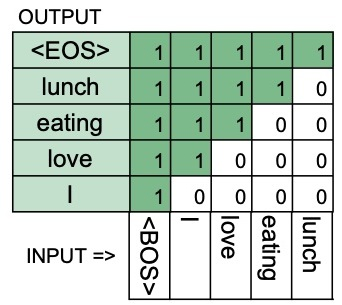
\includegraphics[width=0.3\textwidth]{\toplevelprefix/chapters/chapter7/figs/causal.jpg} 
%     \caption{\small {\bf GPT2中的因果掩码。}(图片来源:\url{https://github.com/sshleifer/blog_v2/blob/master/_notebooks/2020-03-12-bart.ipynb})}.
%     \label{fig:causal}
% \end{figure}

% \subsection{因果CRATE架构}

%     我们在这里使用的CRATE架构与\Cref{sub:image_classification_architecture}中的相似,但进行了一些修改以适应语言任务。遵循\cite{radford2019language}中的设置,我们通过引入一个因果掩码来调整CRATE架构,以与GPT中的下一词预测任务保持一致。在标准的Transformer中,使用因果掩码来防止自回归生成过程中的信息泄漏,方法是确保每个词元只能关注序列中先前和当前的词元;参见\Cref{fig:causal}。这个约束强制执行了一个从左到右的生成过程,这对于语言建模等任务至关重要。数学上,给定一个长度为$T$的序列,GPT2 \cite{radford2019language}中矩阵$\bm A \in \R^{T\times T}$的因果掩码定义如下:
% \begin{align}\label{eq:mask}
%     \mathrm{CausalMask}(\bm A)_{ij} = \begin{cases}
%         A_{ij},\quad \text{若}\ i \ge j,\quad (\text{允许关注过去和当前的词元}) \\
%         -\infty,\quad \text{若}\ i < j. \quad (\text{阻止关注未来的词元})
%     \end{cases}
% \end{align}
% 我们应该指出,因果掩码在自回归设置中至关重要,因为GPT风格的模型是顺序生成文本的——每个词元都仅基于先前看到的词元进行预测。接下来,带有因果掩码的CRATE架构中的MSSA算子可以表示为:
% \begin{align*}
% \mathrm{CausalMask}\MSSA_{\theta}^{\ell}(\vZ) = \sum_{k=1}^K \bm U_k\bm U_k^T \bm Z\mathrm{softmax}\left( \mathrm{CausalMask} \left( \bm Z^{T}\bm U_k \bm U_k^T\bm Z\right) \right),    
% \end{align*}
% 其中$\bm Z$是输出。通过整合这种因果注意力机制,CRATE架构能够在语言建模任务中实现高效计算。它确保模型以顺序方式处理词元,每个词元只关注先前的词元和自身的表示。这种机制降低了允许未来词元影响当前预测所带来的计算复杂性,使模型更高效,更适合于下一词预测等任务。将这个算子代入\eqref{eq:CARTE updates}中的更新规则,就得到了为语言任务优化的最终CRATE架构,既保留了效率,又保证了自回归生成所需的准确性。



% \subsection{优化方法}

% 对于GPT预训练,我们主要遵循nano GPT仓库\cite{nanogpt}中的实现。具体来说,我们使用384的批处理大小,并使用Adam优化器~\citep{kingma2014adam}训练600,000步。对于Adam优化器,我们使用$(\beta_1, \beta_2)=(0.9, 0.95)$和0.1的权重衰减。对于学习率调度器,我们应用线性预热和余弦衰减,在第$2,000$次迭代时达到峰值$\eta=6\times 10^{-4}$,最小值为$6\times 10^{-5}$。训练和验证损失随迭代次数的变化如图~\ref{fig:crate-text-evals}所示。在使用384的批处理大小和600,000次迭代进行训练后,训练/验证损失收敛到大约$3.37$。相比之下,开放的GPT-2实现在OpenWebText上以512的批处理大小和600,000步进行预训练,并收敛到$2.85$的验证损失\citep{nanogpt}。

% \subsection{评估与结果}

% 我们通过在不同数据集上测量零样本交叉熵损失来评估CRATE-GPT模型。数学上,序列$\bm X = [\bm x_1,\dots,\bm x_N]$的零样本交叉熵损失计算如下:
% \begin{align*}
%     \mathcal{L}_{\rm zero-shot} = -\sum_{i=2}^N \log \left(\mathrm{softmax}\left\{ (f^{\rm head} \odot f)(\bm X)_i \right\}\right),
% \end{align*}
% 其中$\mathrm{softmax}\left\{ (f^{\rm head} \odot f)(\bm X)_i \right\}$是模型基于先前词元$\bm x_{1:i-1}$对词元$\bm x_{i}$的预测概率。我们在OpenWebText (OWT)以及\citep{radford2019language}中展示的其他数据集上评估CRATE-GPT-Base。我们与在WebText上预训练的GPT2-Base的官方发布版本\cite{huggingface_gpt}进行比较,而CRATE-GPT-Base是在OWT上预训练的。{同时,为了在相似模型参数数量下比较CRATE-GPT和GPT2模型,我们考虑了一个模型尺寸较小的GPT2,记为GPT2-Small,并应用\cite{nanogpt}中描述的相同训练设置。}因此,我们首先在OWT上对GTP2-Base进行微调,然后再评估OWT测试数据集。测试数据集上的评估结果如表~\ref{tab:gpt-eval}所示。我们还在图~\ref{fig:crate-text-evals}中展示了CRATE-GPT随预训练步骤进展的预训练损失。
% 从表~\ref{tab:gpt-eval}和图~\ref{fig:crate-text-evals}中,我们可以观察到,CRATE架构可以作为生成式语言模型的主干,并与GPT2相比取得了有竞争力的性能。

% \begin{table}[!htbp]
% \def\arraystretch{1.1}
%     \small
%     \caption{\small CRATE-GPT2-Base模型以及GPT2-Small、GPT2-Base模型在各数据集测试集上评估的零样本交叉熵损失($\downarrow$越低越好)。
%     }
%     \centering
%     \begin{tabular}{ccccccc}
%     \hline
%     & \#参数 & \textbf{OWT} & \textbf{LAMBADA} & \textbf{WikiText} & \textbf{PTB} & \textbf{平均} \\
%      \hline
%      GPT2-Base  & {124M} & 2.85$\downarrow$ & 4.12$\downarrow$ & 3.89$\downarrow$ & 4.63$\downarrow$ & 3.87$\downarrow$ \\
%      {GPT2-Small } &  {64M} & {3.04} & {4.49} & {4.31} & {5.15} & {4.25} \\
%      CRATE-GPT2-Base & {60M} & 3.37 & 4.91 & 4.61 & 5.53 & 4.61 \\
%      \hline
%     \end{tabular}
%     \label{tab:gpt-eval}
% \end{table} 



% \begin{figure}[t] 
%     \centering
%     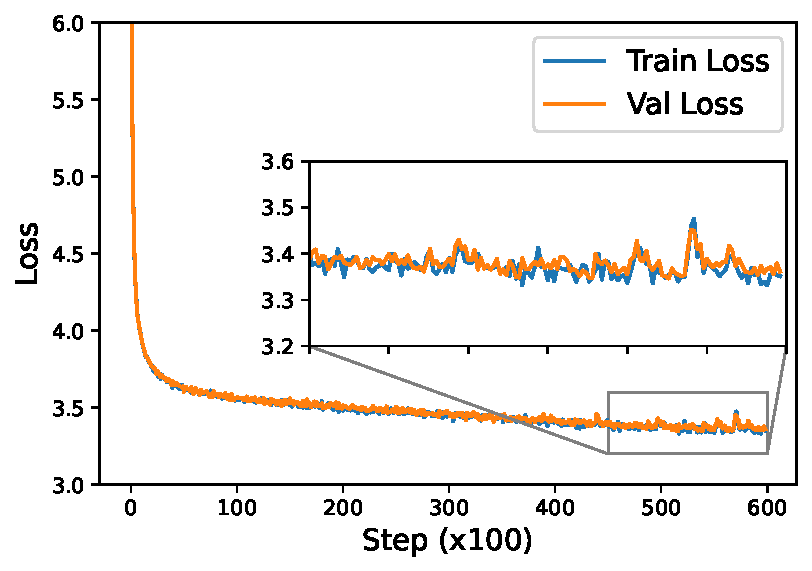
\includegraphics[width=0.5\textwidth]{\toplevelprefix/chapters/chapter7/figs/gpt-loss.pdf}
%     \caption{\bf 在OpenWebText数据集上训练的CRATE-GPT-Base的损失曲线。}
%     \label{fig:crate-text-evals}
% \end{figure}

% \subsection{实验设置与结果} 
% \pw{Yifu} 



\section{扩展白盒Transformer}\label{sec:scalable}

在本节中,我们将讨论三种方法,通过这些方法可以扩展CRATE类型模型的不同部分或提高其效率,同时保持其白盒特性。这些进展融合了概念性和经验性的见解,可以被看作是关于如何利用白盒理解来在实践中改进深度学习模型的案例研究。我们用来评估这些方法的任务将是图像分类和下一词元预测,数据分别是ImageNet和OpenWebText,优化过程将是相同的反向传播,唯一改变的是架构。

\subsection{增加网络宽度:CRATE-\texorpdfstring{\(\alpha\)}{alpha}}\label{sub:crate_alpha_experiments}

CRATE框架强制执行的一个设计决策是网络中非线性的\textit{宽度}。在常规Transformer中,宽度通常设置为特征维度的\(4\)、\(8\)或\(\frac{11}{3}\)倍。然而,CRATE强制要求宽度与特征维度完全相等,即字典\(\vD^{\ell}\)是方阵,这可能导致性能下降。CRATE框架限制我们选择此方案的根本原因如下:
\begin{itemize}
    \item ISTA块在字典学习中只执行\textit{单步}优化。
    \item 通常,任何迭代优化算法的一步都不能有效地优化目标。那么为什么这能行得通呢?
    \item 优化算法通常只有在有良好初始化或\textit{热启动}的情况下才会非常快地收敛。ISTA块有热启动——它将输入特征视为所得稀疏编码的初始化。
    \item 这就强制要求输入特征和稀疏编码具有相同的维度。也就是说,ISTA学习一个完备的稀疏化字典(参见\Cref{ch:classic})。
\end{itemize}
因此,如果我们想使用一个宽字典,就需要ISTA执行\textit{过完备}字典学习。这意味着我们不能有相同的热启动(因为我们的稀疏编码的维度比我们的特征大),并且需要更多的迭代来收敛到一个稀疏编码。因此,从特征\(\vZ_{\theta}^{\ell + 1/2}\)到稀疏编码\(\vZ_{\theta}^{\ell + 1}\)的步骤将不再是
\begin{equation}
    \vZ_{\theta}^{\ell + 1} = \ISTA_{\theta}^{\ell}(\vZ_{\theta}^{\ell + 1/2} \mid \vZ_{\theta}^{\ell + 1/2})
\end{equation}
其中\(\ISTA_{\theta}^{\ell}\)函数(滥用前面章节的记号)定义为
\begin{equation}
    \ISTA_{\theta}^{\ell}(\vZ \mid \vY) := \ReLU(\vZ - \beta (\vD^{\ell})^{\top}(\vD^{\ell}\vZ - \vY) + \beta \lambda \vone_{s}\vone_{n}^{\top})
\end{equation}
而是以下迭代:
\begin{equation}
    \vZ_{\theta}^{\ell + 1} = \vA_{\theta}^{\ell, T}; \qquad \vA_{\theta}^{\ell, t + 1} = \ISTA_{\theta}^{\ell}(\vA_{\theta}^{\ell, t} \mid \vZ_{\theta}^{\ell + 1/2}) \quad \forall 0 \leq t < T; \qquad \vA_{\theta}^{\ell, 0} = \vzero_{s \times n},
\end{equation}
即,在每层的前向传播中,在LASSO目标上运行近端梯度法\(T \geq 1\)步,并从\(\vzero_{s \times n}\)初始化。在这种情况下,字典可以根据需要设置宽度,即\(\vD^{\ell} \in \R^{s \times d}\),其中\(s \geq d\)(在实践中通常取\(s = 4d\))。

然而,这带来了一个经验性问题。使用上述配置,如果\(\vZ^{\ell + 1/2} \in \R^{d \times n}\),那么\(\vZ^{\ell + 1} \in \R^{s \times n}\),其特征维度可以任意大。在实践中,我们希望每层的特征维度保持相同。因此,这为设计网络设置了一个实践上的三难困境,即我们\textit{不能}同时拥有以下\textit{所有}期望的特性:
\begin{enumerate}
    \item 每层的特征维度相同。
    \item 字典是宽的,即过完备的。
    \item 非线性的输出是输入相对于字典的稀疏编码。
\end{enumerate}
在实践中,出于效率原因,放弃(1)不太可行。放弃(2)导致常规的CRATE框架。放弃(3)导致CRATE的一个宽版本,即CRATE-\(\alpha\),它具有以下非线性来从\(\vZ^{\ell + 1/2}\)得到\(\vZ^{\ell + 1}\):
\begin{equation}
    \vZ_{\theta}^{\ell + 1} = \vD^{\ell}\vA_{\theta}^{\ell, T}; \qquad \vA_{\theta}^{\ell, t + 1} = \ISTA_{\theta}^{\ell}(\vA_{\theta}^{\ell, t} \mid \vZ_{\theta}^{\ell + 1/2}); \qquad \vA_{\theta}^{\ell, 0} = \vzero,
\end{equation}
即,取通过近端梯度下降获得的稀疏编码,并乘以字典,以获得输入的去噪版本。因此,CRATE-\(\alpha\)的非线性计算的是输入的去噪版本,该版本适合稀疏编码,而不是实际的稀疏编码本身。这里从\(\vZ_{\theta}^{\ell + 1/2}\)到\(\vZ_{\theta}^{\ell + 1}\)的映射被称为过完备字典学习(ODL)块,并表示为\(\operatorname{ODL}_{\theta}^{\ell}\),即
\begin{equation}
    \vZ_{\theta}^{\ell + 1}(\vX) := \operatorname{ODL}_{\theta}^{\ell}(\vZ_{\theta}^{\ell + 1/2}(\vX)).
\end{equation}

\begin{figure}
    \centering 
    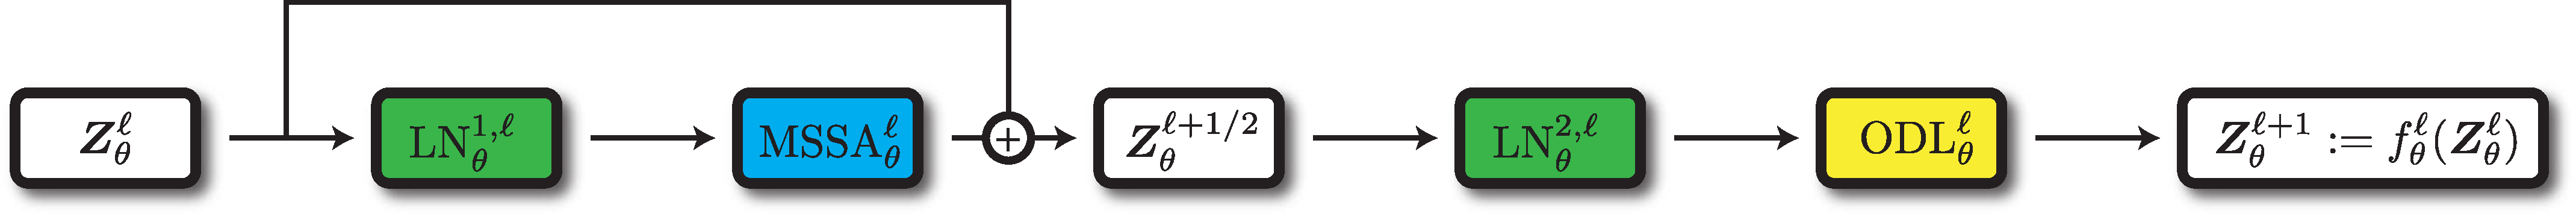
\includegraphics[width=\textwidth]{\toplevelprefix/chapters/chapter7/figs/crate_alpha_backbone.pdf}
    \caption{\small\textbf{CRATE-\(\alpha\)主干网络的一层。}与CRATE的不同之处在于,\(\ISTA_{\theta}^{\ell}\)块被\(\operatorname{ODL}_{\theta}^{\ell}\)块取代,后者使用过完备字典执行多步\(\ISTA\)。}
    \label{fig:crate_alpha_backbone}
\end{figure}

\begin{figure}
    \centering 
    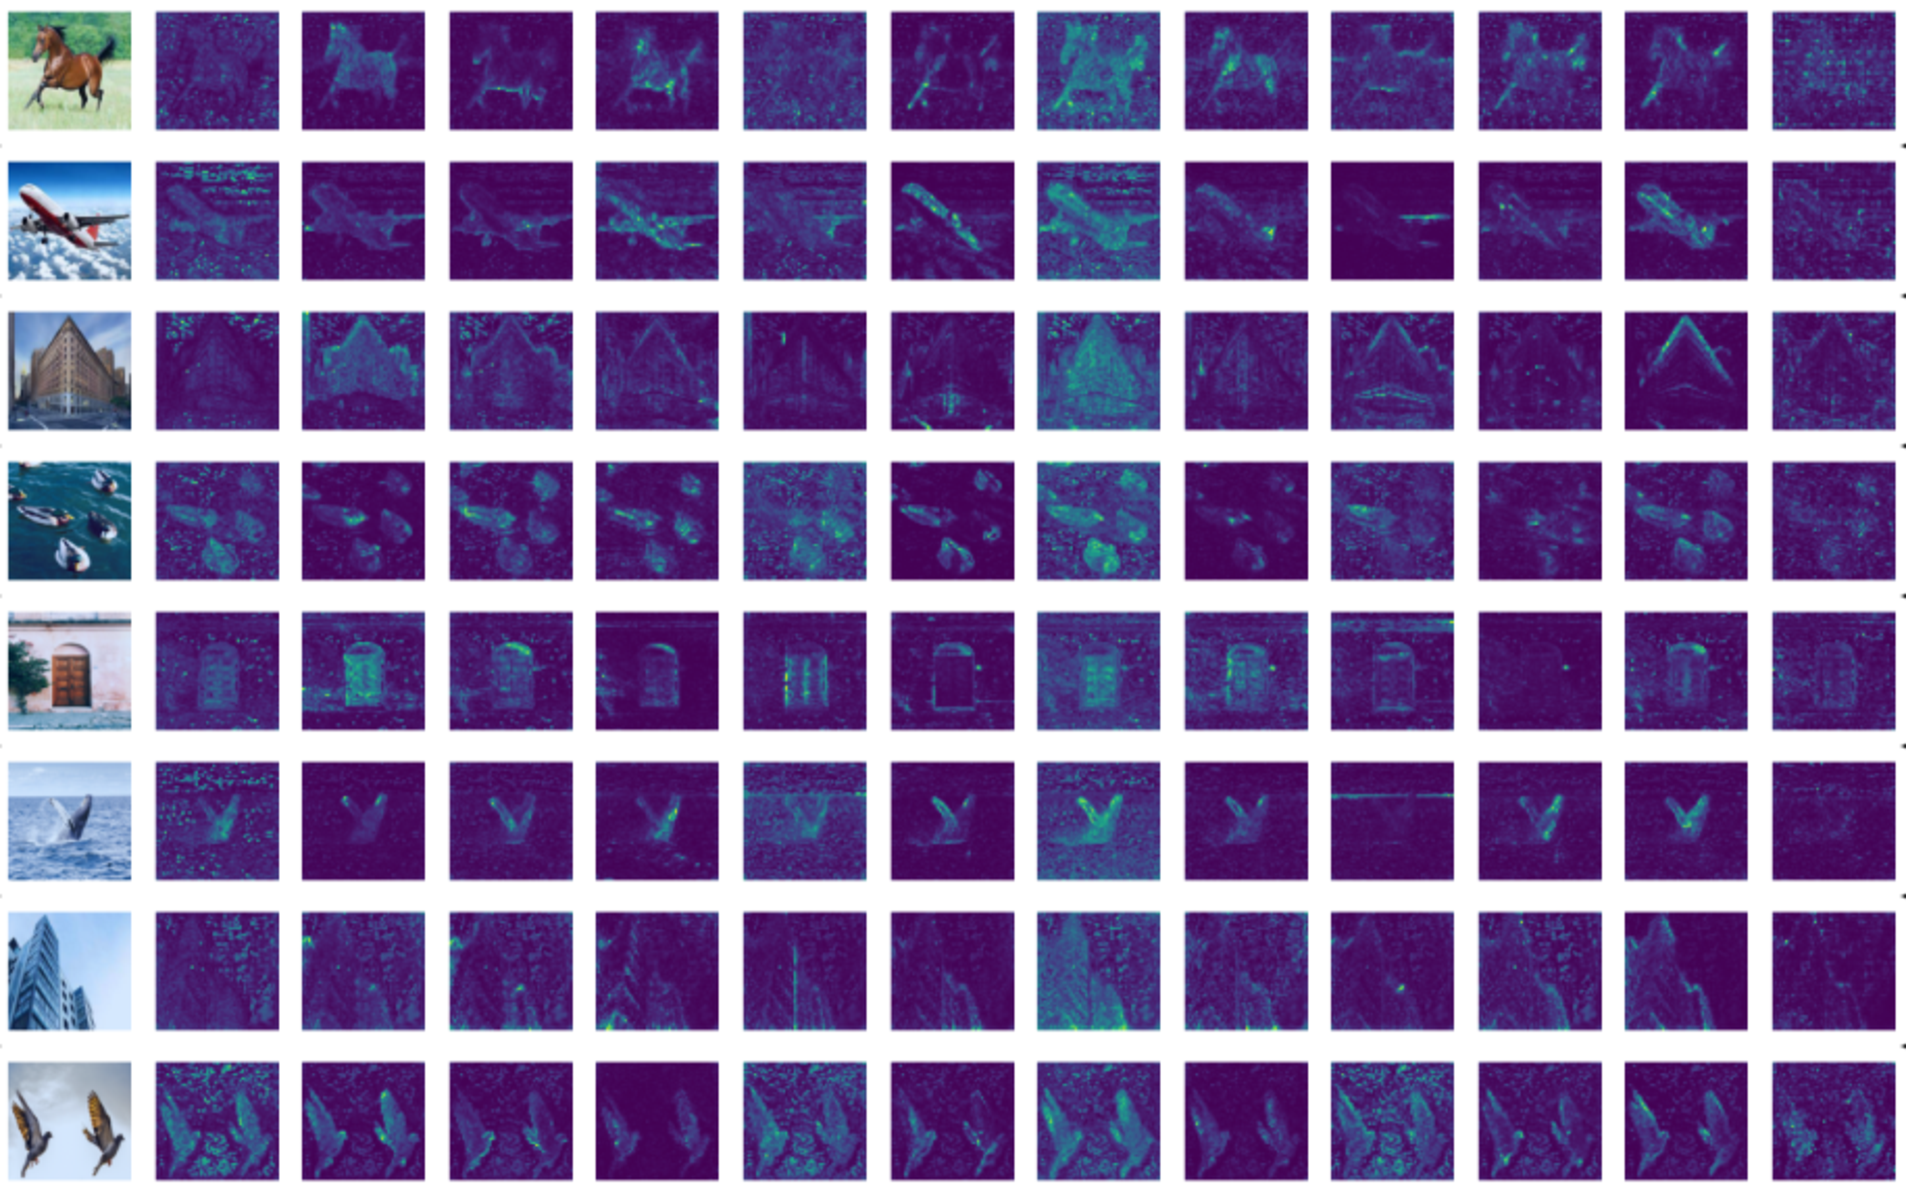
\includegraphics[width=\textwidth]{\toplevelprefix/chapters/chapter7/figs/crate_alpha_semantic_heads.pdf}
    \caption{\small\textbf{来自CRATE-\(\alpha\)的显著图,图像块大小为\(8\)。}每一行是不同的图像,每一列对应最后一层中一个不同的注意力头。我们观察到,显著图与输入图像中的对象有很强的对应关系。}
    \label{fig:crate_alpha_saliency_maps}
\end{figure}

\begin{table}
    \centering
    \begin{tabular}{@{}lcccccccc@{}}
    \toprule
     &  & \multicolumn{3}{c}{检测} &  \multicolumn{3}{c}{分割} \\ 
    模型 & AP$_{50} \uparrow $ & AP$_{75} \uparrow $ & AP $\uparrow$ & AP$_{50} \uparrow$ & AP$_{75} \uparrow $ & AP $\uparrow$ \\ 
    \midrule
    \midrule
    CRATE-\(\alpha\)-B/8 & 3.5 & 1.1 & 1.5 & 2.2 & 1.0 & 1.1 \\
    CRATE-\(\alpha\)-L/8 & \textbf{4.0} & \textbf{1.7} & \textbf{2.0} & \textbf{2.7} & \textbf{1.1} & \textbf{1.4} \\
    \midrule
    \color{gray}CRATE-B/8 & \color{gray}2.9 & \color{gray}1.0 & \color{gray}1.3 & \color{gray}2.2 & \color{gray}0.7 & \color{gray}1.0 \\
    \color{gray}ViT-B/8 & \color{gray}0.8 & \color{gray}0.2 & \color{gray}0.4 & \color{gray}0.7 & \color{gray}0.5 & \color{gray}0.4 \\
    \bottomrule
    \end{tabular}
    \caption{\small \textbf{在COCO val2017~\citep{lin2014microsoft}上通过MaskCut进行的目标检测和细粒度分割}。此处所有模型均使用大小为\(8\)的图像块进行训练,而非\(16\)。与现有的模型如CRATE和ViT相比,CRATE-\(\alpha\)模型家族在性能和可扩展性方面都有显著提升。}
    \label{tab:crate_alpha_detection_segmentation}
\end{table}

\begin{table}
    \centering 
    \begin{tabular}{@{}lcccc@{}}
    \toprule
    模型 & GPT-2-B(ase) & CRATE-B & CRATE-\(\alpha\)-S(mall) & CRATE-\(\alpha\)-B \\ 
    \midrule
    \midrule
    \# 参数 & 124M & 60M & 57M & 120M \\
    OWT 验证损失 & 2.85 & 3.37 & 3.28 & 3.14 \\
    \bottomrule
    \end{tabular}
    \caption{\small\textbf{语言建模中的验证损失。} 此处所有模型都在大部分OpenWebText上进行预训练,验证交叉熵损失是在OpenWebText的一个留出子集上测量的。CRATE-\(\alpha\)相较于CRATE设计有显著改进,尽管与传统Transformer如GPT-2仍存在差距。}
    \label{tab:crate_alpha_lm}
\end{table}

CRATE-\(\alpha\)层如\Cref{fig:crate_alpha_backbone}所示。在实践中,这种对CRATE的修改在更大规模上表现非常好。例如,当我们在ImageNet-21K上预训练CRATE-\(\alpha\)模型时,像分割这样的无监督任务(参见\Cref{fig:crate_alpha_saliency_maps}和\Cref{tab:crate_alpha_detection_segmentation})通常比CRATE有显著的性能提升。在使用因果自注意力的语言模型训练中也存在类似的趋势(参见\Cref{tab:crate_alpha_lm})。总的来说,这是将性能扩展到与黑盒模型(如Transformer)相匹配的一个有前景的途径。\footnote{请注意,本节中的实验结果使用了一个略有不同的模型架构,这带来了非常微小的经验增益。改动是:(1) ODL块上增加了一个残差连接,(2) 修改\(\ISTA\)以使用两个独立的字典,而不是\(\vD^{\ell}\)和\((\vD^{\ell})^{\top}\)。}

%\DP{@YM: note that CRATE-\(\alpha\) paper has no linear probing experiments, only full fine-tuning. Since full fine-tuning doesn't make sense from representation learning perspective, we omit it. Feel free to delete this comment when you are done reading.} That is ok.

\subsection{线性时间复杂度Transformer}\label{sub:tost_experiments}

在实践中,深度学习模型在空间和时间复杂度方面存在瓶颈,这代表了在给定固定资源的情况下它们无法扩展处理的问题规模。其中一个瓶颈,在处理每个样本本身都是高维和丰富的数据(如长文本流或视频)时尤其有意义,那就是处理长序列数据的\textit{时间复杂度}。为了缓解使用Transformer处理数据的时间复杂度问题,我们在\Cref{sub:tost}中提出了一个\textit{词元统计自注意力}算子\(\TSSA_{\theta}^{\ell}\)。我们现在围绕它构建一个\textit{词元统计Transformer},称为ToST,我们可以用它来处理长上下文任务。特别地,我们可以使用以下层(在\Cref{fig:tost_backbone}中描绘)作为CRATE中主干层的直接替代品:
\begin{align}
    \vZ_{\theta}^{\ell + 1/2}(\vX)
    &= \vZ_{\theta}^{\ell}(\vX) + \TSSA_{\theta}^{\ell}(\LN_{\theta}^{1, \ell}(\vZ_{\theta}^{\ell}(\vX))) \\ 
    \vZ_{\theta}^{\ell + 1}(\vX)
    &= \vZ_{\theta}^{\ell + 1/2}(\vX) + \MLP_{\theta}^{\ell}(\LN_{\theta}^{2, \ell}(\vZ_{\theta}^{\ell + 1/2}(\vX)))
\end{align}
其中\(\TSSA\)块的定义如\Cref{sub:tost}中所述。请注意,这与\Cref{sub:contrastive_learning_architecture}中讨论的视觉Transformer架构完全相同,只是\(\TSSA\)取代了传统的多头自注意力块\(\MHSA\)。无论如何,该层前向传播的计算复杂度在所有问题变量——序列长度、特征维度、头数和头维度——上都是线性的。

\begin{figure}
    \centering 
    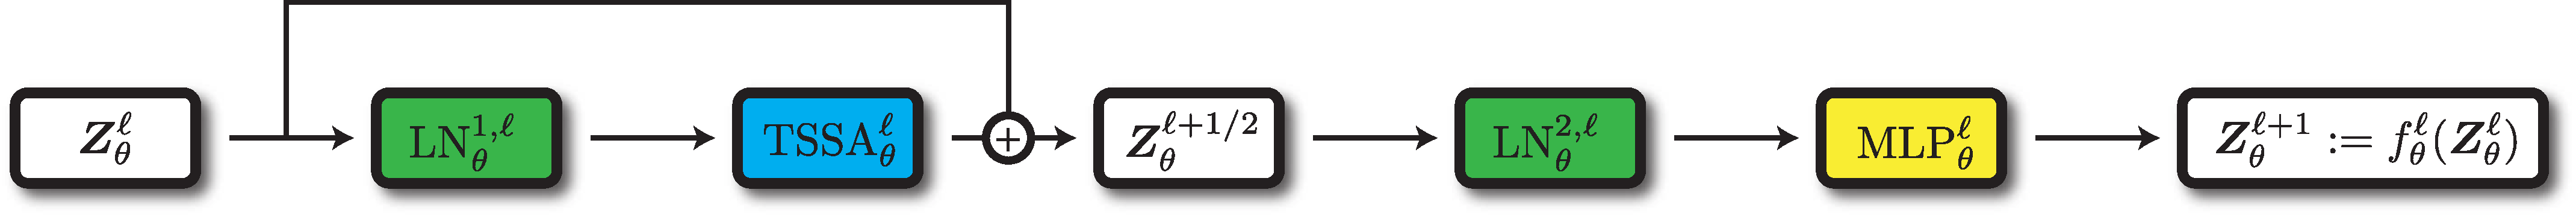
\includegraphics[width=\textwidth]{\toplevelprefix/chapters/chapter7/figs/tost_backbone.pdf}
    \caption{\small\textbf{ToST主干网络的一层}。词元表示依次通过层归一化、词元统计自注意力(TSSA)算子和一个MLP,以形成该层的输出。}
    \label{fig:tost_backbone}
\end{figure}

\begin{table}
    \centering 
    \resizebox{\textwidth}{!}{
    \begin{tabular}{@{}lccc|cc|cc@{}}
    \toprule
    数据集 & ToST-T(iny) & ToST-S(mall) & ToST-M(edium) &  { \color{gray} XCiT-S} &  { \color{gray}XCiT-M} &  {\color{gray}ViT-S} & {\color{gray}ViT-B(ase)}\\ 
    \toprule
     \# 参数 & 5.8M & 22.6M & 68.1M &  { \color{gray}24.9M }& { \color{gray}80.2M } & { \color{gray} 22.1M } & { \color{gray}86.6 M } \\
    \midrule
     ImageNet & 67.3 & 77.9 & 80.3 &  { \color{gray} 80.5} & { \color{gray} 81.5 } & { \color{gray} 79.8} & { \color{gray} 81.8} \\
     ImageNet ReaL & 72.2  & 84.1 & 85.6 &  { \color{gray} 85.6 } & { \color{gray} 85.9} & { \color{gray} 85.6 } & { \color{gray} 86.7 }\\
     \midrule
     CIFAR10 & 95.5 & 96.5 & 97.5 &  { \color{gray} 98.1} & { \color{gray} 98.3} & { \color{gray} 98.6} & { \color{gray} 98.8}\\
     CIFAR100 & 78.3 & 82.7 & 84.5 &  { \color{gray} 86.1} & { \color{gray} 87.6} & { \color{gray} 88.8} & { \color{gray} 89.3}\\
     Oxford Flowers-102 & 88.6 & 92.8 & 94.2 &  { \color{gray} 93.9} & { \color{gray} 94.0} & { \color{gray} 94.0}& { \color{gray} 95.7}\\
     Oxford-IIIT-Pets & 85.6 & 91.1 & 92.8 &  { \color{gray} 92.9} & { \color{gray} 94.0} & { \color{gray} 92.8} & { \color{gray} 94.1} \\
     \bottomrule
    \end{tabular}%
    }
    \caption{\small \textbf{ToST的线性探查分类准确率},在主干网络于ImageNet-1K上进行分类预训练后,在不同数据集和不同模型尺寸下的表现。我们观察到,与XCiT(一种为高效处理长序列而经验设计的类Transformer架构)和ViT相比,ToST保持了相对相似的性能,同时还享有更快的运行时间和白盒设计的优势。}
    \label{tab:tost_linear_probing}
\end{table}

\begin{table}[!htbp]
    \centering 
    \begin{tabular}{@{}lcccccc@{}}
        \toprule
        模型 & \# 参数 & OWT & Lambada & Wikitext & PTB & 平均 $\downarrow$ \\ \midrule
        GPT-2-Base & 124M & 2.84 & 4.32 & 4.13 & 5.75 & 4.26 \\
        ToST-Base & 110M & 3.20 & 4.98 & 4.77 & 6.39 & 4.84 \\
        ToST-Medium & 304M & 2.88 & 4.45 & 4.30 & 5.64 & 4.32 \\
        ToST-Large & 655M & 2.72 & 4.32 & 3.99 & 5.03 & 4.02 \\ \bottomrule
    \end{tabular}%
    \caption{\small\textbf{语言建模验证损失},在各种自然语言数据集的(留出集)上计算,模型在该数据集上进行预训练后。我们观察到ToST扩展性良好,因此ToST-Large在因果语言建模方面超过了基线GPT-2-Base,同时在长上下文中享有更高的效率。}
    \label{tab:tost_lm}
\end{table}

\begin{table}
    \centering
    
    \begin{tabular}{@{}lccccccc@{}}
            \toprule
            模型        & ListOps  & Text     & Retrieval & Image    & Pathfinder & 平均      \\
            \midrule
            \midrule
            Reformer              & \textbf{37.27} & 56.10             & 53.40              & 38.07             & 68.50               & 50.56             \\
            BigBird               & 36.05             & 64.02             & 59.29              & 40.83             & 74.87                & 54.17             \\
            LinFormer         & 16.13             & \underline{65.90} & 53.09              & 42.34             & \underline{75.30}               & 50.46             \\
            Performer             & 18.01             & 65.40             & 53.82              & 42.77             & \textbf{77.05}                & 51.18             \\
            Transformer           & 37.11             & 65.21             & \underline{79.14}              & \underline{42.94}             & 71.83              & \underline{59.24}            \\
            ToST & \underline{37.25}    & \textbf{66.75}    & \textbf{79.46}     & \textbf{46.62}    &    69.41      &     \textbf{59.90}\\
            
            \bottomrule
        \end{tabular}%
    \caption{\small \textbf{ToST(-B)与为长上下文优化的顶级Transformer变体的长程竞技场(LRA)性能比较。}长程竞技场是一系列基准测试,通过固定数据集和评估机制来测试算法和架构的长序列建模能力。与所有已知的Transformer变体(包括XCiT和常规(ViT)Transformer,参见\Cref{tab:tost_linear_probing})相比,ToST在排行榜上名列前茅。此外,ToST具有最低的时间和空间复杂度推理。(在此表中,特定基准测试的最佳分数用粗体表示,次佳分数用下划线表示。)}
    \label{tab:tost_lra_results}
\end{table}

此外,所提出的架构,名为ToST(“Token Statistics Transformer”的缩写),在视觉任务(即\Cref{tab:tost_linear_probing})和语言任务(即\Cref{tab:tost_lm})上表现良好。这在长序列长度任务中尤其如此(参见\Cref{tab:tost_lra_results}),在这些任务中,它比传统Transformer和所有其他类Transformer架构性能更好且效率高得多。

\subsection{纯注意力Transformer} \label{sub:aot_experiments}

深度学习模型,特别是类Transformer架构,需要消除的另一个瓶颈是内存瓶颈,它来自于MLP中的大规模矩阵乘法,其中内部维度远大于特征维度\(d\)。因此,一个有趣且重要的问题是:我们\textit{真的}需要Transformer内部的MLP吗?没有它性能能达到多好?为了探讨这个问题,我们使用纯注意力Transformer(AoT)架构(参见\Cref{sub:aot}),如\Cref{fig:aot_backbone}所示。也就是说,每一层都简单地是这种形式
\begin{equation}
    \vZ_{\theta}^{\ell + 1}(\vX) = \vZ_{\theta}^{\ell}(\vX) + \MSSA_{\theta}^{\ell}(\LN_{\theta}^{\ell}(\vZ_{\theta}^{\ell}(\vX))).
\end{equation}
在我们的实现中,我们还试验了用多头自注意力(MHSA)代替MSSA。事实证明,这种架构\textit{也}是可行的,尽管为了达到与常规CRATE或Transformer架构相当的性能,网络的深度需要更深。% (i.e., \Cref{tab:aot_lm}).

% 此外,所提出的架构在语言任务上表现良好(即\Cref{tab:tost_lm})。这在长序列长度任务中尤其如此(参见\Cref{tab:tost_lra_results}),在这些任务中,它比传统Transformer和所有其他类Transformer架构性能更好且效率高得多。
% \DP{Frankly, the vision benchmark results here are very poor, and I cannot advertise them. I will just put the language benchmark.}

\begin{figure}
    \centering 
    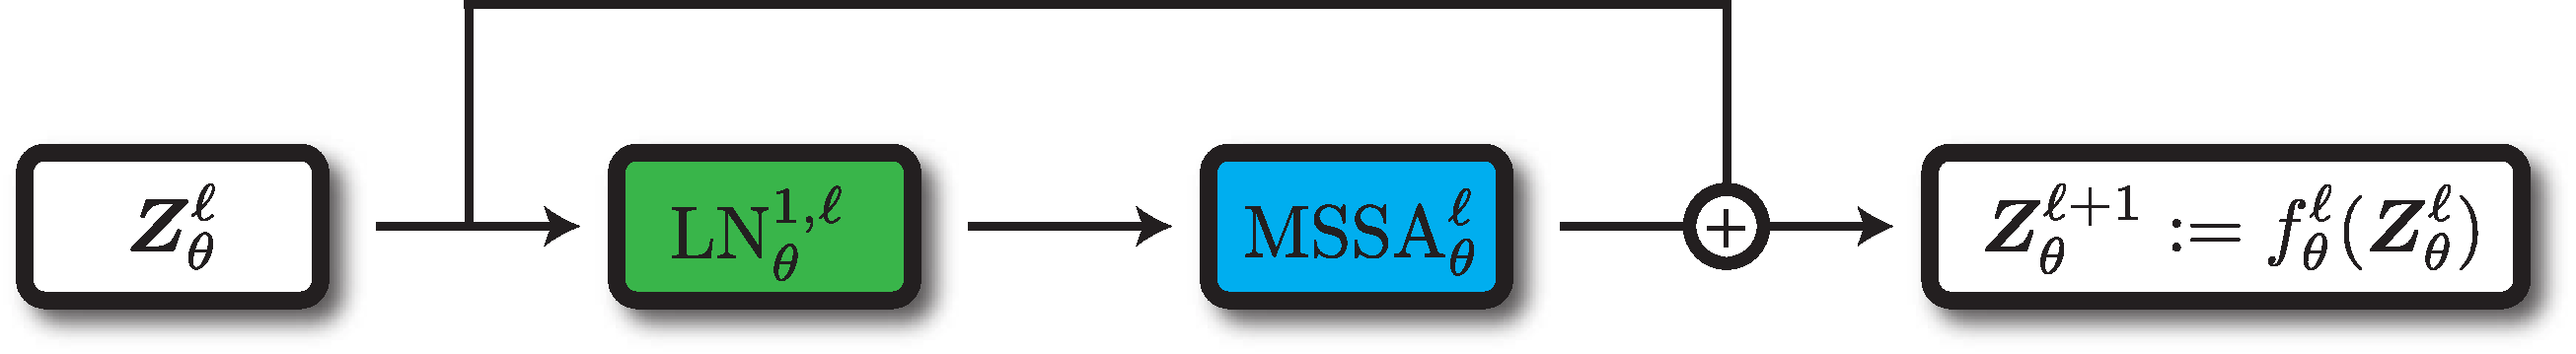
\includegraphics[width=0.7\textwidth]{\toplevelprefix/chapters/chapter7/figs/aot_backbone.pdf}
    \caption{\small\textbf{AoT主干网络的一层。}词元表示仅通过一个层归一化和多头(子空间)自注意力算子来形成该层的输出。请注意,没有像MLP、ISTA或ODL这样的逐词元非线性操作。}
    \label{fig:aot_backbone}
\end{figure}

% \begin{table}
%     \centering 
%     \DP{I think the chart in the AoT Overleaf is wrong (there is Base and Medium model sizes, lol), so I'm omitting it here, for now. TODO @Yifu @Peng}
%     \caption{\small\textbf{AoT在语言建模上的性能},在多个数据集上测量,评估指标为在留出集上测量的验证交叉熵损失。我们可以看到一个有利的扩展趋势:最大版本的AoT比小版本好得多,并且与GPT-2-Base的得分相当。}
%     \label{tab:aot_lm}
% \end{table}

 

\section{图像数据的掩码自编码}\label{sec:image_completion}

我们讨论的第二个应用是\textit{非线性图像补全},也称为\textit{掩码自编码}(Masked Autoencoding, MAE),它是\Cref{ch:classic}中讨论的低秩矩阵补全问题的直接推广。自\cite{he2022masked}在深度学习背景下引入掩码自编码以来,它已成为一种经典且简单的自监督表示学习方法,旨在使\(\vZ_{\theta}\)中的每个图像块特征既包含聚合信息,又包含其邻域信息,从而使图像块特征和聚合特征都成为整个样本的丰富信息来源。

数据集与\Cref{sub:contrastive_learning_data}中讨论的图像数据集保持相同。像往常一样,我们仍然对每个新批次中的每个样本应用数据增强。

\subsection{任务与目标}\label{sub:image_completion_objective}

顾名思义,掩码自编码涉及一个视图\(v_{m}\),该视图在给定输入后,执行随机缩放裁剪(参见\Cref{sub:contrastive_learning_objective})将输入图像转换为大小为\((C, S_{\mask}, S_{\mask})\)的方形图像,然后\textit{掩码}(即设置为零)输入中固定百分比\(p_{\mask} \in [0, 1]\)的像素。出于效率原因\footnote{MAE的原始实现由\cite{he2022masked}提出,它嵌入整个图像,\textit{移除}将被掩码的词元,将得到的词元集送入编码器,在掩码位置添加回学习到的占位符词元并加回相应的位置编码,然后将得到的词元集送入解码器以获得自编码预测。这种方法效率更高,因为编码器需要处理的词元更少,但在概念上与本文讨论的方法相同,并且所得模型在掩码自编码任务和下游评估中的性能非常相似。},掩码是逐图像块进行的,即在嵌入整个图像后,将\(p_{\mask}\)百分比的\textit{图像块}设置为零。MAE的目标是训练一个编码器\(f_{\theta} \colon \cI \to (\R^{d})^{*}\)和一个解码器\(g_{\eta} \colon (\R^{d})^{*} \to \cI\),它们可以从其掩码版本中重建输入,即,记\(\hat{\vX}_{\theta, \eta} := g_{\eta} \circ f_{\theta}\),我们有
\begin{equation}
    \min_{\theta, \eta}\bc{\cL_{\mathrm{MAE}}(\theta, \eta) := \Ex\norm{\hat{\vX}_{\theta, \eta}(\vX_{m}) - \vX}_{F}^{2}}
\end{equation}
这实质上意味着视图\(\vX_{m} := v_{m}(\vX)\)的特征\(\vZ_{\theta}(\vX_{m})\)必须包含关于\textit{被掩码的图像块}以及现有图像块的信息。从\Cref{ch:representation}中基于压缩的白盒模型的角度来看,如果一个白盒自编码器\((f_{\theta}, g_{\eta})\)成功完成了这个任务,这意味着学习到的子空间和字典对数据进行了\textit{冗余}编码,从而可以从数据的其他已编码部分重建数据的缺失部分。这意味着关于每个图像块的信息存储在其他图像块中。因此,我们再次期望表示应包含局部和全局的语义相关信息,因此具有相似局部和全局信息(即在同一子空间上或由同一字典编码)的不同图像块的表示应该是相关的。

\subsection{架构}\label{sub:image_completion_architecture}

\begin{figure}
    \centering 
    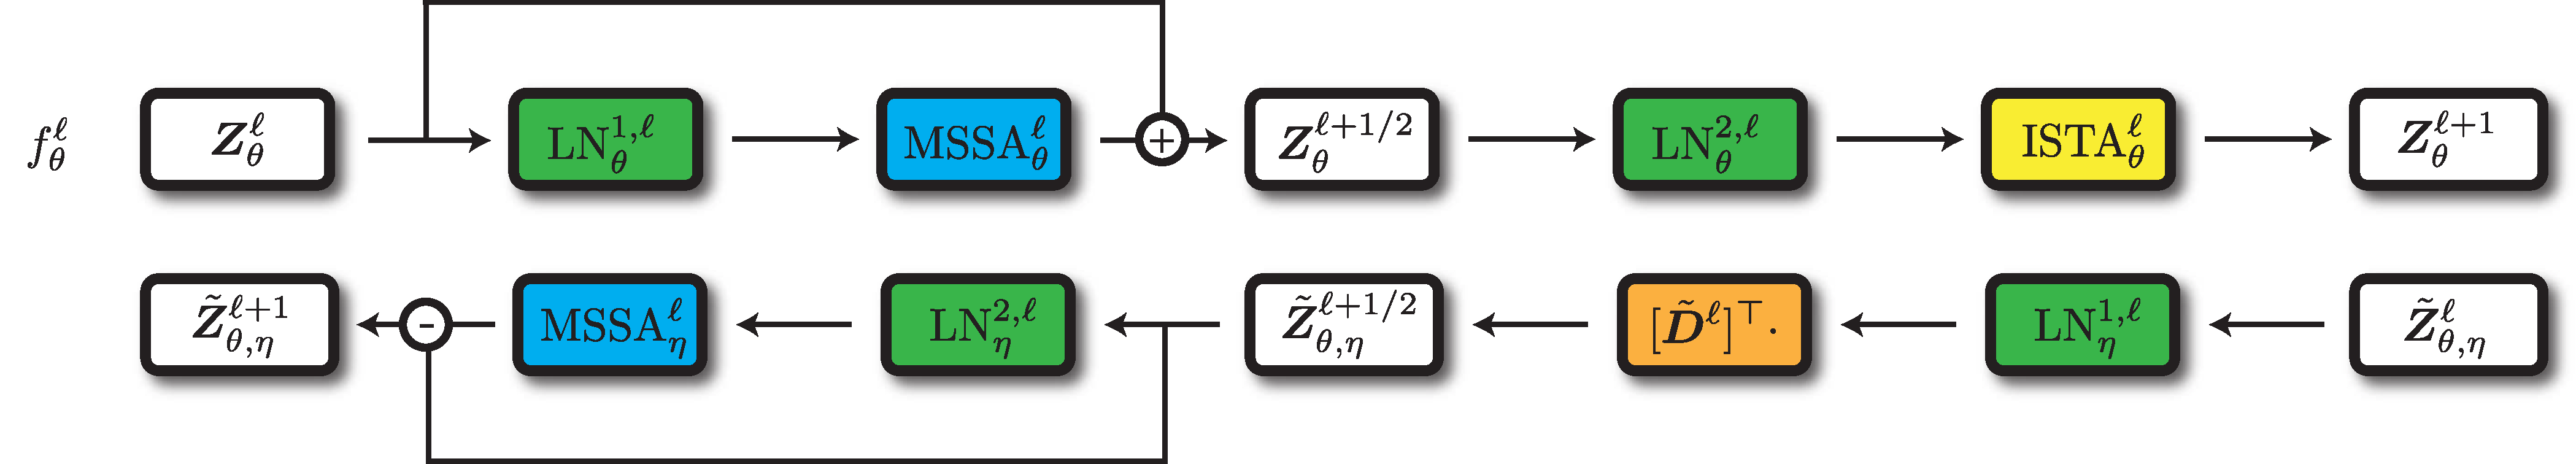
\includegraphics[width=\textwidth]{\toplevelprefix/chapters/chapter7/figs/crate_ae_backbone.pdf}
    \caption{\small\textbf{CRATE自编码器主干网络中编码器和解码器的一层。}编码器和解码器层都将其输入通过多头子空间自注意力和一个字典学习或字典编码步骤。注意,编码器和解码器层是对称设计的;每个解码器层的概念目标是反转一个编码器层,因此这种对称性是经过深思熟虑的设计(例如,参见\Cref{ch:autoencoding})。}
\end{figure}

我们使用一个CRATE编码器和解码器,如\Cref{fig:transformer_backbone}\pw{这个引用正确吗?}所示,当然也可以使用常规的Transformer编码器和解码器。详情如下。

\paragraph{编码器。} 编码器与\Cref{sub:image_classification_architecture}中的CRATE编码器相同,但没有特征提取器\(f_{\theta}^{\ext}\)。然而,嵌入\(f_{\theta}^{\emb}\)和主干网络\(f_{\theta}^{\backbone}\)都是相同的。

\paragraph{解码器主干网络。} 解码器主干网络是\Cref{ch:autoencoding}中描述的CRATE解码器。为完整起见,我们现在对其进行描述。给定一个特征序列\(\vZ_{\theta}(\vX) := f_{\theta}(\vX) \in (\R^{d})^{*}\),我们可以使用解码器主干网络\(g_{\eta}^{\backbone}\)来处理它。函数\(g_{\eta}^{\backbone}\)由\(L\)层\(g_{\eta}^{\ell}\)组成,即
\begin{equation}
    g_{\eta}^{\backbone} = g_{\eta}^{L} \circ \cdots \circ g_{\eta}^{1}.
\end{equation}
层\(g_{\eta}^{\ell}\)的实现如下。首先,定义\(\tilde{\vZ}_{\theta, \eta}^{1}(\vX) := \vZ_{\theta}(\vX)\)。然后,我们得到
\begin{align}
    \tilde{\vZ}_{\theta, \eta}^{\ell + 1/2}(\vX) 
    &= [\tilde{\vD}^{\ell}]^{\top}\LN_{\eta}^{1, \ell}(\tilde{\vZ}_{\theta, \eta}^{\ell}(\vX)) \\ 
    \tilde{\vZ}_{\theta, \eta}^{\ell + 1}(\vX)
    &= \tilde{\vZ}_{\theta, \eta}^{\ell + 1/2}(\vX) - \MSSA_{\eta}^{\ell}(\LN_{\eta}^{2, \ell}(\tilde{\vZ}_{\theta, \eta}^{\ell + 1/2}))
\end{align}
并且\(g_{\eta}^{\ell}\)的定义使得\(g_{\eta}^{\ell}(\tilde{\vZ}_{\theta, \eta}^{\ell}) := \tilde{\vZ}_{\theta, \eta}^{\ell + 1}(\vX)\)。这里的相关概念是,\(g_{\eta}^{\ell}\)应该学习一个\(f_{\theta}^{L + 1 - \ell}\)的近似逆,分别作为前向和反向时间扩散过程的离散化。特别地,\(\tilde{\vD}^{\ell}\)应该近似于\(\vD^{L + 1 - \ell}\),类似地,\(\MSSA_{\eta}^{\ell}\)的参数应该与\(\MSSA_{\theta}^{L + 1 - \ell}\)的参数相似。输出是\(\tilde{\vZ}_{\theta, \eta} := \tilde{\vZ}_{\theta, \eta}^{L + 1}\)。

\paragraph{反嵌入模块。} 为了将\(\tilde{\vZ}_{\theta, \eta}(\vX)\)转换回对\(\vX\)的估计,我们需要使用反嵌入模块\(g_{\eta}^{\unemb}\)来撤销嵌入模块\(f_{\theta}^{\emb}\)的效果。因此,回顾\eqref{eq:definition_of_embedding_module}中嵌入模块的函数形式,即
\begin{equation}
    f_{\theta}^{\emb}(\vX) := \mat{\vz_{\cls}^{1}, \vW^{\emb}f^{\patch}(\vX) + \vE^{\pos}}
\end{equation}
这意味着我们的逆操作\(g_{\eta}^{\unemb}\)看起来如下:
\begin{equation}
    g_{\eta}^{\unemb}(\tilde{\vZ}) := g_{\eta}^{\unemb}(\mat{\tilde{\vz}^{1}, \dots, \tilde{\vz}^{n}}) = g^{\unpatch}(\vW^{\unemb}([\tilde{\vz}^{2}, \dots, \tilde{\vz}^{n}] - \tilde{\vE}^{\pos})),
\end{equation}
其中\(g^{\unpatch}\)执行与\(f^{\patch}\)所做的展开和扁平化操作相反的操作。\footnote{同样,“逆位置编码”\(\tilde{\vE}^{\pos}\)是为大输入学习的,对于较小的输入可能会被插值。甚至可以直接设置\(\tilde{\vE}^{\pos}\)等于位置编码\(\vE^{\pos}\),并在编码器和解码器中对每个输入使用相同的插值位置编码。}

这个架构是一个白盒自编码器\((f_{\theta}, g_{\eta})\),其中(回顾一下)\(f_{\theta} = f_{\theta}^{\backbone} \circ f_{\theta}^{\emb}\)和\(g_{\eta} = g_{\eta}^{\unemb} \circ g_{\eta}^{\backbone}\)。特别地,我们可以用它来计算一个掩码视图的估计\(\hat{\vX}_{\theta, \eta}(\vX_{m}) = (g_{\eta} \circ f_{\eta})(\vX_{m})\),它应该近似等于\(\vX\)本身。

\subsection{优化}\label{sub:image_completion_optimization}

与\Cref{sub:image_classification_optimization}中一样,我们使用一个简单的优化设置:我们对图像和掩码进行采样,计算这些样本上的损失及其梯度,并使用一个通用的优化算法和上述梯度来更新参数。对于每个时间步\(k\),我们:
\begin{itemize}
    \item 子采样\(B\)个不同的样本\(\{\vX_{b}^{(k)}\}_{b = 1}^{B} \subseteq \cI\)。
    \item 对每个样本\(\vX_{b}^{(k)}\),计算一个不同的随机缩放裁剪和掩码\(v_{b, m}^{(k)}\)并将其应用于\(\vX_{b}^{(k)}\)以得到\(\vX_{b, m}^{(k)} := v_{b, m}^{t}(\X_{b}^{(k)})\)。
    \item 计算估计的自编码\(\hat{\vX}_{\theta, \eta}(\vX_{b, r}^{(k)}) := (g_{\eta} \circ f_{\theta})(\vX_{b, r}^{(k)})\)。
    \item 构建代理随机损失
    \begin{equation}
        \hat{\cL}_{\mathrm{MAE}}^{(k)}(\theta, \eta) := \frac{1}{B}\sum_{b = 1}^{B}\norm{\hat{\vX}_{\theta, \eta}(\vX_{b, r}^{(k)}) - \vX_{b}^{(k)}}_{F}^{2}.
    \end{equation}
    \item 对\((\theta, \eta)\)执行一步优化算法,得到以下迭代:
    \begin{equation}
        (\theta^{(k + 1)}, \eta^{(k + 1)}) := \textsc{OptUpdate}^{(k)}(\theta^{(k)}, \eta^{(k)}; \nabla_{(\theta, \eta)}\hat{\cL}_{\mathrm{MAE}}^{(k)}).
    \end{equation}
\end{itemize}

\subsection{评估} \label{sub:image_completion_optimization_1}

这是我们在本章中讨论的第一个自编码器网络。我们使用与\Cref{sub:contrastive_learning_evals,sub:image_classification_evals}中相同的中心裁剪视图\(v_{\cc}\),将最终图像缩放为边长为\(S_{\cc} = S_{\mask}\)像素的正方形,以匹配训练期间看到的输入图像的形状。

除了评估掩码自编码损失本身,还可以直接评估数据\(\vX\)的视图\(\vX_{\cc} := v_{\cc}(\vX)\)的特征\(\vZ_{\theta}(\vX_{\cc})\)。为了进行注意力图保真度评估,仅获得\(\vZ_{\theta}(\vX_{\cc})\)就足够了,但对于线性探查,我们需要从\(\vZ_{\theta}\)中提取一个摘要或聚合特征。为此,我们可以使用一个(无参数的)特征提取映射,它只返回与类别词元对应的特征,即
\begin{equation}
    f_{\theta}^{\ext}(\vZ) := f_{\theta}^{\ext}([\vz^{1}, \dots, \vz^{n}]) = \vz^{1},
\end{equation}
例如,如\Cref{sub:image_classification_objective,sub:image_classification_architecture}中所示。这样,我们就有一种方法来获得聚合特征\(\vz_{\theta}(\vX_{\cc}) := (f_{\theta}^{\ext} \circ f_{\theta})(\vX_{\cc})\),此时我们就可以进行线性探查、分割评估等。

\subsection{实验}\label{sub:image_completion_experiments}

由于CRATE-MAE直接基于ViT-MAE,我们将\citep{he2022masked}给出的ViT-MAE的最优设置与应用于CRATE-MAE的相同设置进行比较,以实现公平对比。

\paragraph{模型架构。} 在训练期间,掩码裁剪\(v_{m}\)将整个图像缩放,使其较短的边长为\(256\)(即\(S_{\rsz} = 256\)),然后进行大小为\(224 \times 224\)的随机裁剪(即\(S_{\mathrm{mask}} = 224\)),并掩码掉\(p_{\mathrm{mask}} = \frac{3}{4}\)的图像块。我们采用的图像块大小为\(16\)(即\(P_{H} = P_{W} = 16\))。我们使用ViT-MAE架构的small和base变体作为编码器和解码器的嵌入和主干,分别用MSSA、ISTA和线性层替换MHSA和MLP组件。在MSSA的情况下,我们使用相同的头数和头维度。然而,原始的ViT-MAE使用一个几乎占用了所有总层数的编码器和一个只使用少数几层的解码器;我们按照\Cref{ch:autoencoding}中的概念和理论框架的建议,将总层数(从ViT-MAE到CRATE-MAE保持不变)的一半分配给我们的编码器和解码器。对于CRATE-MAE,我们设置\((\beta, \lambda) = (1, 0.1)\)。

\paragraph{数据集与优化。} 对于预训练,我们使用ImageNet-1K数据集。我们使用AdamW优化器来预训练我们的ViT-MAE复现模型以及CRATE-MAE。我们设置基础学习率为\(3 \times 10^{-5}\),权重衰减为\(0.1\),批处理大小为\(B = 4096\)。我们的学习率调度方案在前\(40\)个周期内将学习率线性增加至基础学习率,然后在接下来的\(760\)个周期内使用余弦调度将其降至\(0\)(所有模型均训练\(800\)个周期)。在预训练阶段,我们对图像数据应用常规的数据增强方案(翻转、高斯模糊、日晒效果等)。

对于线性探查,我们使用多个评估数据集,如CIFAR10、CIFAR100、Oxford-Flowers和Oxford-IIT-Pets。对于线性探查,我们预先计算目标数据集中所有样本的特征,并应用一个快速的线性回归求解器,例如来自Scikit-Learn等标准包的求解器。

\paragraph{实验结果。} \Cref{tab:crate_mae_linear_probing}表明,CRATE-MAE模型在相似参数数量下,与流行的ViT-MAE架构相比,大致达到了同等的性能,并且特征学习性能(通过下游分类任务的性能衡量)随着规模的增加而提高。同时,\Cref{fig:crate_mae_semantic_heads}表明,编码器的显著图(因此也是编码器学习到的细粒度特征)确实分离并突显了输入图像的关键部分。


\begin{table}
    \centering 
    \begin{tabular}{@{}lcc|cc@{}}
        \toprule 
        \textbf{模型} & CRATE-MAE-S(mall) & CRATE-MAE-B(ase) & {\color{gray} ViT-MAE-S} & {\color{gray} ViT-MAE-B} \\
        \midrule
        \midrule
        \# 参数 & 25.4M & 44.6M & 47.6M & {\color{gray}143.8M} \\
        \midrule
        CIFAR10 & 79.4 & 80.9 & {\color{gray} 79.9} & {\color{gray} 87.9} \\
        CIFAR100 & 56.6 & 60.1 & {\color{gray} 62.3} & {\color{gray} 68.0} \\
        Oxford Flowers-102 & 57.7 & 61.8 & {\color{gray} 66.8} & {\color{gray} 66.4} \\
        Oxford-IIIT-Pets & 40.6 & 46.2 & {\color{gray} 51.8} & {\color{gray} 80.1} \\
        \bottomrule
    \end{tabular}
    \caption{\small\textbf{CRATE-MAE和ViT-MAE的线性探查分类准确率},在主干网络于ImageNet-1K上进行掩码自编码预训练后,在不同数据集和不同模型尺寸下的表现。在相同的参数数量下,CRATE-MAE取得了大致相似的性能,同时享有更简单、更有原则的架构设计。}
    \label{tab:crate_mae_linear_probing}
\end{table}

\begin{figure}
    \centering 
    \includegraphics[width=\textwidth]{\toplevelprefix/chapters/chapter7/figs/crate_mae_semantic_heads.pdf}
    \caption{\small\textbf{CRATE-MAE的显著图。}每对图像由原始图像(左)和选定的显著图(右)组成,后者对应于最后一层的一个注意力头。与CRATE模型通常的情况一样,但与一般的类Transformer模型不同,显著图对应于输入图像中的对象。}
    \label{fig:crate_mae_semantic_heads}
\end{figure}

% \section{文本数据的掩码补全}\label{sec:text_completion}

% \section{图像的闭环转录}\label{sec:ctrl}


% \section{大规模模型训练技巧}\label{sec:training_tips}

\section{总结与注释}

本章的所有工作都源于\citet{vaswani2017attention}引入的Transformer架构。Transformer架构在\Cref{sec:contrastive_learning}中有正式描述。近年来,受Transformer架构的普及和性能的推动,一个主要的经验性创新是将给定的学习问题表述为序列到序列问题,并应用Transformer架构。这使得Transformer架构在(几乎)所有深度学习应用中无处不在。因此,对Transformer的直接改进可以传播为许多问题的解决方案,并产生相当大的影响;同样,我们可以将我们对类Transformer架构的白盒理解应用于许多现代问题。本章所涵盖的材料仅仅是已完成工作的一个子集;其他工作包括文本数据的掩码补全(即BERT)\citep{devlin2019bert,yu2024white}、语言和视觉模型的(机理)可解释性\citep{bai2024improving}以及纠错码\citep{zheng2025white}。还有更多的工作有待完成。

此外,还有更多关于神经网络扩展实践的理论,这在实践中具有巨大的可行性,我们至少在这里提及一下。这一系列工作由“张量程序”系列工作\citep{yang2022tensor}推广开来。其基本方案是,我们希望Transformer中的初始梯度更新大小恒定,通过仔细研究反向传播方程(\Cref{app:optimization}),我们可以确定实现这一目标所需的初始化尺度和学习率(逐层选择)。在实践中,这样的方案极大地提高了大规模训练的稳定性和收敛性;它们还提供了一种仅使用小规模训练来找到大规模训练的“最优”\footnote{“最优”一词用引号,因为这方面的工作仅仅使用关于初始化时的权重大小、特征大小和梯度大小的一些期望特性来确定“最优性”,而不是,比如说,收敛时的测试损失。}超参数的方法。这项工作的后续研究试图适应特征几何\citep{bernstein2024oldoptimizernewnorm},这可以从本书关于表示学习的工作中获得启发。其他后续工作将这种逐权重的信息整合到优化器本身中,以自动获得这些扩展优势,从而得到了像Muon \citep{jordan6muon}这样的优化器,最近这些优化器已被用于非常稳定地训练万亿参数模型\citep{moonshot2025kimi}。总的来说,这两种深度学习理论方法是正交或互补的。


\section{练习与扩展}

\begin{exercise}
    阅读DINO论文\cite{caron2021emerging}。
\end{exercise}

\begin{exercise}
    DINO v2 \cite{oquab2023dinov2}使用了DINO v1的所有内容,但在数据增强阶段,还随机掩码了每个视图内的图像块。这种增强应该强制具有相似局部信息的图像的特征是相似的。请构建一个在编码器中促进这一点的优化问题,并实现它。
\end{exercise}


\begin{exercise}
    本练习考虑了最小化涉及期望的损失的随机优化算法的实现。
    \begin{enumerate}[(a)]
        \item 提出一个替代\eqref{eq:simdino_loss_teacherstudent_empirical}中涉及\(R_{\eps}\)的项的方法,以近似\eqref{eq:simdino_loss_teacherstudent}中的协方差正则化项。评估计算您提出的项及其梯度所需的时间复杂度。分析应包括在单个计算节点与多个节点上计算的情况。
        \item  评估计算\eqref{eq:simdino_loss_teacherstudent_empirical}中现有项及其梯度所需的时间复杂度。
    \end{enumerate}
\end{exercise}

\begin{exercise}
    证明\eqref{eq:linear_probing}和\eqref{eq:linear_probing_empirical}是凸优化问题。
\end{exercise}

\begin{exercise}
    \phantom{}
    \begin{enumerate}[(a)]
        \item 实现CRATE和CRATE-\(\alpha\)模型。
        \item 在CIFAR-10数据集上比较它们的性能和效率。
        \item 从两个方面比较它们的可解释性:
        \begin{itemize}
            \item 表示\(\vZ\)的稀疏性\(\norm{\vZ}_{0}\)。
            \item 注意力图\(\va_{\theta}^{k, \ell}\)。
        \end{itemize}
    \end{enumerate}
\end{exercise}

\end{document}
